% ==============================================================================
% Fichier     : Cours.tex
% Titre       : Analyse de Risque, Audit et Gestion de Crise
% Auteur      : MINKA MI NGUIDJOÏ Thierry Emmanuel
% Institution : Université de Yaoundé I - Ecole Nationale Supérieure Polytechnique - Département de Génie Informatique — LIMSI
% Année       : 2025-2026
% Description : Fichier principal. Orchestre 29 chapitres répartis en 4 modules.
% Compilateur : pdflatex + biber
%   → pdflatex Cours && biber Cours && pdflatex Cours && pdflatex Cours
% ==============================================================================

\documentclass[12pt, a4paper, twoside, openright]{book}

\usepackage{Style_cours}
\addbibresource{bibliographie.bib}

\hypersetup{
    pdftitle  = {Analyse de Risque, Audit et Gestion de Crise},
    pdfauthor = {MINKA MI NGUIDJOÏ Thierry Emmanuel},
    pdfsubject= {Cours universitaire — Gouvernance SI, EBIOS RM, ISO 27001, PCA, Cellule de Crise},
    pdfkeywords={Analyse de Risque, Audit SI, Gestion de Crise, EBIOS RM, ISO 27001,
                 ISO 19011, ISO 22301, RSSI, RETEX, PCA, Université de Yaoundé I}
}

% ==============================================================================
\begin{document}
% ==============================================================================

% ---------------------------------------------------------------------------
% 1. PAGE DE TITRE
% ---------------------------------------------------------------------------
\begin{titlepage}
\thispagestyle{empty}
\pagecolor{CouleurPrimaire}

\begin{tikzpicture}[remember picture, overlay]
    \fill[CouleurAccent]
        (current page.south west) rectangle
        ([yshift=2.2cm] current page.south east);
    \fill[CouleurAccent]
        ([yshift=-1.5cm] current page.north west) rectangle
        ([yshift=-1.8cm] current page.north east);
    % Déco : cercles concentiques (symbolise le cycle PDCA)
    \foreach \r in {4,5.5,7} {
        \draw[white, opacity=0.04, line width=8pt]
            ([xshift=11cm, yshift=-6cm] current page.north west) circle (\r cm);
    }
\end{tikzpicture}

\vspace*{1.5cm}

\begin{center}
    {\color{white!80!gray}\small\scshape
        Université de Yaoundé~I~·~Ecole Nationale Supérieure Polytechnique~·~Département de Génie Informatique}\\[0.4ex]
    {\color{CouleurAccent}\rule{0.55\linewidth}{0.8pt}}
\end{center}

\vspace{1.5cm}

\begin{center}
    {\color{white!60!gray}\footnotesize\scshape cours universitaire}\\[1ex]
    {\color{white}\fontsize{30}{38}\selectfont\bfseries
        Analyse de Risque,}\\[0.3ex]
    {\color{white}\fontsize{30}{38}\selectfont\bfseries
        Audit}\\[0.3ex]
    {\color{CouleurAccent}\fontsize{28}{36}\selectfont\bfseries
        et Gestion de Crise}\\[1.5ex]
    {\color{white!85!gray}\Large\itshape
        Gouvernance, Conformité, Résilience et RETEX}
\end{center}

\vspace{1.5cm}

\begin{center}
    {\color{white!70!gray}\small
        \ding{229}\quad Cas fil rouge : Entreprise LiZbiZ (E-commerce \& Logistique)}\\[0.5ex]
    {\color{white!70!gray}\small
        \ding{44}\quad EBIOS RM~·~ISO 27001/27005~·~ISO 19011~·~ISO 22301~·~ISO 27035}\\[0.5ex]
    {\color{white!70!gray}\small
        \ding{228}\quad Cycle PDCA~·~Matrice RACI~·~PCA/PRA~·~Cellule de Crise~·~RETEX}
\end{center}

\vfill

\begin{center}
    {\color{CouleurAccent}\rule{0.7\linewidth}{1.2pt}}\\[1.2ex]
    {\color{white}\large\bfseries MINKA MI NGUIDJOÏ Thierry Emmanuel}\\[0.4ex]
    {\color{white!80!gray}\small
        CISA~·~CISM~·~CGEIT~·~CRISC~·~CDPSE}\\[0.3ex]
    {\color{white!70!gray}\footnotesize\itshape
        Chercheur — LIMSI — ENSP, Université de Yaoundé~I}\\[0.3ex]
    {\color{white!70!gray}\footnotesize\itshape
        Expert Judiciaire~—~Consultant~—~Cadre supérieur, Contrôle Supérieur de l'État}\\[1.2ex]
    {\color{CouleurAccent}\rule{0.7\linewidth}{1.2pt}}
\end{center}

\vspace{0.6cm}
\begin{center}
    {\color{white!60!gray}\small Année académique 2025--2026}
\end{center}

\afterpage{\nopagecolor}
\end{titlepage}

% ---------------------------------------------------------------------------
% 2. VERSO COUVERTURE
% ---------------------------------------------------------------------------
\clearpage
\thispagestyle{empty}
\vspace*{\fill}
\begin{center}
    \begin{minipage}{0.78\textwidth}
        \footnotesize\color{CouleurBordInfo}
        \begin{center}
            {\bfseries\color{CouleurPrimaire}
                Analyse de Risque, Audit et Gestion de Crise}\\[0.4ex]
            {\itshape Gouvernance, Conformité, Résilience et RETEX}
        \end{center}
        \vspace{0.8ex}\hrule\vspace{0.8ex}
        \textbf{Auteur :} MINKA MI NGUIDJOÏ Thierry Emmanuel\\
        \textbf{Institution :} Université de Yaoundé~I — ENSP — LIMSI\\
        \textbf{Année :} 2025--2026\\[0.5ex]
        Ce document est un support de cours universitaire. Toute reproduction partielle
        à des fins commerciales est interdite sans l'accord écrit de l'auteur. Les
        certifications CISA, CISM, CGEIT, CRISC et CDPSE sont des marques déposées de
        l'\textbf{ISACA}. EBIOS RM est une méthode de l'\textbf{ANSSI}.\\[0.8ex]
        \hrule\vspace{0.5ex}
        {\centering\itshape
        «~La sécurité n'est ni technique, ni organisationnelle : elle est les deux à la fois.~»}
    \end{minipage}
\end{center}
\vspace*{\fill}

% ---------------------------------------------------------------------------
% 3. DÉDICACE
% ---------------------------------------------------------------------------
\clearpage\thispagestyle{empty}
\vspace*{3cm}
\begin{flushright}
    \begin{minipage}{0.62\textwidth}
        \itshape\large\color{CouleurPrimaire}
        À tous ceux qui, dans les organisations,\\
        prennent la peine de modéliser les risques avant qu'ils ne surviennent,\\
        et le courage de piloter la crise quand elle frappe.\\[1.5ex]
        \normalsize\normalfont\color{CouleurAccent}
        Et à ceux qui comprennent qu'un bon RETEX\\
        vaut mieux que dix bonnes intentions.
    \end{minipage}
\end{flushright}

% ---------------------------------------------------------------------------
% 4. REMERCIEMENTS
% ---------------------------------------------------------------------------
\clearpage\thispagestyle{empty}
\chapter*{Remerciements}
\addcontentsline{toc}{chapter}{Remerciements}

La conception de ce cours a bénéficié de l'expérience conjointe du chercheur et du praticien. L'auteur exprime sa reconnaissance à \textbf{tous les relecteurs anonymes et non} et qui ont contribué à l'enrichissement de cette version. 
Une mention spéciale pour \textbf{le Professeur Hamadou Bâ} Directeur Général de l'Hôpital Général de Garoua, pour son amitié qui nous a permis de confronter  plusieurs de nos idées ici développées avec la réalité de la structure exigeante dont il a lacharge. De même, le Directeur du Contrôle Budgétaire au ministère des finances, \textbf{Madame Tabenyang Augusta épouse Ndjock Arrey}, a été d'un appui significatif dans la rédactionde ce cours, son professionalisme et sa disponiblité forcent l'admiration.

La matière de ce cours a été nourrie par les missions menées au sein des \textbf{Services du Contrôle Supérieur de l'État}, où l'audit n'est pas une abstraction académique mais une responsabilité institutionnelle quotidienne. De même des prestations comme consultant individuel auprès d'entreprises nationales et internationales, ce qui lui donne une dimension transnationale.

À nos étudiants ...

% ---------------------------------------------------------------------------
% 5. TDM, FIGURES, TABLEAUX, CODES
% ---------------------------------------------------------------------------
\clearpage\tableofcontents
\clearpage\listoffigures\addcontentsline{toc}{chapter}{Liste des figures}
\listoftables\addcontentsline{toc}{chapter}{Liste des tableaux}
\lstlistoflistings\addcontentsline{toc}{chapter}{Liste des codes source}

% ==============================================================================
% CORPS DU COURS
% ==============================================================================
\mainmatter

% --- Introduction Générale ---
% ==============================================================================
% Fichier     : chapitres/0_Introduction.tex
% Titre       : Introduction Générale, Analyse de Risque, Audit et Gestion de Crise
% Auteur      : MINKA MI NGUIDJOÏ Thierry Emmanuel
% ==============================================================================

\chapter*{Introduction Générale}
\addcontentsline{toc}{chapter}{Introduction Générale}
\markboth{Introduction Générale}{Introduction Générale}

\begin{flushright}
    \itshape
    <<~Ce qui ne vous tue pas vous rend plus fort\\
    à condition d'en avoir tiré les leçons.~>>\\[0.5ex]
    \small-- Adaptation de Nietzsche, \textit{Crépuscule des idoles}
\end{flushright}

\vspace{1.5ex}

% ==============================================================================
\section*{Contexte et Pertinence}
% ==============================================================================

La cybersécurité contemporaine ne se réduit plus à une question de pare-feux ou de mises à jour. Elle est devenue un enjeu de gouvernance, un défi managérial et une obligation réglementaire qui engage la responsabilité des dirigeants au même titre qu'une décision financière. L'entrée en vigueur du RGPD, la montée en puissance des attaques par rançongiciel et la multiplication des incidents affectant des organisations de toutes tailles ont définitivement ancré la sécurité des systèmes d'information dans l'agenda des comités exécutifs.

Ce cours aborde la sécurité de l'information sous un angle \textbf{stratégique et opérationnel}, articulé autour de trois piliers indissociables : \termecle{anticiper} (analyse de risque), \termecle{vérifier} (audit) et \termecle{réagir} (gestion des incidents et des crises). Ces trois dimensions correspondent précisément au cycle vertueux d'amélioration continue \sigle{PDCA}, Planifier, Réaliser, Vérifier, Améliorer, qui constitue le fil conducteur de l'ensemble du programme.

% ==============================================================================
\section*{Fil Conducteur : L'Entreprise LiZbiZ}
% ==============================================================================

La théorie, aussi rigoureuse soit-elle, n'acquiert de sens qu'à l'épreuve du réel. C'est pourquoi l'intégralité de ce cours est articulée autour d'un \textbf{cas d'entreprise unique et progressif} : l'entreprise \textbf{LiZbiZ}, spécialiste du e-commerce et de la logistique automatisée.

\begin{boxlizbiz}
Tout au long des quatre modules, vous endosserez le rôle de \textbf{consultants mandatés par la DSI} de LiZbiZ. Vous ne serez pas spectateurs : vous analyserez leurs risques réels, réaliserez leur pré-audit ISO 27001, répondrez à leur incident de sécurité et piloterez leur cellule de crise lors d'un exercice de simulation. L'entreprise LiZbiZ constitue votre terrain d'expérimentation, avec ses vulnérabilités, ses contradictions organisationnelles et ses contraintes réglementaires authentiques.
\end{boxlizbiz}

% ==============================================================================
\section*{Objectifs Généraux du Cours}
% ==============================================================================

\begin{boxobjectifs}
À l'issue de ce cours, l'étudiant sera capable de :
\begin{enumerate}
    \item \textbf{Maîtriser les fondements de la gouvernance} du SI (RACI, RSSI, COMEX, alignement stratégique).
    \item \textbf{Conduire une analyse de risque complète} selon les méthodes reconnues : EBIOS RM (ANSSI), ISO 27005, NIST SP 800-30.
    \item \textbf{Planifier et réaliser un audit de sécurité} conforme à l'ISO 19011, avec rapport de non-conformités et plan d'actions correctives.
    \item \textbf{Gérer un incident de sécurité} selon le cycle ISO 27035 : détection, confinement, investigation, éradication, RETEX.
    \item \textbf{Mettre en œuvre un Plan de Continuité d'Activité (PCA)} avec analyse d'impact (BIA), définition du RTO et du RPO, et exercice de restauration.
    \item \textbf{Piloter une cellule de crise} : organisation, communication sous pression, règles des 3T, gestion du porte-parole.
    \item \textbf{Produire un Retour d'Expérience (RETEX)} structuré, incluant l'analyse des causes racines (méthode des 5 Pourquoi, diagramme d'Ishikawa) et un plan d'amélioration hiérarchisé.
    \item \textbf{Communiquer efficacement} avec les décideurs non-techniques (COMEX, PDG) sur des enjeux de cybersécurité.
\end{enumerate}
\end{boxobjectifs}

% ==============================================================================
\section*{Architecture du Cours}
% ==============================================================================

Le cours est structuré en \textbf{quatre modules progressifs}, chacun correspondant à une étape du cycle de vie de la sécurité, du plus stratégique au plus opérationnel.

\medskip
\noindent\textbf{Partie I, Gouvernance et Analyse de Risque}

Elle établit les fondements : gouvernance du SI, matrice RACI, vocabulaire du risque (actif, menace, vulnérabilité, criticité), méthodes EBIOS RM et NIST SP 800-30, application pratique sur LiZbiZ, traitement du risque et Plan d'Action Sécurité.

\medskip
\noindent\textbf{Partie II, Audit et Management de la Qualité}

Elle couvre l'intégralité du processus d'audit selon l'ISO 19011 : déclenchement, préparation, réalisation terrain (entretiens, tests techniques), rapport de non-conformités, plan d'actions correctives, référentiels ISO 27001/9001/COBIT.

\medskip
\noindent\textbf{Partie III, Gestion des Incidents et Continuité}

Elle traite du cycle de vie de l'incident de sécurité (ISO 27035), de l'investigation numérique (forensics légal, chaîne de custode), de la planification de la continuité (BIA, RTO/RPO, sites de secours) et de la mise en œuvre pratique du PCA avec simulation Ransomware.

\medskip
\noindent\textbf{Partie IV, Gestion de Crise et RETEX}

Elle aborde la dimension stratégique et humaine : différence incident/crise, organisation de la cellule de crise, communication sous pression (règle des 3T, \textit{holding statement}), simulation Tabletop et retour d'expérience structuré.

% ==============================================================================
\section*{Posture Pédagogique}
% ==============================================================================

\begin{boxinfo}
\textbf{Prérequis recommandés :}
\begin{itemize}
    \item Notions de base en réseaux informatiques (TCP/IP, protocoles, firewalls).
    \item Connaissance des systèmes d'exploitation Windows et Linux.
    \item Cours d'Audit des SI et/ou Hacking Éthique appréciés en préalable.
    \item Sensibilité au droit numérique (RGPD, responsabilité civile et pénale).
\end{itemize}
\end{boxinfo}

\vspace{2ex}
\begin{center}
    {\color{CouleurAccent}\rule{0.6\linewidth}{1pt}}\\[0.8ex]
    {\small\itshape\color{CouleurPrimaire}
        Ce cours est né de la conviction que la sécurité de l'information\\
        n'est ni une affaire de techniciens seuls, ni une affaire de managers seuls\\
        mais une responsabilité partagée qui exige de maîtriser les deux langages.}\\[0.5ex]
    {\small\bfseries\color{CouleurPrimaire}\auteurcours}
\end{center}


% --- Chapitre 1 & 2 : Introduction et LiZbiZ (avant les parties) ---
\chapter{Introduction Générale}
\label{chap:intro}

\section{Contexte et Enjeux}

La cybersécurité moderne ne se limite plus à la technique. Elle est devenue un enjeu stratégique majeur pour la gouvernance des entreprises.

Pour les futurs ingénieurs et managers, trois compétences sont aujourd'hui indispensables :
\begin{enumerate}
    \item \textbf{Anticiper} : Identifier et évaluer les risques avant l'incident.
    \item \textbf{Vérifier} : Auditer les procédures et la conformité technique.
    \item \textbf{Réagir} : Gérer la crise et assurer la continuité de l'activité.
\end{enumerate}

Ce cours vous permettra de maîtriser le cycle de vie complet de la sécurité de l'information.

\section{Objectifs Pédagogiques}

À l'issue de ce cours, vous serez capable de :
\begin{itemize}
    \item Réaliser une analyse de risque complète (méthode EBIOS RM).
    \item Conduire un audit de sécurité (ISO 19011) et rédiger un rapport.
    \item Mettre en œuvre un plan de continuité d'activité (PCA).
    \item Piloter une cellule de crise et communiquer sous pression.
\end{itemize}

\section{Paysage Normatif}

Le cours s'appuie sur les standards internationaux reconnus. Ils constituent le langage commun des experts.

\begin{center}
\begin{tabular}{ll}
    \toprule
    \textbf{Domaine} & \textbf{Normes de référence} \\
    \midrule
    Gestion du Risque & \iso{31000}, \iso{27005}, EBIOS RM \\
    Management Sécurité & \iso{27001}, \iso{9001} \\
    Audit & \iso{19011}, COBIT \\
    Continuité & \iso{22301}, \iso{27035} \\
    \bottomrule
\end{tabular}
\end{center}

\section{Approche Pédagogique : Le Cycle PDCA}

Nous suivrons le cycle d'amélioration continue (PDCA - Plan Do Check Act) comme fil conducteur :

\begin{itemize}
    \item \textbf{Plan (Planifier) :} Analyse de risque et définition de la politique.
    \item \textbf{Do (Réaliser) :} Mise en œuvre des mesures techniques.
    \item \textbf{Check (Vérifier) :} Audit et mesure de l'efficacité.
    \item \textbf{Act (Améliorer) :} Gestion des incidents, crise et RETEX.
\end{itemize}

\section{Le Cas Pratique : Immersion}

La théorie ne suffit pas. Ce cours est articulé autour d'un cas d'entreprise unique et réaliste : \textbf{LiZbiZ}.

\begin{boxlizbiz}
Vous ne serez pas de simples spectateurs. Vous agirez en tant que consultants ou membres de la DSI de l'entreprise \textbf{LiZbiZ}. 
    
Un laboratoire virtuel (GNS3) simulant leur Système d'Information vous sera fourni. Chaque module du cours s'appuiera sur ce cas concret pour appliquer les concepts théoriques.
\end{boxlizbiz}

Le chapitre suivant présente en détail l'entreprise LiZbiZ et son architecture technique.


% ==============================================================================
% Fichier : 01_cas_lizbiz.tex
% Description : Présentation complète du cas pratique fil rouge
% ==============================================================================

\chapter{Cas Pratique : Entreprise LiZbiZ}
\label{chap:lizbiz}

\begin{boxlizbiz}
\textbf{Mission :} Vous êtes recrutés en tant que consultants externes par la Direction des Systèmes d'Information (DSI) de l'entreprise \textbf{LiZbiZ}. Votre objectif sur la durée du cours : sécuriser l'entreprise, auditer les pratiques et gérer les crises inhérentes à son activité.
\end{boxlizbiz}

% ------------------------------------------------------------------------------
\section{Identité de l'Entreprise}
% ------------------------------------------------------------------------------

\subsection{Présentation Générale}
\textbf{LiZbiZ} est une entreprise de e-commerce spécialisée dans la vente de matériel informatique et high-tech. Elle se distingue par sa promesse de livraison en 24h grâce à une logistique automatisée ("Smart Logistics").

\begin{itemize}
    \item \textbf{Secteur :} E-commerce \& Logistique.
    \item \textbf{Siège Social :} Lyon, France.
    \item \textbf{Effectif :} 150 salariés (100 logisticiens, 30 administratifs/commerciaux, 20 techniciens/ingénieurs).
    \item \textbf{Chiffre d'affaires :} 45 Millions d'euros.
    \item \textbf{Statut :} Société Anonyme (SA), introduite en bourse il y a 6 mois.
\end{itemize}

\subsection{Organigramme Simplifié}
La gouvernance est structurée ainsi :
\begin{itemize}
    \item \textbf{PDG (Jean-Pierre L.) :} Très médiatique, attaché à l'image de marque.
    \item \textbf{DSI (Sophie M.) :} Votre commanditaire. Souhaite moderniser la sécurité.
    \item \textbf{RSSI (Poste Vacant / Interim) :} Le poste est vacant, d'où votre recrutement.
    \item \textbf{DAF (Directeur Financier) :} Très sensible aux coûts et aux risques financiers.
    \item \textbf{Responsable Logistique :} Gère l'entrepôt connecté (IoT).
\end{itemize}

% ------------------------------------------------------------------------------
\section{Le Système d'Information (SI)}
% ------------------------------------------------------------------------------

Le SI de LiZbiZ est le cœur de l'entreprise. Il gère à la fois la vente en ligne et l'automatisation de l'entrepôt.

\subsection{Architecture Matérielle et Logicielle}

Le tableau ci-dessous récapitule les actifs matériels et logiciels critiques.

\begin{table}[htbp]
\centering
\begin{tabular}{p{3cm}p{4cm}p{6cm}}
    \toprule
    \textbf{Catégorie} & \textbf{Actif} & \textbf{Description Technique} \\
    \midrule
    \textbf{Infrastructure} & Serveur Principal & Dell PowerEdge R740 (ESXi) \\
                            & Baie de Stockage & NAS Synology (Données \& Sauvegardes) \\
                            & Réseau & Switch Cisco Catalyst (Core), Switch Netgear (Accès) \\
    \midrule
    \textbf{Logiciels} & ERP (Progiciel) & Odoo v15 (Gestion stocks, ventes, comptabilité) \\
                       & E-commerce & Site Web sous Magento 2 \\
                       & Base de Données & PostgreSQL 13 (Données clients \& commandes) \\
                       & Annuaire & Windows Server 2019 (Active Directory) \\
    \midrule
    \textbf{Périphériques} & Terminaux & 40 Postes Windows 10, 10 Laptops (Télétravail) \\
                           & IoT Logistique & 50 Scanners RFID (Android), 20 Tablettes de stock \\
    \bottomrule
\end{tabular}
\caption{Inventaire des actifs principaux de LiZbiZ}
\end{table}

\subsection{Topologie Réseau et Segmentation}

L'architecture réseau est segmentée pour séparer les flux. C'est cette topologie que vous retrouverez dans le laboratoire GNS3.

\begin{figure}[htbp]
\centering
% Note: Insérer ici le schéma réel généré sous GNS3 ou un schéma TikZ
% \includegraphics[width=0.8\textwidth]{figures/schema_reseau_lizbiz.png}
\begin{tikzpicture}[
    node distance=1.5cm,
    server/.style={rectangle, draw=cyberblue, thick, fill=cyberblue!10, minimum width=2.5cm, minimum height=1cm, align=center},
    firewall/.style={rectangle, draw=cyberred, thick, fill=cyberred!10, minimum width=2cm, minimum height=1cm, align=center},
    cloud/.style={ellipse, draw=black!50, thick, fill=gray!10, minimum width=2cm, minimum height=1cm}
]
    % Nodes
    \node[cloud] (internet) {Internet};
    \node[firewall, below=of internet] (fw) {Firewall\\(pFsense)};
    
    \node[server, below left=1.5cm and 2cm of fw] (dmz) {DMZ\\(Web/DNS)};
    \node[server, below=1.5cm of fw] (app) {APP\\(ERP/DB)};
    \node[server, below right=1.5cm and 2cm of fw] (user) {Users\\(AD/Postes)};
    \node[server, below=0.5cm of app] (iot) {IoT\\(Logistique)};

    % Connections
    \draw[->, thick] (internet) -- (fw);
    \draw[->, thick] (fw) -- (dmz);
    \draw[->, thick] (fw) -- (app);
    \draw[->, thick] (fw) -- (user);
    \draw[->, thick] (app) -- (iot);

\end{tikzpicture}
\caption{Schéma logique simplifié du réseau LiZbiZ}
\end{figure}

\textbf{Détail des VLANs :}
\begin{itemize}
    \item \textbf{VLAN 10 (DMZ) :} Accessible depuis Internet. Héberge le site marchand. Haut risque.
    \item \textbf{VLAN 20 (Applicatif) :} Cœur du système. Contient l'ERP et la Base de Données. Aucun accès direct externe autorisé.
    \item \textbf{VLAN 30 (Bureau/Utilisateurs) :} Postes de travail du siège. Accès Internet et Applicatif.
    \item \textbf{VLAN 40 (IoT/Logistique) :} Réseau isolé pour les scanners et capteurs. Faible sécurité par conception.
    \item \textbf{VLAN 99 (Administration) :} Accès de gestion aux équipements. Très sensible.
\end{itemize}

% ------------------------------------------------------------------------------
\section{Environnement de Laboratoire (Immersion)}
% ------------------------------------------------------------------------------

Pour simuler cette entreprise, nous utiliserons une maquette virtuelle.

\subsection{Configuration du Lab (GNS3 / EVE-NG)}
Les étudiants disposeront d'une image pré-configurée contenant :
\begin{itemize}
    \item \textbf{1 Routeur/Firewall pFsense :} Filtre les flux entre VLANs.
    \item \textbf{2 Machines Virtuelles (Linux Alpine/Debian) :} Simulant le serveur Web et l'ERP.
    \item \textbf{1 Serveur Windows Server :} Simulant l'Active Directory.
    \item \textbf{1 Attaquant (Kali Linux) :} Simulant les menaces externes (accès internet).
\end{itemize}

\subsection{Données Sensibles Simulées}
Pour réalisme, des jeux de données fictifs sont injectés :
\begin{itemize}
    \item \textbf{Clients :} 10 000 entrées (Nom, Prénom, Email, Adresse, Hash de mot de passe).
    \item \textbf{Transactions :} Historique de commandes et moyens de paiement (fictifs).
\end{itemize}

% ------------------------------------------------------------------------------
\section{Contexte Réglementaire et Contractuel}
% ------------------------------------------------------------------------------

LiZbiZ est soumise à des contraintes légales strictes, point de départ de l'analyse de risque.

\begin{enumerate}
    \item \textbf{RGPD :} Gestion de données personnelles clients et employés.
    \item \textbf{PCI-DSS :} Acceptation des paiements par carte bancaire (niveau 1).
    \item \textbf{Loi de Programmation Militaire (LPM) :} Opérateur d'importance vitale (OIV) potentiel car lié à la logistique critique (à débattre).
\end{enumerate}

% ------------------------------------------------------------------------------
\section{Problématiques Actuelles}
% ------------------------------------------------------------------------------

\begin{boxalert}
\textbf{Situation initiale :} Suite à une croissance rapide, la sécurité a été négligée. Le PDG s'inquiète d'une récente vague d'attaques par Ransomware chez des concurrents. La DSI manque de visibilité sur son niveau de risque réel.
\end{boxalert}

\textbf{Points de douleur identifiés :}
\begin{itemize}
    \item Mises à jour de sécurité irrégulières sur le serveur Web.
    \item Absence de plan de continuité d'activité (PCA) formalisé.
    \item Droits d'accès trop larges sur l'ERP (anciens collaborateurs encore actifs).
\end{itemize}

C'est sur cette base que commence votre mission.


% ==============================================================================
% Fichier : 02_module_risque.tex (Extrait Chapitre 1)
% Description : Introduction à la Gouvernance de la Sécurité
% ==============================================================================

\clearpage
% ============================================================
% PARTIE I — Gouvernance et Analyse de Risque
% ============================================================
\clearpage
\part{Gouvernance et Analyse de Risque}

\chapter{Introduction à la Gouvernance de la Sécurité}
\label{chap:gouvernance}

\section{Présentation : De la Technique à la Gouvernance}

\subsection{Définition de la Gouvernance du SI}

La \textbf{Gouvernance du Système d'Information (SI)} désigne l'ensemble des processus, structures et relations qui permettent de diriger et de contrôler l'utilisation des technologies de l'information pour atteindre les objectifs de l'entreprise.

\begin{boxdef}
\textbf{Gouvernance vs Management :}
\begin{itemize}
    \item \textbf{Gouvernance :} Définir les objectifs, allouer les ressources, surveiller la performance (Le "Pourquoi" et le "Comment"). C'est le rôle de la direction.
    \item \textbf{Management :} Mettre en œuvre les décisions, exécuter les processus opérationnels (Le "Quoi" et le "Quand"). C'est le rôle des équipes techniques.
\end{itemize}
\end{boxdef}

\subsection{Sécurité Technique vs Gouvernance de la Sécurité}

Il existe une confusion fréquente entre la sécurité technique et la gouvernance de la sécurité.

\begin{table}[htbp]
\centering
\begin{tabular}{p{4cm}p{4cm}}
    \toprule
    \textbf{Sécurité Technique} & \textbf{Gouvernance de la Sécurité} \\
    \midrule
    Installer un pare-feu & Décider de la politique de filtrage \\
    Appliquer un patch & Valider le processus de mise à jour \\
    Chiffrer un disque & Définir la classification des données \\
    Résoudre un incident & Analyser l'impact business de l'incident \\
    \bottomrule
\end{tabular}
\caption{Comparaison Approche Technique vs Gouvernance}
\end{table}

La gouvernance assure que les investissements en sécurité technique apportent une valeur réelle à l'entreprise et réduisent les risques métiers.

% ------------------------------------------------------------------------------
\section{Concepts Clés}
% ------------------------------------------------------------------------------

\subsection{Alignement Stratégique}

La sécurité ne doit pas être un frein mais un facilitateur. L'\textbf{alignement stratégique} consiste à garantir que les objectifs de sécurité soutiennent directement les objectifs métier.

\begin{boxlizbiz}
\textbf{Exemple LiZbiZ :} L'objectif stratégique de LiZbiZ est la "Livraison en 24h".
\begin{itemize}
    \item \textbf{Mauvais alignement :} Un système d'authentification trop complexe ralentit la validation des commandes par les logisticiens.
    \item \textbf{Bon alignement :} Une authentification forte (carte à puce) rapide pour les logisticiens, garantissant la traçabilité sans perte de temps.
\end{itemize}
\end{boxlizbiz}

\subsection{Culture de Sécurité}

La \textbf{culture de sécurité} représente l'ensemble des valeurs, croyances et comportements partagés concernant la sécurité au sein de l'organisation. C'est le facteur humain.

\begin{boxdef}
\textbf{Constat :} 90\% des incidents de sécurité impliquent une erreur humaine (phishing, mot de passe faible, perte de matériel). La technique seule ne suffit pas.
\end{boxdef}

\subsection{Responsabilité et Redevabilité (Accountability)}

C'est le concept le plus critique en gouvernance.

\begin{itemize}
    \item \textbf{Responsabilité (Responsibility) :} L'obligation d'accomplir une tâche. On est responsable "de faire".
    \item \textbf{Redevabilité (Accountability) :} L'obligation de répondre des conséquences de ses actes ou de ceux de ses subordonnés. On est redevable "du résultat". On ne peut pas déléguer sa redevabilité.
\end{itemize}

\begin{boxlizbiz}
\textbf{Chez LiZbiZ :}
L'administrateur système est \textit{responsable} de l'installation du pare-feu. Le Directeur Général (PDG) est \textit{redevable} (Accountable) devant les actionnaires si une fuite de données massive survient. Il ne peut pas dire "ce n'est pas ma faute, c'est celle de l'informaticien".
\end{boxlizbiz}

\subsection{La Matrice RACI}

Pour éviter la confusion entre "faire" et "décider", on utilise la matrice RACI. C'est un outil de répartition des rôles.

\subsubsection{Définition des acronymes}

\begin{itemize}
    \item \textbf{R (Responsible) :} La personne qui réalise la tâche. Il peut y en avoir plusieurs.
    \item \textbf{A (Accountable) :} Le décideur ultime. Il "signe" le résultat. Il y en a \textbf{un seul} par tâche (principe de l'unique tête de file).
    \item \textbf{C (Consulted) :} Les experts sollicités pour leur avis avant la décision (communication à double sens).
    \item \textbf{I (Informed) :} Les personnes informées du résultat (communication à sens unique).
\end{itemize}

\subsubsection{Application : Processus de Gestion des Accès chez LiZbiZ}

Chez LiZbiZ, le processus de création de compte pour un nouvel employé est critique. Voici comment les rôles devraient être répartis :

\begin{table}[htbp]
\centering
\small
\begin{tabular}{lcccc}
    \toprule
    \textbf{Activité} & \textbf{Resp. RH} & \textbf{DSI} & \textbf{RSSI} & \textbf{Nouvel Employé} \\
    \midrule
    Déclaration de l'arrivée & R & I & I & - \\
    Définition des droits nécessaires & C & C & A & - \\
    Création du compte Active Directory & I & R & A & I \\
    Remise des identifiants & I & R & I & I \\
    Signature de la charte informatique & I & I & I & R \\
    \bottomrule
\end{tabular}
\caption{Matrice RACI pour l'embauche chez LiZbiZ}
\end{table}

\begin{boxalert}
\textbf{Risque identifié LiZbiZ :} Actuellement, aucun RSSI n'est nommé (Poste vacant). La case "A" (Accountable) pour la définition des droits est vide. Le DSI fait "au mieux". C'est un risque majeur de violation du principe du moindre privilège.
\end{boxalert}

% ------------------------------------------------------------------------------
\section{Jargon et Acteurs de la Gouvernance}
% ------------------------------------------------------------------------------

\subsection{Le RSSI (Responsable de la Sécurité des Systèmes d'Information)}

\begin{boxdef}
\textbf{RSSI} : Acronyme de \textit{Responsable de la Sécurité des Systèmes d'Information}. Son rôle est de définir la politique de sécurité, de sensibiliser les équipes et de superviser la mise en œuvre des mesures. Il est le point focal de la sécurité.
\end{boxdef}

Il ne fait pas forcément de technique "pure" (ce n'est pas un "hacker"), mais il pilote le risque. Il rapporte souvent directement à la Direction Générale.

\subsection{Le DPO (Data Protection Officer)}

\begin{boxdef}
\textbf{DPO} : Acronyme de \textit{Data Protection Officer} (en français : Délégué à la Protection des Données).
Rôle désigné par le RGPD (Règlement Général sur la Protection des Données). Il veille au respect de la vie privée et des libertés numériques.
\end{boxdef}

\textbf{Différence RSSI / DPO :} Le RSSI protège le système (disponibilité, intégrité). Le DPO protège les données personnelles des individus (confidentialité, consentement).

\subsection{Le COMEX (Comité Exécutif)}

\begin{boxdef}
\textbf{COMEX} : Comité restreint des principaux dirigeants de l'entreprise (PDG, DAF, DSI, DRH...). C'est l'instance de décision stratégique.
\end{boxdef}

Le RSSI doit présenter régulièrement l'état de la sécurité au COMEX pour valider les budgets et les arbitrages de risque.

\subsection{Le Comité de Sécurité (CS)}

C'est une réunion opérationnelle, souvent mensuelle, rassemblant le RSSI, le DSI, des représentants métiers et juridiques. Contrairement au COMEX, le Comité de Sécurité traite des sujets techniques et opérationnels (suivi des incidents, avancement des projets).

% ------------------------------------------------------------------------------
\section{Cas LiZbiZ : Analyse de la Structure Actuelle}
% ------------------------------------------------------------------------------

\subsection{Organigramme et Lacunes}

LiZbiZ a connu une croissance rapide (de 20 à 150 employés en 2 ans). La structure de gouvernance n'a pas suivi.

\textbf{État des lieux :}
\begin{itemize}
    \item \textbf{Direction Générale (Jean-Pierre L.) :} Focus sur le business, peu sensible à la cybersécurité.
    \item \textbf{Direction des Systèmes d'Information (Sophie M.) :} Gère l'équipe technique (20 personnes). Elle cumule les casquettes de DSI et de RSSI par défaut.
    \item \textbf{Poste de RSSI :} \textbf{VACANT}. Le recrutement est en cours.
\end{itemize}

\subsection{Analyse Critique}

Cette situation pose plusieurs problèmes structurels :

\begin{enumerate}
    \item \textbf{Conflit d'intérêt :} La DSI est juge et partie. Elle valide les accès qu'elle crée elle-même. Le contrôle interne est inexistant.
    \item \textbf{Manque de visibilité :} Pas de Comité de Sécurité. La Direction Générale n'est pas informée des risques techniques.
    \item \textbf{Absence de RACI formel :} Les processus de sécurité sont gérés "à l'oral", ce qui engendre des oublies et des erreurs.
\end{enumerate}

\subsection{Travaux Pratiques : Première Mission}

\begin{boxlizbiz}
\textbf{Votre mission en tant que consultants :}
Pour le prochain Comité de Direction, vous devez proposer une \textbf{charte de gouvernance} simple. Elle doit définir clairement le rôle du futur RSSI et mettre en place un RACI pour la gestion des incidents critiques.
\end{boxlizbiz}


% ==============================================================================
% Fichier : 02_module_risque.tex (Extrait Chapitre 2)
% Description : Le Vocabulaire Fondamental du Risque
% ==============================================================================
\chapter{Le Vocabulaire Fondamental du Risque}
\label{chap:vocrisque}

L'analyse de risque repose sur un vocabulaire précis. Une confusion entre ces termes conduit à des évaluations erronées.

\section{Le Triangle du Risque : La Modélisation}

Le risque est rarement isolé. Il résulte de la conjonction de trois facteurs fondamentaux, souvent représentés sous forme de triangle.

\begin{figure}[htbp]
\centering
\begin{tikzpicture}[
    node distance=2.5cm,
    every node/.style={align=center}
]
    % Nodes
    \node (asset) [draw=cyberblue, thick, fill=cyberblue!10, rounded corners, minimum width=3cm, minimum height=1cm] {\textbf{Actif} \\ (Ce que l'on protège)};
    \node (threat) [draw=cyberred, thick, fill=cyberred!10, rounded corners, minimum width=3cm, minimum height=1cm, below left=of asset] {\textbf{Menace} \\ (Ce qu'on craint)};
    \node (vuln) [draw=lizbizcolor, thick, fill=lizbizcolor!10, rounded corners, minimum width=3cm, minimum height=1cm, below right=of asset] {\textbf{Vulnérabilité} \\ (La faille)};

    % Arrows
    \draw[->, thick] (threat) -- node[above, sloped, font=\scriptsize] {Exploite} (vuln);
    \draw[->, thick] (vuln) -- node[right, font=\scriptsize] {Impacte} (asset);
    \draw[->, thick] (threat) -- node[left, font=\scriptsize] {Cible} (asset);
\end{tikzpicture}
\caption{Le triangle du risque}
\end{figure}

\subsection{L'Actif (Asset)}

\begin{boxdef}
\textbf{Actif :} Tout élément qui a de la valeur pour l'organisation et qui nécessite d'être protégé. Il peut être tangible (matériel) ou intangible (information, réputation).
\end{boxdef}

\textbf{Classification des actifs :}
\begin{itemize}
    \item \textbf{Primaires :} Activités vitales (Production, Vente).
    \item \textbf{Supports :} Aident à la production (RH, Comptabilité).
    \item \textbf{Infrastructure :} Fondations (Réseau, Électricité).
\end{itemize}

\begin{boxlizbiz}
\textbf{Chez LiZbiZ :}
L'ERP (logiciel de gestion) est un actif \textit{primaire} critique. S'il tombe, l'entrepôt s'arrête. La base de données clients est un actif \textit{intangible} sensible (RGPD).
\end{boxlizbiz}

\subsection{La Menace (Threat)}

\begin{boxdef}
\textbf{Menace :} Une cause potentielle d'incident, pouvant nuire à un actif. Elle est souvent caractérisée par son origine et sa motivation.
\end{boxdef}

\textbf{Sources de menace :}
\begin{enumerate}
    \item \textbf{Humaines :} Piratage externe, employé malveillant (interne), erreur humaine (négligence).
    \item \textbf{Environnementales :} Incendie, inondation, panne électrique.
\end{enumerate}

\begin{boxlizbiz}
\textbf{Chez LiZbiZ :} La principale menace est le \textit{Ransomware} (Rançonware). C'est une menace humaine externe, motivée par l'appât du gain financier.
\end{boxlizbiz}

\subsection{La Vulnérabilité (Vulnerability)}

\begin{boxdef}
\textbf{Vulnérabilité :} Une faiblesse ou un défaut dans un actif, un processus ou un contrôle, qui peut être exploité par une menace.
\end{boxdef}

\begin{boxalert}
Une menace sans vulnérabilité ne crée pas de risque (le feu n'est un risque que si le bâtiment est inflammable ou s'il n'y a pas d'extincteur).
\end{boxalert}

\begin{boxlizbiz}
\textbf{Chez LiZbiZ :} Le serveur Web est sous \textit{Windows Server 2012} non mis à jour. C'est une vulnérabilité technique critique (faille de sécurité connue).
\end{boxlizbiz}

% ------------------------------------------------------------------------------
\section{La Mesure du Risque : Probabilité et Gravité}
% ------------------------------------------------------------------------------

Pour évaluer le risque, on quantifie deux dimensions : la Probabilité et la Gravité.

\subsection{Probabilité (Likelihood)}

La \textbf{Probabilité} est la chance qu'un événement indésirable se produise.

\textbf{Échelle qualitative typique :}
\begin{enumerate}
    \item \textbf{Rare (1) :} Presque impossible.
    \item \textbf{Peu probable (2) :} Possible mais surprenant.
    \item \textbf{Possible (3) :} Peut se produire une fois par an.
    \item \textbf{Probable (4) :} Se produit régulièrement.
    \item \textbf{Quasi-certain (5) :} Se produit systématiquement.
\end{enumerate}

\begin{boxlizbiz}
\textbf{Chez LiZbiZ :} La probabilité d'une attaque par Ransomware sur le serveur Web obsolète est \textbf{Probable (4)}. C'est une cible facile sur Internet.
\end{boxlizbiz}

\subsection{Gravité ou Impact (Severity)}

La \textbf{Gravité} mesure l'ampleur des dommages causés à l'organisation si l'événement se réalise.

\textbf{Dimensions de l'impact :}
\begin{itemize}
    \item \textbf{Opérationnel :} Arrêt de la production, perte de temps.
    \item \textbf{Financier :} Perte d'argent directe, amendes.
    \item \textbf{Juridique :} Poursuites, non-conformité (RGPD).
    \item \textbf{Image :} Perte de confiance des clients, impact boursier.
\end{itemize}

\textbf{Échelle qualitative typique :}
\begin{enumerate}
    \item \textbf{Négligeable (1) :} Impact minime.
    \item \textbf{Limité (2) :} Gêne temporaire.
    \item \textbf{Significatif (3) :} Perte d'activité partielle.
    \item \textbf{Critique (4) :} Perte d'activité majeure.
    \item \textbf{Catastrophique (5) :} Mise en péril de l'entreprise.
\end{enumerate}

\begin{boxlizbiz}
\textbf{Chez LiZbiZ :} Si l'ERP tombe en panne (Ransomware), la gravité est \textbf{Catastrophique (5)}. Plus de commandes, plus de livraisons, perte de chiffre d'affaires immédiate et atteinte à l'image "livraison 24h".
\end{boxlizbiz}

\subsection{La Criticité (Risk Level)}

La \textbf{Criticité} (ou niveau de risque) est le produit de la Probabilité et de la Gravité.

\[ Criticité = Probabilité \times Gravité \]

On la visualise souvent via une \textbf{Matrice de Risque} (ou matrice de probabilité/gravité).

\begin{table}[htbp]
\centering
\begin{tabular}{|c|c|c|c|c|c|}
\hline
\textbf{Gravité / Prob.} & \textbf{1} & \textbf{2} & \textbf{3} & \textbf{4} & \textbf{5} \\ \hline
\textbf{5 (Catastroph.)} & Moyen & Élevé & Critique & \cellcolor{red!50}\textbf{Critique} & \cellcolor{red!50}\textbf{Critique} \\ \hline
\textbf{4 (Critique)} & Moyen & Élevé & Élevé & Critique & Critique \\ \hline
\textbf{3 (Signif.)} & Faible & Moyen & Élevé & Élevé & Critique \\ \hline
\textbf{2 (Limité)} & Faible & Faible & Moyen & Moyen & Élevé \\ \hline
\textbf{1 (Négligeable)} & Faible & Faible & Faible & Faible & Moyen \\ \hline
\end{tabular}
\caption{Matrice de criticité standard (1 à 5)}
\end{table}

% ------------------------------------------------------------------------------
\section{Risque Inhérent vs Risque Résiduel}
% ------------------------------------------------------------------------------

\subsection{Risque Inhérent (Inherent Risk)}

\begin{boxdef}
\textbf{Risque Inhérent :} Niveau de risque \textit{brut}, avant toute mise en place de mesures de protection (barrières techniques ou organisationnelles).
\end{boxdef}

C'est le risque "à nu". Il permet de juger de l'exposition naturelle de l'entreprise.

\subsection{Mesure de Sécurité (Safeguard / Countermeasure)}

Action technique (firewall, chiffrement) ou organisationnelle (charte, formation) mise en place pour réduire le risque.

\subsection{Risque Résiduel (Residual Risk)}

\begin{boxdef}
\textbf{Risque Résiduel :} Niveau de risque qui \textit{reste} après l'application des mesures de sécurité. C'est le risque accepté par l'entreprise.
\end{boxdef}

L'équation devient :
\[ Risque\_Résiduel = Risque\_Inhérent - Efficacité\_Mesures \]

\begin{boxlizbiz}
\textbf{Exemple LiZbiZ :}
\begin{itemize}
    \item \textbf{Risque Inhérent :} Panne électrique du serveur ERP (Probabilité 2, Gravité 5 $\rightarrow$ Risque Critique).
    \item \textbf{Mesure :} Installation d'un onduleur + Générateur électrique (Onglet "Business Continuity").
    \item \textbf{Risque Résiduel :} Panne ERP due à l'électricité (Probabilité 1, Gravité 1 $\rightarrow$ Risque Faible). Le risque est maîtrisé.
\end{itemize}
\end{boxlizbiz}


% ==============================================================================
% Fichier : 02_module_risque.tex (Extrait Chapitre 3)
% Description : Référentiels et Méthodes d'Analyse
% ==============================================================================
\chapter{Référentiels et Méthodes d'Analyse}
\label{chap:referentiels}

L'analyse de risque ne s'improvise pas. Pour être reconnue et cohérente, elle doit suivre des cadres méthodologiques précis, appelés \textbf{référentiels}.

\section{Le Paysage Normatif}

\subsection{Qu'est-ce qu'une norme ISO ?}

\begin{boxdef}
\textbf{ISO} : Acronyme de \textit{International Organization for Standardization}. C'est un organisme international qui définit des standards volontaires. Une norme ISO est un document qui fournit des exigences, des spécifications, des lignes directrices ou des caractéristiques à utiliser de manière cohérente.
\end{boxdef}

\subsection{ISO 31000 : La Norme "Mère"}

La norme \textbf{ISO 31000} est le standard international de référence pour le management du risque. Elle ne se limite pas à l'informatique ; elle s'applique à tout type de risque (financier, sécurité physique, projet).

\textbf{Principes clés :}
\begin{itemize}
    \item Le management du risque doit être intégré, structuré et inclusif.
    \item Il doit être dynamique (le risque évolue) et adapté au contexte.
\end{itemize}

Elle fournit le cadre général, mais pas les outils techniques "prêts à l'emploi" pour le risque numérique. C'est là qu'intervient l'ISO 27005.

\subsection{ISO 27005 : Spécialisée Sécurité de l'Information}

La norme \textbf{ISO 27005} (Sécurité de l'information -- Gestion des risques en sécurité de l'information) est le dérivé de l'ISO 31000 pour le monde du SI.

\begin{boxdef}
\textbf{Objectif ISO 27005 :} Fournir des lignes directrices pour la gestion des risques liés à la sécurité de l'information. Elle soutient les exigences de l'ISO 27001.
\end{boxdef}

Elle définit un processus itératif :
\begin{enumerate}
    \item \textbf{Contextualisation} : Définir le cadre.
    \item \textbf{Appréciation du risque} : Identification, Analyse, Estimation.
    \item \textbf{Traitement du risque} : Réduction, Évitement, Transfert, Acceptation.
    \item \textbf{Acceptation du risque} : Validation formelle.
    \item \textbf{Communication} : Dialogue avec les parties prenantes.
    \item \textbf{Suivi et révision} : Mise à jour continue.
\end{enumerate}

% ------------------------------------------------------------------------------
\section{EBIOS RM : La Méthode de Référence Française}
% ------------------------------------------------------------------------------

\subsection{Présentation et Origine}

\begin{boxdef}
\textbf{EBIOS RM} : \textit{Expression des Besoins et Identification des Objectifs de Sécurité - Risk Manager}.
C'est une méthode d'analyse de risques développée par l'ANSSI (\textit{Agence Nationale de la Sécurité des Systèmes d'Information}) en France.
\end{boxdef}

C'est la méthode la plus utilisée en France par les administrations et les grandes entreprises privées, notamment pour sa conformité avec le RGPD et la Loi de Programmation Militaire (LPM).

\subsection{Les 5 Ateliers de la Méthode}

EBIOS RM fonctionne par ateliers collaboratifs. Les participants (métiers et IT) travaillent ensemble.

\subsubsection{Atelier 1 : Établissement du contexte}
On définit le périmètre, les contraintes (budgétaires, légales) et on identifie les \textbf{Actifs Essentiels} (ce qui a de la valeur).
\begin{boxlizbiz}
\textbf{LiZbiZ :} L'actif essentiel identifié est la "Base de Données Clients" et le "Processus de Commande".
\end{boxlizbiz}

\subsubsection{Atelier 2 : Étude des évènements redoutés}
On identifie les \textbf{Menaces} et les \textbf{Sources de Menaces}. On classe les risques selon les critères de sécurité :
\begin{itemize}
    \item \textbf{D} : Disponibilité.
    \item \textbf{I} : Intégrité.
    \item \textbf{C} : Confidentialité.
    \item \textbf{T} : Traçabilité (Preuve).
\end{itemize}

\subsubsection{Atelier 3 : Analyse des risques}
On identifie les \textbf{Vulnérabilités} et on construit des \textbf{Scénarios de Risque}.
Un scénario répond à la question : \textit{"Une source de menace exploite-t-elle une vulnérabilité pour nuire à un actif ?"}

\subsubsection{Atelier 4 : Étude des mesures}
On évalue la gravité et la vraisemblance pour calculer le risque. On identifie les mesures existantes et leur efficacité.

\subsubsection{Atelier 5 : Gestion du risque}
On décide de la stratégie de traitement (Accepter, Réduire, etc.) et on élabore le \textbf{Plan d'Action Sécurité (PAS)}.

% ------------------------------------------------------------------------------
\section{NIST SP 800-30 : L'Approche Américaine}
% ------------------------------------------------------------------------------

\subsection{Présentation}

Le \textbf{NIST} (\textit{National Institute of Standards and Technology}) est un organisme américain. Le document \textbf{SP 800-30} (Guide for Conducting Risk Assessments) est le standard de fait aux États-Unis et pour les entreprises travaillant avec le gouvernement américain.

\subsection{Comparaison avec EBIOS}

\begin{table}[htbp]
\centering
\begin{tabular}{p{3cm}p{5cm}p{5cm}}
    \toprule
    \textbf{Critère} & \textbf{EBIOS RM (France)} & \textbf{NIST SP 800-30 (USA)} \\
    \midrule
    Approche & Collaborative, ateliers humains. & Processus,Base de données technique. \\
    Focus & Gouvernance et métier. & Technique et opérationnel. \\
    Format & Grille de probabilité/gravité (Qualitatif). & Grille High/Medium/Low (Qualitatif/Semi-quantitatif). \\
    Terminologie & "Evènements redoutés". & "Threat Events". \\
    \bottomrule
\end{tabular}
\caption{Comparaison EBIOS RM vs NIST SP 800-30}
\end{table}

\begin{boxdef}
\textbf{RMF (Risk Management Framework) :} Le cadre du NIST qui inclut la gestion du risque dans tout le cycle de vie du système (Categorize, Select, Implement, Assess, Authorize, Monitor).
\end{boxdef}

% ------------------------------------------------------------------------------
\section{Cas LiZbiZ : Choix de la Méthode}
% ------------------------------------------------------------------------------

\subsection{Analyse du besoin méthodologique}

LiZbiZ est une entreprise française en forte croissance, soumise au RGPD et potentiellement à la LPM (secteur logistique). Le PDG est soucieux de sa réputation et la DSI a besoin d'une méthode structurée pour communiquer avec le COMEX.

\subsection{Décision}

\begin{boxlizbiz}
\textbf{Choix retenu : La méthode EBIOS RM.}

\textbf{Justification :}
\begin{enumerate}
    \item \textbf{Conformité :} Alignement total avec les exigences réglementaires françaises et européennes.
    \item \textbf{Communication :} Les scénarios d'EBIOS sont compréhensibles par les non-techniciens (COMEX), ce qui est vital pour obtenir des budgets.
    \item \textbf{Gouvernance :} Intègre naturellement les concepts de RACI et de validation par la direction.
\end{enumerate}

Nous utiliserons EBIOS RM pour l'ensemble des ateliers pratiques de ce module.
\end{boxlizbiz}


% ==============================================================================
% Fichier : 02_module_risque.tex (Extrait Chapitre 4)
% Description : Application Pratique - Analyse de Risque LiZbiZ
% ==============================================================================
\chapter{Application Pratique : Analyse de Risque LiZbiZ}
\label{chap:apprisque}

Ce chapitre met en œuvre la méthode EBIOS RM sur le cas concret de l'entreprise LiZbiZ. Nous suivrons les étapes méthodologiques pour aboutir à une estimation des risques.

\section{Étape 1 : Établissement du Contexte (Atelier 1)}

Avant de chercher les risques, il faut définir le cadre de l'étude.

\subsection{Définition du Périmètre}

\begin{boxlizbiz}
\textbf{Commande client :} La DSI de LiZbiZ demande une analyse de risques sur le périmètre \textbf{"Système d'Information Logistique"}.
Celui-ci englobe l'ERP (Odoo), la Base de Données Clients, et les terminaux de scan (IoT) dans l'entrepôt.
\end{boxlizbiz}

\subsection{Identification des Actifs Essentiels}

En EBIOS RM, on distingue les actifs \textbf{essentiels} (ce qui a de la valeur pour le métier) des actifs \textbf{supports} (la technique).

\begin{table}[htbp]
\centering
\begin{tabular}{p{4cm}p{7cm}}
    \toprule
    \textbf{Actif Essentiel} & \textbf{Description} \\
    \midrule
    Processus "Commande-Livraison" & Flux complet depuis la commande web jusqu'à l'expédition. Sensibilité : Critique (Arrêt = Perte de CA). \\
    Information "Données Clients" & Coordonnées, historique commandes, moyens de paiement. Sensibilité : RGPD. \\
    \bottomrule
\end{tabular}
\caption{Actifs Essentiels LiZbiZ}
\end{table}

\subsection{Identification des Actifs Supports}

Ce sont les éléments techniques qui portent les actifs essentiels (ceux du lab GNS3).

\begin{itemize}
    \item Serveur Web (DMZ) : Héberge le portail de commande.
    \item Serveur ERP (VLAN 20) : Héberge le processus métier.
    \item Base de Données PostgreSQL : Stocke l'information client.
    \item Réseau WiFi (VLAN 40) : Support des scanners logistiques.
\end{itemize}

% ------------------------------------------------------------------------------
\section{Étape 2 : Étude des Événements Redoutés (Atelier 2)}
% ------------------------------------------------------------------------------

\subsection{Définition}

\begin{boxdef}
\textbf{Événement Redouté :} Un incident potentiel, décrit du point de vue de l'impact métier. Il répond à la question : "De quoi a-t-on peur ?". Il se caractérise par une atteinte à un actif essentiel sur un critère (D, I, C, T).
\end{boxdef}

\subsection{Exemple pour LiZbiZ}

Nous identifions 2 événements redoutés majeurs pour l'actif "Données Clients" :

\begin{enumerate}
    \item \textbf{ER1 - Divulgation de données clients :}
    \begin{itemize}
        \item \textit{Critère :} Confidentialité (C).
        \item \textit{Impact :} Atteinte à la réputation, amende CNIL, perte de confiance clients.
        \item \textit{Gravité estimée :} 4 (Critique).
    \end{itemize}
    
    \item \textbf{ER2 - Indisponibilité du SI Logistique :}
    \begin{itemize}
        \item \textit{Critère :} Disponibilité (D).
        \item \textit{Impact :} Arrêt des expéditions, non-respect de la promesse "24h".
        \item \textit{Gravité estimée :} 5 (Catastrophique).
    \end{itemize}
\end{enumerate}

% ------------------------------------------------------------------------------
\section{Étape 3 : Analyse des Risques - Scénarios (Atelier 3)}
% ------------------------------------------------------------------------------

\subsection{Construction d'un Scénario de Menace}

Un scénario décrit \textbf{comment} une menace exploite une vulnérabilité pour provoquer l'événement redouté.

\begin{boxlizbiz}
\textbf{Scénario S1 : "Ransomware sur l'ERP"}
\begin{itemize}
    \item \textbf{Source de Menace :} Cybercriminels organisés (Motivation : Financière).
    \item \textbf{Menace :} Déploiement d'un Ransomware (Chiffrement malveillant).
    \item \textbf{Vulnérabilité exploitée :} 
    \begin{itemize}
        \item Serveur Web non mis à jour (Faille CVE).
        \item Absence de segmentation entre VLAN 10 et VLAN 20.
    \end{itemize}
    \item \textbf{Chemin d'attaque :} Le hacker compromet le serveur Web (DMZ) $\rightarrow$ Pivot vers le VLAN Applicatif $\rightarrow$ Chiffrement de l'ERP.
\end{itemize}
\end{boxlizbiz}

\subsection{Vraisemblance du Scénario}

La \textbf{Vraisemblance} est la probabilité que le scénario se réalise, compte tenu des défenses existantes.

\begin{table}[htbp]
\centering
\begin{tabular}{p{5cm}p{2cm}}
    \toprule
    \textbf{Défense existante chez LiZbiZ} & \textbf{Efficacité} \\
    \midrule
    Pare-feu pFsense (Filtrage) & Moyenne \\
    Antivirus sur serveurs & Faible (bases non à jour) \\
    Sauvegardes (Nightly) & Moyenne \\
    \textbf{Vraisemblance globale} & \textbf{Élevée (4)} \\
    \bottomrule
\end{tabular}
\caption{Estimation de la vraisemblance}
\end{table}

Le risque est d'autant plus plausible que les vulnérabilités sont connues et les défenses faibles.

% ------------------------------------------------------------------------------
\section{Étape 4 : Estimation et Hiérarchisation (Atelier 4)}
% ------------------------------------------------------------------------------

\subsection{Calcul de la Criticité}

Nous croisons la Gravité de l'Événement Redouté (ER2) avec la Vraisemblance du Scénario (S1).

\begin{itemize}
    \item \textbf{Gravité (Impact Business) :} 5 (Catastrophique - Arrêt total).
    \item \textbf{Vraisemblance (Facilité technique) :} 4 (Élevée - Failles connues).
\end{itemize}

\begin{center}
\textbf{Criticité du Risque = 5 x 4 = 20 / 25 (Risque Critique)}
\end{center}

\subsection{Cartographie des Risques (Heatmap)}

On positionne ce risque sur la matrice de visualisation pour le COMEX.

\begin{figure}[htbp]
\centering
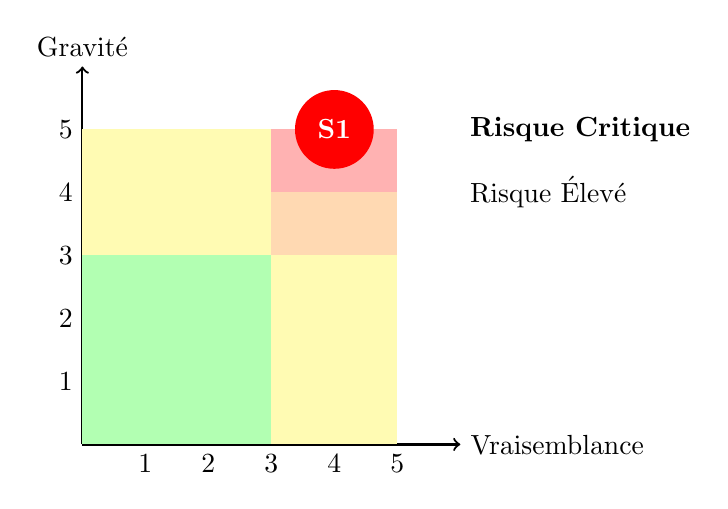
\begin{tikzpicture}[scale=0.8]
    % Axes
    \draw[thick,->] (0,0) -- (6,0) node[right] {Vraisemblance};
    \draw[thick,->] (0,0) -- (0,6) node[above] {Gravité};
    
    % Labels Axes
    \foreach \x in {1,...,5} {
        \node at (\x,0) [below] {\x};
        \node at (0,\x) [left] {\x};
    }
    
    % Zones de couleur
    \fill[green!30] (0,0) rectangle (3,3); % Faible
    \fill[yellow!30] (3,0) rectangle (5,3); % Moyen
    \fill[yellow!30] (0,3) rectangle (3,5); % Moyen
    \fill[orange!30] (3,3) rectangle (5,4); % Elevé
    \fill[orange!30] (4,3) rectangle (5,5); % Elevé
    \fill[red!30] (3,4) rectangle (5,5); % Critique
    
    % Le risque LiZbiZ
    \node[circle, fill=red, text=white, minimum size=1cm] at (4,5) {\textbf{S1}};
    
    % Légende
    \node[right] at (6,5) {\textbf{Risque Critique}};
    \node[right] at (6,4) {Risque Élevé};
\end{tikzpicture}
\caption{Positionnement du risque Ransomware chez LiZbiZ}
\end{figure}

% ------------------------------------------------------------------------------
\section{Travaux Pratiques : Première Mission}
% ------------------------------------------------------------------------------

\begin{boxlizbiz}
\textbf{Mission pour les étudiants :}

En utilisant le laboratoire GNS3 et les éléments fournis :
\begin{enumerate}
    \item Complétez la fiche de risque EBIOS pour le scénario S1.
    \item Identifiez un second scénario de risque concernant le \textbf{WiFi Logistique} (Indice : quel actif est sensible ? Quelle menace ?).
    \item Proposez une première mesure de réduction simple pour faire baisser la vraisemblance du scénario Ransomware.
\end{enumerate}
\end{boxlizbiz}

% ==============================================================================
% Fichier : 02_module_risque.tex (Extrait Chapitre 5)
% Description : Traitement du Risque et Reporting
% ==============================================================================
\chapter{Traitement du Risque et Reporting}
\label{chap:traitement}

Une fois les risques identifiés et analysés, l'entreprise doit décider d'une stratégie. C'est ici que la cybersécurité rejoint la gestion de projet et la finance.

\section{Les 4 Options de Traitement du Risque}

La norme ISO 27005 définit quatre options principales pour traiter un risque. Le choix dépend de l'appétence au risque de l'entreprise et du rapport coût/bénéfice.

\subsection{Option 1 : Réduction (Mitigation)}

\begin{boxdef}
\textbf{Réduction :} Mettre en place des mesures de sécurité (techniques ou organisationnelles) pour diminuer la Probabilité et/ou la Gravité du risque. C'est l'option la plus courante.
\end{boxdef}

\begin{boxlizbiz}
\textbf{LiZbiZ (Risque Ransomware) :}
Installer un système de sauvegarde externalisé et cloisonner le réseau (segmentation VLAN).
\textbf{Effet :} La Gravité baisse (on peut restaurer) et la Probabilité baisse (plus difficile à propager).
\end{boxlizbiz}

\subsection{Option 2 : Acceptation}

\begin{boxdef}
\textbf{Acceptation :} Décider consciemment de ne pas traiter le risque. Cela s'applique généralement aux risques faibles ou lorsque le coût du traitement dépasse le coût de l'impact potentiel.
\end{boxdef}

\begin{boxlizbiz}
\textbf{LiZbiZ :} Un risque de panne mineure d'une imprimante du service marketing (impact faible) peut être accepté. On ne mettra pas d'imprimante de secours.
\end{boxlizbiz}

\subsection{Option 3 : Évitement (Suppression)}

\begin{boxdef}
\textbf{Évitement :} Supprimer l'activité ou l'actif qui génère le risque. C'est une décision radicale.
\end{boxdef}

\begin{boxlizbiz}
\textbf{LiZbiZ :} Si la vente d'un produit spécifique (ex: kits de survie) génère trop de fraudes et de risques légaux, LiZbiZ peut décider d'arrêter purement et simplement cette gamme de produits. Le risque disparaît, mais le chiffre d'affaires aussi.
\end{boxlizbiz}

\subsection{Option 4 : Transfert (Partage)}

\begin{boxdef}
\textbf{Transfert :} Déplacer l'impact financier du risque vers un tiers. Cela se fait généralement par le biais d'une assurance ou de l'externalisation.
\end{boxdef}

\begin{boxlizbiz}
\textbf{LiZbiZ :} Souscrire une assurance "Cyber-risque" pour couvrir les frais de rançon et de communication de crise. Ou externaliser l'hébergement du site web à un Cloud Provider (AWS/Azure) pour transférer le risque physique du serveur.
\end{boxlizbiz}

% ------------------------------------------------------------------------------
\section{Le Plan d'Action Sécurité (PAS)}
% ------------------------------------------------------------------------------

\subsection{Définition}

\begin{boxdef}
\textbf{PAS (Plan d'Action Sécurité) :} Document opérationnel qui liste les mesures décidées, les responsables, les budgets et les échéances pour traiter les risques identifiés. C'est la "Feuille de route" du RSSI.
\end{boxdef}

\subsection{Structure type d'un PAS}

Il doit être SMART (Spécifique, Mesurable, Atteignable, Réaliste, Temporel).

\begin{table}[htbp]
\centering
\small
\begin{tabular}{p{4cm}p{2.5cm}p{2.5cm}p{2cm}p{2cm}}
    \toprule
    \textbf{Action} & \textbf{Responsable} & \textbf{Échéance} & \textbf{Budget} & \textbf{Priorité} \\
    \midrule
    Segmentation VLAN (Firewall) & Admin Sys & M+1 & 0€ (Interne) & Haute \\
    Mise à jour Serveur Web & Admin Sys & Immédiat & 0€ & Critique \\
    Formation anti-phishing & RH / RSSI & M+3 & 5000€ & Moyenne \\
    Souscription Assurance & DAF & M+2 & 10k€/an & Moyenne \\
    \bottomrule
\end{tabular}
\caption{Extrait du PAS pour LiZbiZ}
\end{table}

% ------------------------------------------------------------------------------
\section{Reporting et Argumentation Financière}
% ------------------------------------------------------------------------------

Le RSSI doit convaincre le COMEX de financer le PAS. Pour cela, il doit parler le langage de la direction.

\subsection{Le ROI de la Sécurité (ROSPI)}

Il est difficile de calculer un Retour sur Investissement (ROI) classique pour la sécurité, car la sécurité "ne rapporte" pas d'argent direct, elle évite des pertes. On parle plutôt de \textbf{ROSPI} (Return On Security Investment).

\begin{boxdef}
\textbf{ROSPI :} Comparaison entre le coût de la mesure et l'économie de perte potentielle (ALE).
\[ ROSPI = \frac{(Perte\_Évitée - Coût\_Mesure)}{Coût\_Mesure} \]
\end{boxdef}

\subsection{Argumentaire pour le COMEX}

Pour le risque Ransomware (Scénario S1) chez LiZbiZ :

\begin{itemize}
    \item \textbf{Coût de l'incident (Impact) :} 200 000 € (Perte CA + Amende + Image).
    \item \textbf{Probabilité annuelle :} 1 fois par an (Vraisemblance élevée).
    \item \textbf{Coût de la mesure (Segmentation) :} 5 000 € (Jours hommes).
    \item \textbf{Efficacité de la mesure :} Réduit la probabilité de 90\%.
\end{itemize}

\textbf{Calcul simplifié :}
Même si le calcul exact est complexe, l'argument est simple : "Investir 5 000 € maintenant évite un risque de perte de 200 000 € avec une probabilité très forte. C'est une assurance-vie pour l'entreprise."

% ------------------------------------------------------------------------------
\section{Cas LiZbiZ : Présentation au COMEX}
% ------------------------------------------------------------------------------

\subsection{Simulation}

Le DSI et le consultant (étudiant) présentent les résultats au COMEX (le professeur).

\begin{boxlizbiz}
\textbf{Scénario :} Le PDG de LiZbiZ hésite à valider le budget pour la segmentation réseau.

\textbf{Argument du Consultant :}
"Monsieur le PDG, notre analyse EBIOS montre que votre système de facturation est exposé à un risque critique. Actuellement, un pirate peut accéder aux données bancaires des clients depuis le site web public. Le coût de l'aménagement réseau est de 5 jours de travail. Le coût d'une fuite de données est estimé à 200k€ d'amendes RGPD et une perte de crédibilité boursière. Nous recommandons le traitement par \textbf{Réduction} immédiate."
\end{boxlizbiz}

% ------------------------------------------------------------------------------
\section{Exercices de Fin de Module}
% ------------------------------------------------------------------------------

\subsection{Exercice 1 : Décision de Traitement}

Pour chacun des risques suivants chez LiZbiZ, choisissez l'option de traitement la plus adaptée et justifiez :
\begin{enumerate}
    \item Risque de panne électrique générale du petit local serveur (Probabilité Faible, Gravité Haute).
    \item Risque de vol d'un smartphone d'un commercial (Probabilité Moyenne, Gravité Faible si données chiffrées).
    \item Risque juridique lié à l'utilisation d'un logiciel piraté sur un poste isolé.
\end{enumerate}

\subsection{Exercice 2 : Projet Final}

Rédigez une "Fiche de Risque" complète pour le scénario "Vol de données clients via le WiFi Logistique" et proposez un PAS de 3 actions concrètes.
% ==============================================================================
% Fichier : 02_module_risque.tex (Extrait Chapitre 6)
% Description : Evaluation du Module 1
% ==============================================================================
\chapter{Évaluation du Module 1}
\label{chap:evalmod1}

Cette évaluation valide l'acquisition des compétences liées à la gouvernance, l'analyse de risque et la prise de décision. Elle se décompose en trois parties : QCM, questions de synthèse et mise en situation pratique.

% ------------------------------------------------------------------------------
\section{Partie A : QCM (25 Questions)}
% ------------------------------------------------------------------------------

\textbf{Consigne :} Cochez la ou les bonnes réponses.

\begin{enumerate}
    \item La gouvernance du SI consiste principalement à :
    \begin{itemize}
        \item[A.] Installer des pare-feux.
        \item[B.] Définir les objectifs stratégiques et piloter la performance.
        \item[C.] Réparer les pannes informatiques.
        \item[D.] Programmer des applications métiers.
    \end{itemize}

    \item Dans une matrice RACI, qui est la personne qui "rend des comptes" et valide le résultat ?
    \begin{itemize}
        \item[A.] Responsible.
        \item[B.] Accountable.
        \item[C.] Consulted.
        \item[D.] Informed.
    \end{itemize}

    \item Quelle norme internationale traite spécifiquement de la gestion des risques en sécurité de l'information ?
    \begin{itemize}
        \item[A.] ISO 9001.
        \item[B.] ISO 27005.
        \item[C.] ISO 22301.
        \item[D.] ISO 26000.
    \end{itemize}

    \item Un "Actif" dans une analyse de risque est :
    \begin{itemize}
        \item[A.] Un logiciel de sécurité.
        \item[B.] Une ressource qui a de la valeur pour l'organisation.
        \item[C.] Un piratage informatique.
        \item[D.] Une norme obligatoire.
    \end{itemize}

    \item La formule de la Criticité est :
    \begin{itemize}
        \item[A.] Probabilité + Gravité.
        \item[B.] Probabilité $\times$ Gravité.
        \item[C.] Coût $\times$ Temps.
        \item[D.] Menace + Vulnérabilité.
    \end{itemize}

    \item Le risque résiduel est :
    \begin{itemize}
        \item[A.] Le risque avant toute mesure de protection.
        \item[B.] Le risque qui reste après application des mesures.
        \item[C.] Un risque qui ne peut jamais arriver.
        \item[D.] Un risque transféré à une assurance.
    \end{itemize}

    \item La méthode d'analyse de risque développée par l'ANSSI (France) s'appelle :
    \begin{itemize}
        \item[A.] NIST SP 800-30.
        \item[B.] OCTAVE.
        \item[C.] EBIOS RM.
        \item[D.] MEHARI.
    \end{itemize}

    \item Décider de ne pas héberger un service sensible pour ne pas prendre de risque est une stratégie de :
    \begin{itemize}
        \item[A.] Réduction.
        \item[B.] Acceptation.
        \item[C.] Transfert.
        \item[D.] Évitement.
    \end{itemize}

    \item Le RSSI est l'acronyme de :
    \begin{itemize}
        \item[A.] Responsable de la Sécurité des Systèmes d'Information.
        \item[B.] Réseau de Sécurité des Systèmes Informatiques.
        \item[C.] Responsable des Systèmes et Services Informatiques.
        \item[D.] Responsable Sécurité et Sureté Industrielle.
    \end{itemize}

    \item Une vulnérabilité est :
    \begin{itemize}
        \item[A.] Un actif critique.
        \item[B.] Une faiblesse pouvant être exploitée.
        \item[C.] Une attaque informatique.
        \item[D.] Un pare-feu désactivé.
    \end{itemize}

    \item Le DPO (Data Protection Officer) est principalement chargé de veiller au respect de :
    \begin{itemize}
        \item[A.] La loi de finances.
        \item[B.] Le RGPD.
        \item[C.] La sécurité physique.
        \item[D.] La comptabilité.
    \end{itemize}

    \item Dans EBIOS RM, l'atelier qui permet d'identifier les actifs essentiels est l'atelier :
    \begin{itemize}
        \item[A.] 1 (Contexte).
        \item[B.] 2 (Événements redoutés).
        \item[C.] 3 (Scénarios).
        \item[D.] 5 (Traitement).
    \end{itemize}

    \item Le triangle du risque est composé de :
    \begin{itemize}
        \item[A.] Actif, Menace, Vulnérabilité.
        \item[B.] Feu, Eau, Terre.
        \item[C.] Probabilité, Gravité, Coût.
        \item[D.] Hardware, Software, Humanware.
    \end{itemize}

    \item Souscrire une assurance cyber-risque est une stratégie de :
    \begin{itemize}
        \item[A.] Réduction.
        \item[B.] Acceptation.
        \item[C.] Transfert.
        \item[D.] Évitement.
    \end{itemize}

    \item L'alignement stratégique signifie que :
    \begin{itemize}
        \item[A.] La sécurité soutient les objectifs métier.
        \item[B.] Le métier obéit à la sécurité.
        \item[C.] La sécurité n'a pas de budget.
        \item[D.] L'IT et le Métier sont en conflit.
    \end{itemize}

    \item Le RACI est un outil de :
    \begin{itemize}
        \item[A.] Hacking.
        \item[B.] Répartition des rôles.
        \item[C.] Cryptographie.
        \item[D.] Développement logiciel.
    \end{itemize}

    \item La gravité d'un risque mesure :
    \begin{itemize}
        \item[A.] La chance qu'il se produise.
        \item[B.] L'ampleur des dommages s'il se produit.
        \item[C.] Le coût de la protection.
        \item[D.] La durée de l'attaque.
    \end{itemize}

    \item Le "COMEX" est :
    \begin{itemize}
        \item[A.] Un logiciel de gestion de mot de passe.
        \item[B.] Le Comité Exécutif de l'entreprise.
        \item[C.] Une norme ISO.
        \item[D.] Un type de virus.
    \end{itemize}

    \item Le PAS (Plan d'Action Sécurité) contient :
    \begin{itemize}
        \item[A.] Des actions, des responsables et des échéances.
        \item[B.] Des codes sources.
        \item[C.] Des mots de passe.
        \item[D.] Des factures fournisseurs.
    \end{itemize}

    \item Une erreur humaine (ex: envoi d'un fichier au mauvais destinataire) est :
    \begin{itemize}
        \item[A.] Une menace environnementale.
        \item[B.] Une menace humaine intentionnelle.
        \item[C.] Une menace humaine involontaire.
        \item[D.] Une vulnérabilité physique.
    \end{itemize}

    \item L'ISO 27001 concerne :
    \begin{itemize}
        \item[A.] La gestion de projet.
        \item[B.] Les exigences pour un SMSI (Système de Management de la Sécurité de l'Information).
        \item[C.] La qualité des logiciels.
        \item[D.] La continuité environnementale.
    \end{itemize}

    \item Le ROSPI (Return On Security Investment) mesure :
    \begin{itemize}
        \item[A.] La rentabilité financière de l'investissement sécurité.
        \item[B.] Le nombre d'attaques bloquées.
        \item[C.] La vitesse du réseau.
        \item[D.] La satisfaction utilisateur.
    \end{itemize}

    \item Un événement redouté concerne toujours l'impact sur :
    \begin{itemize}
        \item[A.] Le support technique.
        \item[B.] L'actif essentiel (Métier).
        \item[C.] Le budget.
        \item[D.] Le fournisseur.
    \end{itemize}

    \item Accepter un risque est justifié si :
    \begin{itemize}
        \item[A.] Le coût du traitement dépasse le coût de l'impact.
        \item[B.] La direction refuse tout budget.
        \item[C.] Le risque est critique.
        \item[D.] Le RSSI est absent.
    \end{itemize}

    \item Le cycle PDCA signifie :
    \begin{itemize}
        \item[A.] Plan, Do, Check, Act.
        \item[B.] Protect, Detect, Correct, Analyse.
        \item[C.] Plan, Deploy, Control, Audit.
        \item[D.] Program, Develop, Compute, Apply.
    \end{itemize}
\end{enumerate}

% ------------------------------------------------------------------------------
\section{Partie B : Questions Ouvertes (10 Questions)}
% ------------------------------------------------------------------------------

\textbf{Consigne :} Répondez de manière synthétique (5-10 lignes par question).

\begin{enumerate}
    \item Expliquez la différence fondamentale entre "Gouvernance" et "Management" dans le contexte de la cybersécurité.
    \item Pourquoi le RSSI ne doit-il pas être rattaché hiérarchiquement à la DSI ? Quel est le risque de conflit d'intérêts ?
    \item Définissez les termes "Actif", "Menace" et "Vulnérabilité" et donnez un exemple concret pour chacun dans un contexte de banque en ligne.
    \item Quelle est la différence entre le "Risque Inhérent" et le "Risque Résiduel" ?
    \item Pourquoi la méthode EBIOS RM est-elle particulièrement adaptée aux entreprises françaises ?
    \item Expliquez le rôle du "Accountable" dans une matrice RACI. Pourquoi est-il unique pour chaque tâche ?
    \item Citez les quatre options de traitement du risque et donnez un exemple pour chacune dans le contexte d'un risque de vol d'ordinateur portable.
    \item Qu'est-ce que le ROSPI et pourquoi est-il utile pour convaincre le COMEX ?
    \item Décrivez les critères D.I.C.T (Disponibilité, Intégrité, Confidentialité, Traçabilité) avec un exemple pour chacun.
    \item À quoi sert un Plan d'Action Sécurité (PAS) ? Quels sont ses éléments constitutifs minimums ?
\end{enumerate}

% ------------------------------------------------------------------------------
\section{Partie C : Cas Pratique - Mise en Condition (TP)}
% ------------------------------------------------------------------------------

\subsection{Scénario : La Menace Interne}

\begin{boxlizbiz}
\textbf{Contexte :}
Nous sommes 3 mois après votre première mission. Le projet de segmentation réseau est validé. Cependant, ce matin, la DSI de LiZbiZ vous appelle en urgence.

\textbf{Situation :} Un ancien développeur, parti en mauvais termes la semaine dernière, a tenté d'accéder au serveur de code source hier soir. Son compte n'avait pas été désactivé. L'alerte a été levée par le système de détection (SIEM), mais l'intrusion a échoué de justesse car le mot de passe du serveur était complexe.

Le Directeur Général est inquiet : "Si ce développeur avait réussi, il aurait pu voler notre code source ou insérer une porte dérobée !"
\end{boxlizbiz}

\subsection{Travaux à Réaliser}

Vous avez 1h30 pour produire un rapport complet (Format Libre : PDF, PowerPoint).

\textbf{Livrable 1 : Identification du Risque (Méthode EBIOS)}
\begin{itemize}
    \item Identifiez l'Actif Essentiel concerné.
    \item Identifiez la Menace (Source + Motivation).
    \item Identifiez la Vulnérabilité exploitée (citezen 2 failles : une humaine, une technique).
    \item Définissez l'Événement Redouté (Impact sur D.I.C.T).
\end{itemize}

\textbf{Livrable 2 : Estimation du Risque}
\begin{itemize}
    \item Proposez une Gravité (sur 5) et justifiez-la (Impact Business).
    \item Proposez une Probabilité (sur 5) et justifiez-la (Facilité).
    \item Calculez la Criticité et placez le risque sur une matrice.
\end{itemize}

\textbf{Livrable 3 : Plan d'Action (PAS)}
\begin{itemize}
    \item Proposez 3 mesures correctives immédiates pour réduire ce risque.
    \item Pour chaque mesure, indiquez l'option de traitement choisie (Réduction, Transfert, etc.).
    \item Définissez un RACI simple pour la mise en œuvre de ces mesures.
\end{itemize}

\textbf{Livrable 4 : Argumentaire Direction}
\begin{itemize}
    \item Rédigez un paragraphe de 5 lignes max à destination du PDG pour lui expliquer pourquoi ce risque, bien que l'attaque ait échoué, reste "Critique" et justifie des investissements immédiats.
\end{itemize}

% ==============================================================================
% Fichier : 03_module_audit.tex (Extrait Chapitre 1)
% Description : Introduction à l'Audit et au Management de la Qualité
% ==============================================================================

\clearpage
% ============================================================
% PARTIE II — Audit et Management de la Qualité
% ============================================================
\clearpage
\part{Audit et Management de la Qualité}

\chapter{Introduction à l'Audit et au Management de la Qualité}
\label{chap:introaudit}

Après avoir analysé les risques (Module 1), il faut vérifier si les mesures prises sont efficaces. C'est le rôle de l'audit. Ce chapitre pose les fondations de la démarche d'audit et de la qualité.

\section{Présentation : Qu'est-ce qu'un Audit ?}

\subsection{Définition de l'Audit}

\begin{boxdef}
\textbf{Audit :} Processus méthodique, indépendant et documenté permettant d'obtenir des preuves objectives et de les évaluer pour déterminer dans quelle mesure les critères d'audit sont satisfaits.
\end{boxdef}

Contrairement à une inspection "policière", l'audit est un outil de pilotage et d'amélioration continue. Il ne s'agit pas de punir, mais de mesurer l'écart entre ce qui est prévu (la règle) et ce qui est fait (la réalité).

\subsection{Les Trois Types d'Audits}

Il est crucial de distinguer les différents types d'audits selon l'auditeur et l'objectif.

\begin{table}[htbp]
\centering
\begin{tabular}{p{2.5cm}p{4cm}p{5cm}}
    \toprule
    \textbf{Type} & \textbf{Auditeur} & \textbf{Objectif} \\
    \midrule
    \textbf{Interne} & Membre de l'entreprise (ou prestataire mandaté par elle). & Vérifier l'efficacité interne, préparer une certification, améliorer les processus. \\
    \textbf{Externe (Tiers)} & Prestataire externe (Cabinet de conseil). & Certification (ISO 27001), conformité réglementaire, ou audit de fournisseurs. \\
    \textbf{De Conformité} & Régulateur (CNIL, Banque de France) ou Client. & Vérifier le respect d'une loi ou d'un contrat. \\
    \bottomrule
\end{tabular}
\caption{Typologie des audits}
\end{table}

\begin{boxlizbiz}
\textbf{Contexte LiZbiZ :}
L'entreprise reçoit de plus en plus de demandes de clients B2B : "Êtes-vous certifiés ISO 27001 ?". Le PDG décide de lancer un projet de certification.
\begin{itemize}
    \item \textbf{Audit Interne :} Vous (les étudiants) allez réaliser un pré-audit pour voir si LiZbiZ est prête.
    \item \textbf{Audit Externe :} Un organisme certificateur (ex: BSI, AFNOR) viendra dans 6 mois pour délivrer le certificat.
\end{itemize}
\end{boxlizbiz}

\subsection{La Notion de Qualité dans le SI}

L'audit est l'un des piliers du \textbf{Management de la Qualité}. La qualité en informatique, ce n'est pas seulement "un code sans bug", c'est la capacité du SI à satisfaire les besoins exprimés et implicites des utilisateurs.

\begin{boxdef}
\textbf{Qualité :} Aptitude d'un ensemble de caractéristiques intrinsèques à satisfaire les exigences (Norme ISO 9000).
\end{boxdef}

Lien avec la sécurité : Un SI de "qualité" est un SI sécurisé, disponible et conforme.

% ------------------------------------------------------------------------------
\section{Concepts Clés de l'Audit}
% ------------------------------------------------------------------------------

\subsection{Indépendance de l'Auditeur}

C'est le principe fondamental. L'auditeur ne doit pas être juge et partie.

\begin{boxalert}
\textbf{Règle absolue :} On n'audite jamais son propre travail. Si l'administrateur réseau vérifie ses propres configurations, ce n'est pas un audit, c'est un autocontrôle.
\end{boxalert}

\begin{boxlizbiz}
\textbf{Erreur classique chez LiZbiZ :}
La DSI (Sophie) voulait demander à l'Admin Sys de vérifier la sécurité du pare-feu. C'est impossible car c'est lui qui configure le pare-feu.
\textbf{Solution :} Vous (consultants externes) ou un autre technicien non responsable du pare-feu devez effectuer l'audit.
\end{boxlizbiz}

\subsection{Objectivité et Preuves}

L'audit se base sur des \textbf{preuves} (évidences), jamais sur des suppositions.

\textbf{Sources de preuves :}
\begin{itemize}
    \item \textbf{Documents :} Procédures écrites, politiques de sécurité, tickets d'incident.
    \item \textbf{Enregistrements :} Logs système, sauvegardes, captures d'écran.
    \item \textbf{Entretiens :} Témoignages des collaborateurs (recoupés avec les écrits).
    \item \textbf{Observation :} Voir ce qui se passe réellement (ex: mots de passe sur des post-it).
\end{itemize}

\subsection{Critères d'Audit}

\begin{boxdef}
\textbf{Critères d'audit :} L'ensemble des politiques, procédures ou exigences utilisées comme référence. C'est le "mètre étalon".
\end{boxdef}

Exemple de critères : "La politique de sécurité de LiZbiZ", "La norme ISO 27001", "Le RGPD".

% ------------------------------------------------------------------------------
\section{Jargon et Vocabulaire de l'Auditeur}
% ------------------------------------------------------------------------------

\subsection{Les Acteurs de l'Audit}

\begin{itemize}
    \item \textbf{L'Auditeur :} Celui qui mène l'audit.
    \item \textbf{L'Audité :} La personne ou l'entité qui est auditée (ex: le service informatique).
    \item \textbf{Le Commanditaire :} Celui qui demande l'audit (ex: le PDG ou le COMEX).
    \item \textbf{Le Guide :} Personne désignée par l'audité pour accompagner l'auditeur (ex: le DSI).
\end{itemize}

\subsection{Le Périmètre d'Audit (Scope)}

C'est la frontière de l'audit. Il est impossible de tout auditer en une fois. Le périmètre définit ce qui est \textbf{in} et ce qui est \textbf{out}.

\begin{boxlizbiz}
\textbf{Périmètre LiZbiZ (Projet Certification) :}
\begin{itemize}
    \item \textbf{IN :} Le système d'information de gestion des commandes (ERP, Web, DB), les locaux de Lyon.
    \item \textbf{OUT :} La logistique de transport externalisée (sous-traitant), le site de test de développement.
\end{itemize}
\end{boxlizbiz}

\subsection{La Non-Conformité (NC)}

C'est le résultat final de l'audit le plus redouté.

\begin{boxdef}
\textbf{Non-Conformité (NC) :} Non-satisfaction d'une exigence. C'est l'écart entre le "Dire" (la procédure) et le "Faire" (la réalité), ou l'absence de procédure pour une exigence obligatoire.
\end{boxdef}

On distingue souvent :
\begin{itemize}
    \item \textbf{NC Majeure :} Défaillance grave ou absence totale de système. Bloque la certification.
    \item \textbf{NC Mineure :} Incident isolé ou petite erreur documentaire. N'empêche pas la certification si corrigée.
    \item \textbf{Observation :} Piste d'amélioration, pas encore une non-conformité.
\end{itemize}

% ------------------------------------------------------------------------------
\section{Cas LiZbiZ : Préparation de la Mission d'Audit}
% ------------------------------------------------------------------------------

\subsection{Contexte de la Mission}

Le PDG de LiZbiZ veut obtenir la certification ISO 27001 d'ici un an. Il mandate votre cabinet de conseil pour réaliser un \textbf{audit de pré-évaluation (Gap Analysis)}.

\subsection{Objectifs}

L'objectif n'est pas de "piéger" les équipes, mais d'identifier les écarts avant le passage du certificateur officiel.

\subsection{Rôles (RACI de l'Audit)}

\begin{table}[htbp]
\centering
\begin{tabular}{lcccc}
    \toprule
    \textbf{Tâche} & \textbf{PDG} & \textbf{DSI} & \textbf{Équipe IT} & \textbf{Vous (Auditeurs)} \\
    \midrule
    Définir le périmètre & A & C & I & C \\
    Préparer les documents & I & A & R & I \\
    Réaliser les tests techniques & I & I & C & R \\
    Rédiger le rapport d'audit & I & I & I & A \\
    Présenter les résultats & I & I & I & R \\
    \bottomrule
\end{tabular}
\caption{RACI de la mission d'audit LiZbiZ}
\end{table}

\subsection{Travaux Pratiques : Préparation}

\begin{boxlizbiz}
\textbf{Exercice de préparation :}
Avant de commencer les tests techniques, vous devez préparer votre grille d'audit.
À partir de l'Annexe A de l'ISO 27001, sélectionnez 3 contrôles (ex: A.9.2.1 Enregistrement des utilisateurs) qui seront audités en priorité pour la séance suivante.
\end{boxlizbiz}

% ==============================================================================
% Fichier : 03_module_audit.tex (Extrait Chapitre 2)
% Description : Le Processus d'Audit selon ISO 19011
% ==============================================================================
\chapter{Le Processus d'Audit (ISO 19011)}
\label{chap:procaudita}

La norme \textbf{ISO 19011} fournit les lignes directrices pour auditer les systèmes de management. C'est la "bible" de l'auditeur, décrivant étape par étape comment mener une mission.

\section{Présentation de l'ISO 19011}

\subsection{Définition et Champ d'Application}

\begin{boxdef}
\textbf{ISO 19011} : Norme internationale intitulée "Lignes directrices pour l'audit des systèmes de management". Elle s'applique à tous les types d'audits (Qualité ISO 9001, Sécurité ISO 27001, Environnement ISO 14001, etc.).
\end{boxdef}

Elle définit les principes d'audit (Intégrité, Présentation équitable, Devoir de vigilance, Confidentialité, Indépendance, Approche fondée sur la preuve) et le processus complet.

\subsection{Vue d'ensemble du Processus}

Le processus d'audit est cyclique. La norme (Section 6) le divise en plusieurs phases séquentielles :
\begin{enumerate}
    \item Déclenchement de l'audit.
    \item Préparation des activités d'audit.
    \item Réalisation des activités d'audit.
    \item Préparation et distribution du rapport.
    \item Clôture et suivi.
\end{enumerate}

% ------------------------------------------------------------------------------
\section{Phase 1 : Déclenchement de l'Audit (ISO 19011, Section 6.2)}
% ------------------------------------------------------------------------------

Cette phase est administrative mais cruciale pour cadrer la mission.

\subsection{Établissement du contact initial}

L'auditeur rencontre le commanditaire pour définir les objectifs.

\begin{boxlizbiz}
\textbf{LiZbiZ :} Le commanditaire est le PDG. L'objectif n'est pas de "piéger la DSI", mais de "mesurer l'écart par rapport à l'ISO 27001" pour préparer la certification.
\end{boxlizbiz}

\subsection{Détermination de la faisabilité}

L'auditeur vérifie s'il a les ressources nécessaires :
\begin{itemize}
    \item Accès aux documents ?
    \item Disponibilité du personnel clé ?
    \item Temps imparti suffisant ?
\end{itemize}

\subsection{Constitution de l'équipe d'audit}

Pour LiZbiZ, l'équipe sera constituée d'un \textbf{Auditeur Principal} (l'étudiant chef de projet) et d'\textbf{Auditeurs Techniques} (les autres étudiants).

% ------------------------------------------------------------------------------
\section{Phase 2 : Préparation de l'Audit (ISO 19011, Section 6.3)}
% ------------------------------------------------------------------------------

C'est le travail "de bureau" avant d'aller sur le terrain.

\subsection{Revue documentaire (Pré-audit)}

L'auditeur lit les documents existants pour préparer sa grille de vérification.

\begin{boxlizbiz}
\textbf{LiZbiZ :} Vous demandez à consulter la "Politique de Sécurité" et "La procédure de gestion des accès". Si ces documents n'existent pas, c'est déjà une Non-Conformité potentielle identifiée avant même de commencer.
\end{boxlizbiz}

\subsection{Plan d'Audit (Audit Plan)}

C'est le document contractuel validé par l'audité. Il précise le "Qui, Quoi, Où, Quand".

\begin{table}[htbp]
\centering
\small
\begin{tabular}{|p{3cm}|p{3cm}|p{3cm}|p{3cm}|}
    \hline
    \textbf{Date / Heure} & \textbf{Activité} & \textbf{Auditeur} & \textbf{Audité} \\
    \hline
    09h00 - 09h30 & Réunion d'ouverture & Chef d'équipe & DSI + Equipe \\
    \hline
    09h30 - 11h00 & Audit technique (Pare-feu, Logs) & Auditeur Tech & Admin Sys \\
    \hline
    11h00 - 12h30 & Audit organisationnel (RH) & Auditeur Orga & DRH \\
    \hline
    14h00 - 15h00 & Synthèse équipe & Équipe complète & - \\
    \hline
    15h00 - 16h00 & Réunion de clôture & Chef d'équipe & DSI + PDG \\
    \hline
\end{tabular}
\caption{Extrait du Plan d'Audit LiZbiZ}
\end{table}

\subsection{Feuille de Route (Checklist)}

C'est l'outil de travail de l'auditeur sur le terrain. Elle liste les questions à poser et les points à vérifier.

\begin{boxdef}
\textbf{Checklist (Feuille de route) :} Document détaillé traduisant les exigences de la norme (ex: ISO 27001) en questions fermées ou ouvertes.
\end{boxdef}

Exemple de checklist pour l'ISO 27001 Annexe A.9 (Contrôle d'accès) :
\begin{itemize}
    \item \textit{Question :} "Montrez-moi la liste des utilisateurs ayant des privilèges administrateurs."
    \item \textit{Question :} "Comment procédez-vous lors du départ d'un collaborateur ?"
\end{itemize}

% ------------------------------------------------------------------------------
\section{Phase 3 : Réalisation de l'Audit (ISO 19011, Section 6.4)}
% ------------------------------------------------------------------------------

C'est le moment de la vérité, sur le terrain (ou dans le lab GNS3).

\subsection{Réunion d'Ouverture (Opening Meeting)}

C'est une réunion formelle pour confirmer le plan.
\textbf{Ordre du jour type :}
\begin{itemize}
    \item Présentation des participants.
    \item Rappel du périmètre et des objectifs.
    \item Confirmation des ressources et accès.
    \item Rappel des règles de confidentialité.
\end{itemize}

\subsection{Collecte et Vérification des Informations}

L'auditeur collecte des preuves par trois moyens (Technique des 3 "E") :
\begin{enumerate}
    \item \textbf{Entretiens :} Questionner le personnel.
    \item \textbf{Examen documentaire :} Lire les procédures, regarder les logs.
    \item \textbf{Observation :} Regarder les activités réelles (ex: voir si l'écran est verrouillé).
\end{enumerate}

\begin{boxalert}
\textbf{Règle de l'échantillonnage :} L'auditeur ne peut pas tout vérifier. Il sélectionne des échantillons (ex: 5 comptes utilisateurs au hasard sur 100). Si 2 sur 5 sont mal gérés, il conclura à une anomalie généralisée.
\end{boxalert}

\subsection{Réunion de Clôture (Closing Meeting)}

À la fin de l'audit, l'équipe présente ses conclusions à l'audité.
\begin{itemize}
    \item C'est un moment de communication délicate.
    \item On présente les constats (faits objectifs).
    \item On annonce les Non-Conformités (NC).
    \item On ne donne pas encore les recommandations (ce n'est pas le rôle de l'auditeur de faire le travail de l'audité, sauf audit interne conseil).
\end{itemize}

% ------------------------------------------------------------------------------
\section{Phase 4 et 5 : Rapport et Suivi (ISO 19011, Sections 6.5 à 6.7)}
% ------------------------------------------------------------------------------

\subsection{Le Rapport d'Audit}

Il doit être clair, complet et factuel. Il contient :
\begin{itemize}
    \item Le périmètre et les objectifs.
    \item Le déroulement de l'audit.
    \item Les conclusions (Forces, Faiblesses).
    \item Les Non-Conformités détaillées (Exigence non satisfaite + Preuve).
\end{itemize}

\subsection{Le Suivi (Follow-up)}

L'audit ne s'arrête pas au rapport. L'audité doit mettre en place des actions correctives. L'auditeur doit vérifier l'efficacité de ces actions (souvent lors d'un audit de suivi ultérieur).

% ------------------------------------------------------------------------------
\section{Cas LiZbiZ : Simulation des Réunions}
% ------------------------------------------------------------------------------

\subsection{Exercice de Simulation (Jeu de rôle)}

\begin{boxlizbiz}
\textbf{Mise en situation :}
Les étudiants se répartissent les rôles : Auditeurs vs Audités (DSI, Admin Sys, RH).

\textbf{Scénario Réunion d'Ouverture :}
Les auditeurs doivent présenter le plan d'audit. L'Admin Sys (joué par un étudiant) tente de refuser l'accès aux logs en disant "C'est trop sensible, vous allez casser le système".
\textbf{Réponse attendue :} L'auditeur doit rappeler le mandat du PDG et les règles de l'audit (non-modification du système).
\end{boxlizbiz}

% ==============================================================================
% Fichier : 03_module_audit.tex (Extrait Chapitre 2)
% Description : Le Processus d'Audit selon ISO 19011
% ==============================================================================
\input{chapitres/11_processus_audit_b}
\chapter{Référentiels et Critères d'Évaluation}
\label{chap:refaudit}

Un auditeur a besoin d'un "mètre étalon" pour mesurer la conformité. Ce mètre est le \textbf{référentiel}. Sans référentiel, l'audit n'est qu'une simple opinion.

\section{La Structure Commune (High Level Structure)}
% ------------------------------------------------------------------------------

Depuis 2012, les normes de management (ISO 9001, ISO 27001, ISO 22301) partagent une structure commune pour faciliter leur intégration.

\begin{boxdef}
\textbf{High Level Structure (HLS) :} Structure identique en 10 chapitres pour toutes les normes ISO de management. Cela permet d'aligner Qualité, Sécurité et Environnement dans un Système de Management Intégré (SMI).
\end{boxdef}

Les chapitres 4 à 10 sont les chapitres "exigentiels" (ceux sur lesquels on audite) :
\begin{itemize}
    \item \textbf{Chapitre 4 :} Contexte de l'organisme.
    \item \textbf{Chapitre 5 :} Leadership (Engagement de la direction).
    \item \textbf{Chapitre 6 :} Planification (Analyse de risque).
    \item \textbf{Chapitre 7 :} Support (Ressources, Compétences, Sensibilisation).
    \item \textbf{Chapitre 8 :} Réalisation (Opérations, Plan d'action).
    \item \textbf{Chapitre 9 :} Évaluation des performances (Audit interne, Indicateurs).
    \item \textbf{Chapitre 10 :} Amélioration (Non-conformités, Actions correctives).
\end{itemize}

% ------------------------------------------------------------------------------
\section{ISO 27001 : La Référence Sécurité (SMSI)}
% ------------------------------------------------------------------------------

\subsection{Présentation}

\begin{boxdef}
\textbf{ISO 27001} : Norme internationale définissant les exigences pour établir, mettre en œuvre, maintenir et améliorer un Système de Management de la Sécurité de l'Information (SMSI).
\end{boxdef}

C'est la norme "système" : elle dit \textit{comment} manager la sécurité (PDCA).

\subsection{L'Annexe A : Mesures de Sécurité}

C'est la partie la plus connue des techniciens. L'Annexe A contient une liste de \textbf{mesures (contrôles)} à implémenter pour réduire les risques.

\begin{boxlizbiz}
\textbf{Structure de l'Annexe A (ISO 27001:2022) chez LiZbiZ :}
\begin{itemize}
    \item \textbf{A.5 :} Politiques de sécurité.
    \item \textbf{A.6 :} Organisation de la sécurité (Rôles RACI).
    \item \textbf{A.8 :} Sécurité liée aux ressources humaines (Embauche, Départ).
    \item \textbf{A.9 :} Contrôle d'accès (Mots de passe, Privilèges).
    \item \textbf{A.12 :} Sécurité des opérations (Logs, Sauvegardes, Malware).
\end{itemize}
\end{boxlizbiz}

\subsection{Notion d'Exigence vs Recommandation}

En audit, la nuance est importante :
\begin{itemize}
    \item \textbf{Exigence ("Shall") :} Obligatoire pour la certification.
    \item \textbf{Recommandation ("Should") :} Bonne pratique, mais non bloquante.
\end{itemize}

\begin{boxalert}
Dans l'ISO 27001, le corps de la norme contient des \textbf{exigences}. L'Annexe A contient des \textbf{mesures} qui sont obligatoires \textit{si} elles ont été sélectionnées dans la Déclaration d'Applicabilité (SOA - Statement of Applicability).
\end{boxalert}

% ------------------------------------------------------------------------------
\section{ISO 9001 : La Référence Qualité}
% ------------------------------------------------------------------------------

\subsection{Présentation}

\begin{boxdef}
\textbf{ISO 9001} : Norme internationale relative aux systèmes de management de la qualité. Elle vise la satisfaction du client et l'amélioration des processus.
\end{boxdef}

Pourquoi l'inclure dans un cours Cybersécurité ? Parce que la sécurité est un composant de la qualité de service.

\subsection{Approche Processus}

L'ISO 9001 exige que l'entreprise cartographie ses processus.
\begin{itemize}
    \item \textbf{Processus de Direction :} Pilotage.
    \item \textbf{Processus de Réalisation :} Création de valeur (Vente, Livraison).
    \item \textbf{Processus Support :} Support (RH, IT, Comptabilité).
\end{itemize}

\begin{boxlizbiz}
\textbf{Lien LiZbiZ :}
Un client commande un PC (Processus Réalisation). Si le SI est piraté et les données perdues, la qualité du service est dégradée. Auditer la qualité du processus "Livraison" implique de vérifier la disponibilité du SI.
\end{boxlizbiz}

% ------------------------------------------------------------------------------
\section{COBIT : La Référence Gouvernance IT}
% ------------------------------------------------------------------------------

\subsection{Présentation}

\begin{boxdef}
\textbf{COBIT} (Control Objectives for Information and Related Technologies) : Framework de bonnes pratiques pour la gouvernance et le management des SI, développé par l'ISACA.
\end{boxdef}

Contrairement à l'ISO 27001 (focus Sécurité), COBIT couvre tout le SI : stratégie, valeur, qualité, risque, sécurité.

\subsection{Les Domaines de COBIT}

COBIT divise le management de l'IT en 4 domaines principaux :
\begin{enumerate}
    \item \textbf{Planifier et Organiser (PO) :} Stratégie, Architecture.
    \item \textbf{Acquérir et Implémenter (AI) :} Projets, Développement.
    \item \textbf{Délivrer et Servir (DS) :} Exploitation, Support utilisateur, Sécurité.
    \item \textbf{Surveiller et Évaluer (ME) :} Audit, Performance, Conformité.
\end{enumerate}

\begin{boxlizbiz}
\textbf{Utilisation pour le Management (Filière Management SI) :}
L'auditeur utilise COBIT pour auditer la maturité de la DSI de LiZbiZ.
Exemple : Le processus "DS5 - Assurer la sécurité des services" de COBIT complète l'ISO 27001 en ajoutant une vision management (budget, rôles, indicateurs).
\end{boxlizbiz}

% ------------------------------------------------------------------------------
\section{Cas LiZbiZ : Sélection des Critères d'Audit}
% ------------------------------------------------------------------------------

\subsection{Déclaration d'Applicabilité (SOA)}

LiZbiZ ne peut pas (et ne doit pas) appliquer les 93 mesures de l'Annexe A de l'ISO 27001. L'entreprise doit rédiger une \textbf{Déclaration d'Applicabilité}.

\begin{boxdef}
\textbf{SOA (Statement of Applicability) :} Document listant les mesures de l'Annexe A ISO 27001 applicables à l'entreprise, avec une justification pour celles qui sont exclues.
\end{boxdef}

\subsection{Travaux Pratiques : Construction de la Grille d'Audit}

\begin{boxlizbiz}
\textbf{Mission :} Préparer la grille d'audit pour la section "Contrôle d'Accès".

En vous basant sur les risques identifiés dans le Module 1 (Risque Ransomware, Risque Interne), sélectionnez 4 mesures pertinentes de l'Annexe A de l'ISO 27001 pour LiZbiZ.

\textbf{Exemple de grille à construire :}
\begin{table}[htbp]
\centering
\small
\begin{tabular}{p{2cm}p{6cm}p{4cm}}
    \toprule
    \textbf{Référence} & \textbf{Exigence} & \textbf{Moyen de vérification (Audit)} \\
    \midrule
    A.5.15 & Contrôle des accès logiques. & Extraction AD, Test de robustesse mdp. \\
    A.5.16 & Gestion des identités. & Procédure écriture, Test départ salarié. \\
    A.8.2 & Privilèges d'accès. & Liste des "Admin", Vérification need-to-know. \\
    A.8.3 & Retrait des droits d'accès. & Comparatif liste salariés actifs vs comptes IT. \\
    \bottomrule
\end{tabular}
\end{table}
\end{boxlizbiz}

% ==============================================================================
% Fichier : 03_module_audit.tex (Extrait Chapitre 4)
% Description : Application Pratique - Réalisation de l'Audit LiZbiZ
% ==============================================================================
\chapter{Application Pratique : Réalisation de l'Audit LiZbiZ}
\label{chap:appaudit}

Ce chapitre met en œuvre les concepts théoriques sur le terrain. Nous simulons la phase de réalisation de l'audit (Section 6.4 de l'ISO 19011) au sein de l'entreprise LiZbiZ.

\section{Étape 1 : Collecte des Preuves}

L'auditeur doit collecter des informations vérifiables pour étayer ses conclusions.

\subsection{Les Trois Sources de Preuves}

\begin{enumerate}
    \item \textbf{Entretiens (Interviews) :} Échanges avec le personnel. (Subjectif, à recouper).
    \item \textbf{Observation :} Vue directe des activités. (Objectif, instant T).
    \item \textbf{Examen Documentaire et Technique :} Analyse de procédures, de logs, de configurations. (Objectif, historique).
\end{enumerate}

\begin{boxdef}
\textbf{Piste d'audit (Audit Trail) :} Enchaînement logique et documenté des preuves permettant de reconstituer l'historique d'un événement ou d'une transaction.
\end{boxdef}

\subsection{Technique de l'Échantillonnage}

Il est impossible de vérifier l'intégralité des logs ou des 150 comptes utilisateurs. L'auditeur pratique l'\textbf{échantillonnage}.

\begin{itemize}
    \item \textbf{Échantillonnage statistique :} Choix aléatoire de 10 comptes.
    \item \textbf{Échantillonnage orienté risque :} Choix ciblé (ex: les comptes admins, les nouveaux arrivés, les comptes inactifs depuis longtemps).
\end{itemize}

% ------------------------------------------------------------------------------
\section{Étape 2 : Audit Technique sur le Lab GNS3}
% ------------------------------------------------------------------------------

Nous connectons maintenant l'auditeur au laboratoire GNS3 de LiZbiZ pour un audit technique réel.

\subsection{Scénario 1 : Audit de la Segmentation Réseau}

\textbf{Critère d'audit (ISO 27001 - A.5.15) :} Le réseau doit être segmenté pour isoler les flux sensibles.

\begin{boxlizbiz}
\textbf{Mission Pratique :}
L'auditeur se connecte au routeur/firewall (pFsense) via la console.

\textbf{Tâche :} Vérifier les règles de filtrage inter-VLAN.
\textbf{Commande / Action :} Visualiser les règles (Access Control Lists).

\textbf{Constat attendu :}
L'auditeur découvre une règle "Allow Any -> Any" entre le VLAN 40 (IoT Logistique) et le VLAN 20 (Applicatif).
\textbf{Preuve :} Capture d'écran de la règle.
\textbf{Analyse :} Si un scanner IoT est compromis, il peut atteindre l'ERP. Non-respect du principe de moindre privilège.
\end{boxlizbiz}

\subsection{Scénario 2 : Audit des Droits d'Accès}

\textbf{Critère d'audit (ISO 27001 - A.5.18) :} Les droits d'accès doivent être révoqués lors du départ d'un employé.

\begin{boxlizbiz}
\textbf{Mission Pratique :}
L'auditeur accède au contrôleur de domaine (Windows Server AD).

\textbf{Tâche :} Lister les utilisateurs actifs et comparer avec la liste des employés fournie par la RH (document fictif "ListeEmployes\_Janvier.pdf").

\textbf{Constat attendu :}
L'auditeur trouve le compte "jmartin" actif. La liste RH indique que "Jean Martin" a quitté l'entreprise il y a 3 mois.
\textbf{Preuve :} Capture d'écran de l'Active Directory montrant "Enabled = True".
\textbf{Analyse :} Procédure de départ non appliquée. Risque de compte orphelin.
\end{boxlizbiz}

% ------------------------------------------------------------------------------
\section{Étape 3 : Audit Organisationnel (Jeu de Rôle)}
% ------------------------------------------------------------------------------

L'audit n'est pas que technique. Il faut auditer les processus humains.

\subsection{Scénario : Audit du Processus de Gestion des Incidents}

\textbf{Critère d'audit (ISO 27001 - A.5.24) :} L'organisation doit gérer les incidents de sécurité.

\begin{boxlizbiz}
\textbf{Mise en situation :}
L'auditeur interroge le Responsable Helpdesk (joué par un étudiant).

\textbf{Question de l'Auditeur :} "Que s'est-il passé le 12 janvier dernier suite à l'alerte antivirus sur le poste de la comptabilité ? Pouvez-vous me montrer le ticket ?"

\textbf{Réponse simulée (Erreur) :} "Ah, on a juste supprimé le virus. C'était un faux positif je pense, on n'a pas jugé utile d'ouvrir un ticket pour ça."

\textbf{Analyse de l'Auditeur :}
Absence de traceabilité. La procédure exige un ticket pour tout incident.
\end{boxlizbiz}

% ------------------------------------------------------------------------------
\section{Étape 4 : Analyse des Écarts et Formulation des Constats}
% ------------------------------------------------------------------------------

Une fois les preuves collectées, il faut formuler les constats.

\subsection{La Structure d'un Constat d'Audit}

Un bon constat répond à la structure : \textbf{Critère - Constat - Preuve - Cause - Risque}. Il ne doit jamais être une opinion.

\begin{table}[htbp]
\centering
\small
\begin{tabular}{p{3cm}p{9cm}}
    \toprule
    \textbf{Élément} & \textbf{Exemple LiZbiZ (Cas compte orphelin)} \\
    \midrule
    \textbf{Critère} & ISO 27001 A.5.18 : "Les droits d'accès doivent être retirés lors du départ". \\
    \textbf{Constat} & Le compte "jmartin" est toujours actif 3 mois après le départ. \\
    \textbf{Preuve} & Capture AD + Liste RH. \\
    \textbf{Cause} & Absence de communication fluide entre RH et IT. \\
    \textbf{Risque} & Utilisation malveillante des données par un ancien employé. \\
    \bottomrule
\end{tabular}
\caption{Formulation d'un constat d'audit}
\end{table}

\subsection{Classification de la Non-Conformité}

L'auditeur doit qualifier la gravité de l'écart.

\begin{itemize}
    \item \textbf{Non-Conformité Majeure :} Absence totale de système ou défaillance généralisée. (Ex: Aucune procédure de gestion des accès n'existe).
    \item \textbf{Non-Conformité Mineure :} Incident isolé, ponctuel. (Ex: Le compte "jmartin" est le seul oublié, la procédure existe mais a eu un raté).
    \item \textbf{Observation :} Piste d'amélioration, pas de non-respect strict. (Ex: La procédure de départ est sur papier, il serait mieux de la dématérialiser).
\end{itemize}

\begin{boxlizbiz}
\textbf{Décision pour LiZbiZ :}
L'oubli du compte "jmartin" est classé \textbf{Non-Conformité Mineure}, car la procédure existe. Cependant, si l'auditeur trouve 10 comptes orphelins sur 150, cela deviendra une \textbf{Non-Conformité Majeure} (défaillance du système de contrôle).
\end{boxlizbiz}

% ==============================================================================
% Fichier : 03_module_audit.tex (Extrait Chapitre 5)
% Description : Rapport d'Audit et Plan d'Actions Correctives
% ==============================================================================
\chapter{Rapport d'Audit et Plan d'Actions Correctives}
\label{chap:rapportaudit}

L'audit ne prend fin qu'avec la livraison du rapport et l'engagement de l'audité sur un plan d'action. C'est le moment de la vérité où les constats techniques se transforment en décisions managériales.

\section{La Réunion de Clôture (Closing Meeting)}
% ------------------------------------------------------------------------------

Avant de rédiger le rapport final, une réunion orale est obligatoire (ISO 19011, Section 6.4.9).

\subsection{Objectifs}

\begin{itemize}
    \item Présenter les conclusions et les non-conformités à l'audité.
    \item Clarifier les faits (pas les opinions).
    \item Confirmer le délai de remise du rapport officiel.
\end{itemize}

\subsection{Règle d'Or : Pas de Surprise}

L'audité ne doit pas découvrir une non-conformité majeure en lisant le rapport. Tout problème grave doit avoir été évoqué ou vu pendant l'audit.

\begin{boxlizbiz}
\textbf{Simulation LiZbiZ :}
Lors de la réunion de clôture, l'auditeur annonce : "Nous avons trouvé une non-conformité majeure sur la gestion des départs. 5 comptes sont actifs alors que les collaborateurs sont partis."
La DSI (Audité) confirme : "Oui, nous avons eu un bug de synchronisation avec les RH le mois dernier."
\end{boxlizbiz}

% ------------------------------------------------------------------------------
\section{Le Rapport d'Audit}
% ------------------------------------------------------------------------------

Le rapport est le livrable contractuel. Il doit être clair, concis et factuel.

\subsection{Structure Type du Rapport}

Le rapport suit généralement la structure suivante :

\begin{enumerate}
    \item \textbf{Page de Garde :} Référence, Date, Périmètre, Équipe.
    \item \textbf{Résumé à l'Attention de la Direction (Executive Summary) :} Note globale, risques majeurs en 1 page.
    \item \textbf{Objet et Périmètre :} Ce qui a été auditée (et ce qui ne l'a pas été).
    \item \textbf{Méthodologie :} Référentiel utilisé (ISO 27001), échantillonnage.
    \item \textbf{Synthèse des Constats :} Tableau récapitulatif des NC et Observations.
    \item \textbf{Détail des Non-Conformités :} Fiches détaillées (Critère, Preuve, Risque).
    \item \textbf{Conclusion et Recommandations :} Avis sur la capacité du système à atteindre les objectifs.
\end{enumerate}

\subsection{Qualité Rédactionnelle}

Un bon rapport d'audit doit être :
\begin{itemize}
    \item \textbf{Factuel :} "Le serveur n'a pas de pare-feu activé" (Vrai/Faux).
    \item \textbf{Non-jugemental :} Éviter "L'équipe est négligente". Préférer "La procédure de vérification n'est pas appliquée".
\end{itemize}

\subsection{Grille de Maturité (Optionnel)}

Pour les filières Management, on présente souvent les résultats sous forme de maturité (échelle 0 à 5), inspirée du modèle CMMI ou COBIT.

\begin{table}[htbp]
\centering
\begin{tabular}{cl}
    \toprule
    \textbf{Niveau} & \textbf{Description} \\
    \midrule
    0 & Inexistant (Pas de processus). \\
    1 & Initial (Processus chaotic, dépend des individus). \\
    2 & Reproductible (Processus défini mais pas formalisé). \\
    3 & Défini (Processus formalisé et documenté). \\
    4 & Maîtrisé (Processus mesuré par des indicateurs). \\
    5 & Optimisé (Amélioration continue automatisée). \\
    \bottomrule
\end{tabular}
\caption{Échelle de maturité simplifiée}
\end{table}

\begin{boxlizbiz}
\textbf{Résultat LiZbiZ :}
L'audit technique montre que la gestion des correctifs (Patch Management) est au \textbf{Niveau 1} (Initial) : "On met à jour quand on pense à le faire". L'objectif pour la certification est le \textbf{Niveau 3}.
\end{boxlizbiz}

% ------------------------------------------------------------------------------
\section{Le Plan d'Actions Correctives (PAC)}
% ------------------------------------------------------------------------------

Le rapport liste les problèmes, le PAC propose les solutions.

\subsection{Responsabilité}

L'auditeur identifie les problèmes, mais \textbf{l'audité est responsable} de la définition et de la mise en œuvre des actions correctives. L'auditeur ne doit pas "faire le travail" de l'audité, mais valider la pertinence du plan.

\subsection{Correction vs Action Corrective}

Il est vital de distinguer les deux concepts pour éviter la récurrence.

\begin{boxdef}
\begin{itemize}
    \item \textbf{Correction :} Action immédiate pour éliminer la non-conformité détectée (ex: Désactiver le compte "jmartin"). Soigne le symptôme.
    \item \textbf{Action Corrective :} Action pour éliminer la cause d'une non-conformité (ex: Mettre en place un export automatique hebdomadaire des départs RH vers l'IT). Empêche la récidive.
\end{itemize}
\end{boxdef}

\subsection{Structure du Plan d'Action}

\begin{table}[htbp]
\centering
\small
\begin{tabular}{p{3cm}p{4cm}p{2cm}p{2cm}}
    \toprule
    \textbf{NC Référence} & \textbf{Action Proposée} & \textbf{Responsable} & \textbf{Délai} \\
    \midrule
    NC-01 (Comptes orphelins) & \textbf{Correction :} Désactiver les 5 comptes. & Admin Sys & J+1 \\
    & \textbf{Action Corr :} Automatiser la revue des comptes. & DSI / DRH & J+30 \\
    \bottomrule
\end{tabular}
\caption{Exemple de Plan d'Actions Correctives pour LiZbiZ}
\end{table}

% ------------------------------------------------------------------------------
\section{Cas LiZbiZ : Présentation au COMEX}
% ------------------------------------------------------------------------------

\subsection{Le Scénario Final}

Le rapport est prêt. Le PDG de LiZbiZ convoque le COMEX pour écouter le verdict avant de signer les investissements.

\begin{boxlizbiz}
\textbf{Exercice de Synthèse (Oral ou Écrit) :}

Vous devez rédiger la page de synthèse (Executive Summary) du rapport d'audit LiZbiZ. Elle doit contenir :

\begin{enumerate}
    \item \textbf{L'avis global :} "Le SMSI de LiZbiZ est partiellement efficace. Non prêt pour la certification ISO 27001 sans mise à niveau."
    \item \textbf{Les points forts :} "Politique de sécurité rédigée, équipe technique compétente."
    \item \textbf{Les points critiques (Majeurs) :} "Absence de processus formalisé de gestion des départs (Sécurité Logique) et manque de visibilité sur les logs (Surveillance)."
    \item \textbf{La recommandation clé :} "Recrutement d'un RSSI dédié et mise en place d'un outil de gestion des identités (IAM) avant le 30 juin."
\end{enumerate}
\end{boxlizbiz}

% ==============================================================================
% Fichier : 03_module_audit.tex (Extrait Chapitre 6)
% Description : Evaluation du Module 2
% ==============================================================================
\chapter{Évaluation du Module 2}
\label{chap:evalmod2}

Cette évaluation valide les compétences liées à la méthodologie d'audit, la compréhension des référentiels (ISO 19011, 27001, 9001) et la capacité à rédiger un rapport professionnel.

% ------------------------------------------------------------------------------
\section{Partie A : QCM (25 Questions)}
% ------------------------------------------------------------------------------

\textbf{Consigne :} Cochez la ou les bonnes réponses.

\begin{enumerate}
    \item L'indépendance de l'auditeur signifie :
    \begin{itemize}
        \item[A.] Qu'il ne doit pas être ami avec l'audité.
        \item[B.] Qu'il ne doit pas être juge et partie (pas d'intérêt direct dans le résultat).
        \item[C.] Qu'il doit travailler seul.
        \item[D.] Qu'il doit être externe à l'entreprise.
    \end{itemize}

    \item La norme qui donne les lignes directrices pour réaliser un audit est :
    \begin{itemize}
        \item[A.] ISO 27001.
        \item[B.] ISO 19011.
        \item[C.] ISO 9001.
        \item[D.] ISO 27005.
    \end{itemize}

    \item Une "Non-Conformité Majeure" est :
    \begin{itemize}
        \item[A.] Un petit incident isolé.
        \item[B.] Une absence totale de système ou une défaillance généralisée.
        \item[C.] Une suggestion d'amélioration.
        \item[D.] Une mesure de sécurité non applicable.
    \end{itemize}

    \item La Déclaration d'Applicabilité (SOA) est un document lié à :
    \begin{itemize}
        \item[A.] L'ISO 9001.
        \item[B.] L'ISO 27001.
        \item[C.] L'ISO 19011.
        \item[D.] COBIT.
    \end{itemize}

    \item La "Correction" consiste à :
    \begin{itemize}
        \item[A.] Éliminer la cause du problème.
        \item[B.] Éliminer le problème immédiat (symptôme).
        \item[C.] Blâmer le responsable.
        \item[D.] Écrire une procédure.
    \end{itemize}

    \item Qui est le "Commanditaire" de l'audit ?
    \begin{itemize}
        \item[A.] La personne auditée.
        \item[B.] Celui qui demande et paie l'audit.
        \item[C.] L'auditeur principal.
        \item[D.] Le certificateur.
    \end{itemize}

    \item La "Réunion d'Ouverture" sert à :
    \begin{itemize}
        \item[A.] Présenter les résultats de l'audit.
        \item[B.] Confirmer le plan d'audit et les règles du jeu.
        \item[C.] Former les employés.
        \item[D.] Signer le certificat ISO.
    \end{itemize}

    \item L'Annexe A de l'ISO 27001 contient :
    \begin{itemize}
        \item[A.] Les exigences du système de management.
        \item[B.] La liste des mesures de sécurité (contrôles).
        \item[C.] Les procédures d'audit.
        \item[D.] La politique de sécurité type.
    \end{itemize}

    \item COBIT est un référentiel pour :
    \begin{itemize}
        \item[A.] La gouvernance et le management des SI.
        \item[B.] La qualité des logiciels uniquement.
        \item[C.] La gestion de projet.
        \item[D.] La sécurité physique.
    \end{itemize}

    \item Un constat d'audit doit contenir :
    \begin{itemize}
        \item[A.] Une opinion personnelle.
        \item[B.] Des faits, des preuves et une référence au critère.
        \item[C.] Une proposition de solution immédiate.
        \item[D.] Le nom du coupable.
    \end{itemize}

    \item La High Level Structure (HLS) permet :
    \begin{itemize}
        \item[A.] D'avoir une structure commune pour toutes les normes ISO de management.
        \item[B.] De mieux structurer le code informatique.
        \item[C.] De gérer la sécurité réseau.
        \item[D.] De hiérarchiser les employés.
    \end{itemize}

    \item L'échantillonnage en audit consiste à :
    \begin{itemize}
        \item[A.] Tout vérifier.
        \item[B.] Sélectionner une partie représentative pour tirer des conclusions.
        \item[C.] Choisir les meilleurs éléments.
        \item[D.] Ignorer les anomalies.
    \end{itemize}

    \item L'audit de certification est réalisé par :
    \begin{itemize}
        \item[A.] L'entreprise elle-même.
        \item[B.] Un organisme certificateur externe.
        \item[C.] Un client.
        \item[D.] Le syndicat.
    \end{itemize}

    \item Une "Action Corrective" vise à :
    \begin{itemize}
        \item[A.] Corriger l'erreur immédiatement.
        \item[B.] Empêcher l'erreur de se reproduire (traiter la cause).
        \item[C.] Punir l'employé.
        \item[D.] Transférer le risque.
    \end{itemize}

    \item ISO 9001 traite de :
    \begin{itemize}
        \item[A.] Sécurité de l'information.
        \item[B.] Management de la Qualité.
        \item[C.] Continuité d'activité.
        \item[D.] Protection des données personnelles.
    \end{itemize}

    \item La "Piste d'audit" (Audit Trail) est :
    \begin{itemize}
        \item[A.] Le chemin parcouru par l'auditeur dans les locaux.
        \item[B.] L'enchaînement de preuves permettant de reconstituer un événement.
        \item[C.] Le plan d'audit.
        \item[D.] La facture de l'audit.
    \end{itemize}

    \item Lors d'un entretien d'audit, l'auditeur doit :
    \begin{itemize}
        \item[A.] Poser des questions fermées (Oui/Non) uniquement.
        \item[B.] Poser des questions ouvertes (Comment, Pourquoi) et écouter.
        \item[C.] Donner son avis.
        \item[D.] Intimider l'audité pour obtenir des aveux.
    \end{itemize}

    \item Le rapport d'audit doit être remis :
    \begin{itemize}
        \item[A.] À l'audité uniquement.
        \item[B.] Au commanditaire.
        \item[C.] À la concurrence.
        \item[D.] Au gouvernement.
    \end{itemize}

    \item Un système de management est considéré "Mature" (Niveau 5 CMMI) si :
    \begin{itemize}
        \item[A.] Il n'existe pas.
        \item[B.] Il est en amélioration continue optimisée.
        \item[C.] Il est documenté.
        \item[D.] Il est géré par intuition.
    \end{itemize}

    \item Le PDCA (Plan-Do-Check-Act) est :
    \begin{itemize}
        \item[A.] Une méthode de hacking.
        \item[B.] Un cycle d'amélioration continue.
        \item[C.] Un type de pare-feu.
        \item[D.] Un logiciel de compta.
    \end{itemize}

    \item Si l'auditeur n'a pas accès aux documents demandés, c'est :
    \begin{itemize}
        \item[A.] Une observation.
        \item[B.] Une opportunité.
        \item[C.] Une non-conformité (entrave à l'audit).
        \item[D.] Un droit de l'audité.
    \end{itemize}

    \item La "Réunion de Clôture" se déroule :
    \begin{itemize}
        \item[A.] Avant l'audit.
        \item[B.] Au milieu de l'audit.
        \item[C.] À la fin de la phase terrain, avant le rapport final.
        \item[D.] Après la certification.
    \end{itemize}

    \item La "Checklist" est :
    \begin{itemize}
        \item[A.] La liste des courses de l'auditeur.
        \item[B.] La feuille de route listant les points à vérifier.
        \item[C.] Le rapport final.
        \item[D.] La liste des non-conformités.
    \end{itemize}

    \item Une "Observation" dans un rapport d'audit est :
    \begin{itemize}
        \item[A.] Une non-conformité majeure.
        \item[B.] Une piste d'amélioration qui n'est pas une non-conformité stricte.
        \item[C.] Une faute grave.
        \item[D.] Une description de l'entreprise.
    \end{itemize}

    \item L'audit interne est souvent réalisé pour :
    \begin{itemize}
        \item[A.] Remplacer la DSI.
        \item[B.] Préparer une certification ou vérifier la conformité interne.
        \item[C.] Licencier des employés.
        \item[D.] Espionner les concurrents.
    \end{itemize}
\end{enumerate}

% ------------------------------------------------------------------------------
\section{Partie B : Questions Ouvertes (10 Questions)}
% ------------------------------------------------------------------------------

\textbf{Consigne :} Répondez de manière synthétique (5-10 lignes par question).

\begin{enumerate}
    \item Expliquez la différence fondamentale entre une "Correction" et une "Action Corrective" avec un exemple.
    \item Pourquoi l'indépendance de l'auditeur est-elle une règle absolue ? Que se passe-t-il si elle n'est pas respectée ?
    \item Quelle est l'utilité de la "Déclaration d'Applicabilité" (SOA) dans le cadre d'une certification ISO 27001 ?
    \item Décrivez les 3 sources de preuves possibles lors d'un audit.
    \item Quelle est la différence entre une Non-Conformité Majeure et Mineure ? Donnez un exemple pour chaque cas.
    \item Expliquez le concept de "High Level Structure" (HLS) et son avantage pour les entreprises.
    \item Dans la norme ISO 19011, à quoi sert la réunion d'ouverture ? Citez 3 points abordés.
    \item Pourquoi l'audit est-il considéré comme une étape "Check" (Vérifier) du cycle PDCA ?
    \item Comparez l'approche de l'ISO 27001 (Sécurité) et de l'ISO 9001 (Qualité) : sont-elles compatibles ?
    \item Quel est le rôle du "Commanditaire" de l'audit et pourquoi est-il important de l'identifier ?
\end{enumerate}

% ------------------------------------------------------------------------------
\section{Partie C : Cas Pratique - Mise en Condition (TP)}
% ------------------------------------------------------------------------------

\subsection{Scénario : L'Audit de la Sauvegarde}

\begin{boxlizbiz}
\textbf{Contexte :}
Suite aux risques identifiés sur le Ransomware (Module 1), la direction de LiZbiZ a demandé un audit ciblé sur le processus de sauvegarde. Le PDG veut être sûr que l'entreprise peut repartir en cas d'attaque.

\textbf{Situation découverte :}
Vous avez accès au Lab GNS3 et vous avez interrogé l'Admin Système.
\begin{itemize}
    \item \textbf{Entretien Admin :} "On sauvegarde tout les soirs sur un NAS interne dans le bureau du DSI."
    \item \textbf{Observation :} Le NAS est bien branché, voyant vert allumé.
    \item \textbf{Test Technique (Lab) :} Vous essayez de lister le contenu de la sauvegarde. Le mot de passe du NAS est "admin123". Les sauvegardes des 3 derniers jours sont absentes (erreur disque plein).
    \item \textbf{Document :} La procédure de sauvegarde dit : "Sauvegardes externalisées et cryptées".
\end{itemize}
\end{boxlizbiz}

\subsection{Travaux à Réaliser (En temps limité)}

\textbf{Livrable 1 : Fiche de Non-Conformité (30 min)}
En vous basant sur l'ISO 27001 (Annexe A.12.3 Sauvegarde des informations) :
\begin{itemize}
    \item Rédigez une fiche de constat complète (Critère, Constat, Preuve, Risque).
    \item Qualifiez la Non-Conformité (Majeure ou Mineure) et justifiez.
\end{itemize}

\textbf{Livrable 2 : Rapport d'Audit "Executive Summary" (30 min)}
Rédigez la page de synthèse du rapport destinée au PDG de LiZbiZ.
\begin{itemize}
    \item Donnez un avis global sur le niveau de maturité de la sauvegarde.
    \item Listez les risques principaux liés à la situation trouvée.
\end{itemize}

\textbf{Livrable 3 : Plan d'Action (30 min)}
Proposez le Plan d'Actions Correctives (PAC) pour remédier à la situation.
\begin{itemize}
    \item Distinguez bien les Corrections (immédiat) des Actions Correctives (fond).
    \item Définissez un RACI pour la mise en œuvre.
\end{itemize}

% ==============================================================================
% Fichier : 04_module_incident.tex (Extrait Chapitre 1)
% Description : Introduction à la Gestion des Incidents
% ==============================================================================

\clearpage
% ============================================================
% PARTIE III — Gestion des Incidents et Continuité
% ============================================================
\clearpage
\part{Gestion des Incidents et Continuité}

\chapter{Introduction à la Gestion des Incidents}
\label{chap:introincidents}

Malgré toutes les mesures de sécurité (Prévention) et les vérifications (Audit), aucune organisation n'est infaillible. La question n'est plus "Est-ce que nous allons subir une attaque ?", mais "Quand allons-nous subir une attaque et comment réagir ?". Ce chapitre pose les bases de la réponse opérationnelle.

\section{Présentation : La Nécessité de Réagir}

\subsection{De la Sécurité Préventive à la Sécurité Curative}

Jusqu'ici, nous avons travaillé sur la prévention (analyse de risque, mesures de sécurité, audits). Cependant, le "Risque Résiduel" (Module 1) implique que des incidents surviendront.

La capacité à détecter et réagir efficacement est ce qui différencie une entreprise résiliente d'une entreprise qui disparaît suite à une cyberattaque.

\subsection{La Pyramide de l'Événement}

Il est crucial de distinguer les concepts pour ne pas noyer les équipes sous de fausses alertes.

\begin{figure}[htbp]
\centering
\begin{tikzpicture}[scale=0.8]
    % Triangle inversé
    \node[draw, isosceles triangle, isosceles triangle apex angle=30, 
          minimum height=6cm, minimum width=8cm, 
          shape border rotate=90, draw=black, fill=gray!10] at (0,0) {};
    
    % Labels
    \node at (0, 2.5) {\textbf{Crise}};
    \node at (0, 1) {\textbf{Incident}};
    \node at (0, -1) {\textbf{Événement}};
    
    % Annotations
    \node[right] at (5, 2.5) {Impact Majeur / Existence en jeu};
    \node[right] at (5, 1) {Impact Réel / Mesures requises};
    \node[right] at (5, -1) {Observation brute / Neutre};
\end{tikzpicture}
\caption{Pyramide Événement, Incident, Crise}
\end{figure}

\begin{boxdef}
\begin{itemize}
    \item \textbf{Événement (Event) :} Un changement d’état observé dans un système. La majorité des événements sont normaux (ex: un utilisateur se connecte, un email arrive).
    \item \textbf{Incident :} Un événement qui compromet réellement ou potentiellement la sécurité (Confidentialité, Intégrité, Disponibilité). Il nécessite une réponse.
    \item \textbf{Crise :} Un incident dont l'impact dépasse la capacité de traitement opérationnel de l'entreprise et menace sa survie ou sa réputation.
\end{itemize}
\end{boxdef}

\begin{boxlizbiz}
\textbf{Exemples chez LiZbiZ :}
\begin{itemize}
    \item \textbf{Événement :} Un employé saisit son mot de passe. (Normal).
    \item \textbf{Incident :} Un employé clique sur un lien de phishing et ses identifiants sont volés. (Nécessite une action immédiate : changement de mdp, analyse).
    \item \textbf{Crise :} Le Ransomware se propage, l'ERP est inutilisable, la presse s'en empare. (Nécessite une cellule de crise).
\end{itemize}
\end{boxlizbiz}

% ------------------------------------------------------------------------------
\section{Concepts Clés}
% ------------------------------------------------------------------------------

\subsection{Cycle de Vie de l'Incident}

La gestion d'incident ne s'improvise pas. Elle suit un cycle standard (souvent inspiré du NIST SP 800-61) :

\begin{enumerate}
    \item \textbf{Détection et Analyse :} Repérer l'incident (Logs, Alerte utilisateur, Antivirus).
    \item \textbf{Confinement :} Empêcher la propagation (Isolation réseau, Désactivation compte).
    \item \textbf{Éradication :} Supprimer la cause (Supprimer malware, Patch faille).
    \item \textbf{Rétablissement :} Remettre le système en marche (Restauration sauvegarde).
    \item \textbf{Activités Post-Incident :} Retour d'expérience (RETEX), amélioration des défenses.
\end{enumerate}

\subsection{Impact Business vs Impact Technique}

Un bon gestionnaire d'incident traduit l'impact technique en impact métier.

\begin{table}[htbp]
\centering
\begin{tabular}{p{4cm}p{4cm}}
    \toprule
    \textbf{Impact Technique} & \textbf{Impact Business (LiZbiZ)} \\
    \midrule
    "Le serveur Web est down" & "Les clients ne peuvent plus commander (Perte de 5k€/heure)". \\
    "Fuite de la BDD Clients" & "Risque d'amende CNIL, perte de confiance, baisse du cours de bourse". \\
    \bottomrule
\end{tabular}
\caption{Traduction Technique vers Business}
\end{table}

\subsection{Obligation de Reporting}

Depuis le RGPD et la directive NIS, certaines infractions doivent être notifiées.

\begin{boxdef}
\textbf{Notification de violation de données (RGPD Art. 33) :} En cas de violation de données personnelles, l'entreprise dispose de \textbf{72 heures} pour notifier l'autorité de contrôle (CNIL en France), sous peine de sanction financière lourde.
\end{boxdef}

% ------------------------------------------------------------------------------
\section{Jargon de la Gestion d'Incident}
% ------------------------------------------------------------------------------

\subsection{Alerte et Ticket}

\begin{itemize}
    \item \textbf{Alerte :} Signal automatique généré par un outil (SIEM, Antivirus) indiquant une anomalie potentielle.
    \item \textbf{Ticket :} Enregistrement formel de l'incident dans un système de ticketing (Jira, GLPI, ServiceNow) pour le suivi.
\end{itemize}

\subsection{Faux Positif (False Positive)}

\begin{boxdef}
\textbf{Faux Positif :} Une alerte qui signale une menace alors qu'il n'y en a pas. C'est le fléau des équipes SOC (Security Operations Center). Un taux de faux positifs trop élevé épuise les analystes qui finissent par ignorer les vraies alertes.
\end{boxdef}

\begin{boxlizbiz}
\textbf{LiZbiZ :} L'antivirus signale un "comportement suspect" sur l'outil de caisse. Après vérification (Audit), on s'aperçoit que c'est une mise à jour logicielle légitime mal signée. C'est un Faux Positif.
\end{boxlizbiz}

% ------------------------------------------------------------------------------
\section{Cas LiZbiZ : Périmètre et Classification}
% ------------------------------------------------------------------------------

\subsection{Définition du Périmètre}

Pour LiZbiZ, tout événement affectant la disponibilité du site e-commerce ou l'intégrité des données clients est considéré comme un incident de sécurité.

\subsection{Exercice : Classification des Incidents}

Proposez une classification (Critique, Haute, Basse) pour les incidents suivants chez LiZbiZ :

\begin{enumerate}
    \item Un employé a perdu sa badge d'accès au bâtiment.
    \item Le serveur de base de données est inaccessible.
    \item Une publicité pop-up suspecte apparaît sur un site web tiers visité par un employé.
    \item Un email de phishing demandant les identifiants ERP est envoyé à tout le service comptabilité.
\end{enumerate}

\begin{boxlizbiz}
\textbf{Proposition de solution :}
\begin{itemize}
    \item Badge perdu : \textbf{Basse} (Mesure : Désactiver le badge).
    \item BDD inaccessible : \textbf{Critique} (Arrêt business).
    \item Pop-up tiers : \textbf{Négligeable} (Pas d'impact direct sur le SI LiZbiZ).
    \item Phishing comptabilité : \textbf{Haute} (Risque de fraude financière, nécessite une sensibilisation rapide et vérification des clics).
\end{itemize}
\end{boxlizbiz}

% ==============================================================================
% Fichier : 04_module_incident.tex (Extrait Chapitre 2)
% Description : Le Processus de Gestion d'Incident (ISO 27035)
% ==============================================================================
\chapter{Le Processus de Gestion d'Incident (ISO 27035)}
\label{chap:procincident}

Pour gérer l'imprévisible, il faut une méthodologie rigoureuse. La norme \textbf{ISO 27035} fournit le cadre international pour gérer les incidents de sécurité de l'information de manière structurée.

\section{Présentation de l'ISO 27035}

\subsection{Objectif de la Norme}

\begin{boxdef}
\textbf{ISO 27035} : Norme internationale intitulée "Gestion des incidents de sécurité de l'information". Elle fournit des lignes directrices pour planifier, préparer, détecter, signaler et répondre aux incidents.
\end{boxdef}

L'objectif n'est pas seulement de réagir, mais d'apprendre de chaque incident pour renforcer le Système de Management de la Sécurité (SMSI). Elle s'inscrit dans le cycle PDCA (Act).

\subsection{Les 5 Phases du Processus}

La norme structure la gestion d'incident en cinq phases séquentielles :

\begin{enumerate}
    \item \textbf{Planifier :} Définir la politique d'incident.
    \item \textbf{Préparer :} Mettre en place les équipes et les outils.
    \item \textbf{Détecter et Signaler :} Identifier les événements suspects.
    \item \textbf{Évaluer et Réagir :} Traiter l'incident.
    \item \textbf{Apprendre :} Améliorer le système.
\end{enumerate}

% ------------------------------------------------------------------------------
\section{Phase 1 et 2 : Planification et Préparation}
% ------------------------------------------------------------------------------

\subsection{Politique de Gestion d'Incident}

L'entreprise doit définir clairement :
\begin{itemize}
    \item Ce qui constitue un incident.
    \item Qui est responsable de la réaction.
    \item Les délais de remontée d'information.
\end{itemize}

\subsection{Les Équipes d'Intervention (CSIRT / CERT)}

La préparation implique la création d'une équipe dédiée.

\begin{boxdef}
\begin{itemize}
    \item \textbf{CERT (Computer Emergency Response Team) :} Terme historique, souvent utilisé pour les équipes nationales ou sectorielles.
    \item \textbf{CSIRT (Computer Security Incident Response Team) :} Terme standard pour une équipe interne à l'entreprise.
\end{itemize}
\end{boxdef}

Le CSIRT est le point de contact unique pour la gestion des incidents. Il a pour mission : Réception, Tri, Analyse, Réponse, Coordination.

\begin{boxlizbiz}
\textbf{Organisation chez LiZbiZ :}
LiZbiZ n'a pas encore de CSIRT dédié. La DSI a demandé à un groupe de 3 techniciens de former une "Cellule Cyber" de garde. L'un d'eux est désigné comme "Leader Incident".
\end{boxlizbiz}

% ------------------------------------------------------------------------------
\section{Phase 3 : Détection et Signaler}
% ------------------------------------------------------------------------------

C'est le moment où l'on passe de l'événement brut à l'incident confirmé.

\subsection{Les Outils de Détection (SOC et SIEM)}

\begin{boxdef}
\textbf{SOC (Security Operations Center) :} Structure organisationnelle (une équipe) qui surveille le SI 24/7 pour détecter les anomalies.
\end{boxdef}

\begin{boxdef}
\textbf{SIEM (Security Information and Event Management) :} Outil logiciel qui centralise les logs, corrèle les événements et génère des alertes.
\end{boxdef}

Le SIEM est l'outil technique indispensable. Il collecte les logs des pare-feux, des serveurs, des antivirus et cherche des motifs d'attaque.

\subsection{Tri et Qualification}

Toutes les alertes ne sont pas des incidents. Le processus de tri (Triage) doit répondre à :
\begin{itemize}
    \item L'alerte est-elle un Faux Positif ?
    \item Quelle est la gravité réelle ?
    \item Quelle est l'urgence de traitement ?
\end{itemize}

% ------------------------------------------------------------------------------
\section{Phase 4 : Réaction et Traitement}
% ------------------------------------------------------------------------------

Une fois l'incident confirmé, la réaction suit un cycle strict.

\subsection{Confinement (Containment)}

C'est la priorité absolue. Limiter les dégâts avant de nettoyer.
\begin{itemize}
    \item Isoler la machine du réseau (VLAN de quarantaine).
    \item Bloquer une IP externe au pare-feu.
    \item Désactiver un compte utilisateur compromis.
\end{itemize}

\subsection{Éradication et Rétablissement}

\begin{itemize}
    \item \textbf{Éradication :} Supprimer le malware, reboucher la faille.
    \item \textbf{Rétablissement :} Restaurer les données, remettre le service en ligne.
\end{itemize}

\subsection{Les Outils Procéduraux : Playbook et Runbook}

Pour réagir vite, on n'improvise pas. On suit des scripts.

\begin{boxdef}
\begin{itemize}
    \item \textbf{Playbook :} Document qui décrit la procédure logique de réponse à un type d'incident donné (ex: "Procédure en cas de Ransomware"). C'est le "Quoi faire".
    \item \textbf{Runbook :} Document technique détaillant les commandes exactes et les clics à effectuer (ex: "Commande Linux pour isoler une interface"). C'est le "Comment faire".
\end{itemize}
\end{boxdef}

% ------------------------------------------------------------------------------
\section{Cas LiZbiZ : Simulation de Détection dans le Lab}
% ------------------------------------------------------------------------------

\subsection{Scénario : L'Alerte Nocturne}

\begin{boxlizbiz}
\textbf{Contexte :} Il est 3h du matin. Le serveur SIEM du Lab GNS3 génère une alerte critique.
\end{boxlizbiz}

\subsection{Analyse de l'Alerte (Travaux Pratiques)}

Les étudiants se connectent à l'interface du SIEM (ex: Splunk ou ELK Stack simulé).

\textbf{L'alerte indique :}
\begin{itemize}
    \item \textbf{Source :} VLAN 40 (IoT Logistique).
    \item \textbf{Destination :} VLAN 20 (Serveur ERP).
    \item \textbf{Type :} Tentative de connexion SSH multiple (Brute Force).
    \item \textbf{État :} Succès (Authentification réussie).
    \item \textbf{Utilisateur :} admin\_erp.
\end{itemize}

\textbf{Questions pour l'analyste (Étudiant) :}
\begin{enumerate}
    \item \textbf{Qualification :} Est-ce un incident ou un événement normal ? (Justifiez : un scanner IoT ne doit pas se connecter en SSH à l'ERP).
    \item \textbf{Confinement :} Quelle action technique immédiate proposez-vous sur le Firewall pFsense pour stopper l'attaque ? (Proposition : Bloquer l'IP source ou couper le flux VLAN 40 -> 20).
    \item \textbf{Consultation du Playbook :} Le Playbook "Accès non autorisé" demande de vérifier si d'autres machines sont touchées. Quelle commande Linux utiliseriez-vous sur le serveur ERP pour voir qui est connecté ? (Proposition : \texttt{who} ou \texttt{last}).
\end{enumerate}

% ==============================================================================
% Fichier : 04_module_incident.tex (Extrait Chapitre 3)
% Description : Investigation Numérique (Forensics)
% ==============================================================================
\chapter{Investigation Numérique (Forensics)}
\label{chap:forensics}

Une fois l'incident détecté et contenu, il faut comprendre \textbf{comment} l'attaquant est entré et \textbf{ce qu'il a fait}. C'est le rôle de l'investigation numérique, ou \textit{Computer Forensics}.

\section{Présentation : Les Objectifs de l'Investigation}

\subsection{Définition}

\begin{boxdef}
\textbf{Investigation Numérique (Forensics) :} Science qui consiste à identifier, préserver, analyser et présenter des preuves numériques de manière à ce qu'elles soient recevables juridiquement.
\end{boxdef}

L'objectif est double :
\begin{itemize}
    \item \textbf{Technique :} Comprendre l'attaque pour reboucher la faille (Root Cause Analysis).
    \item \textbf{Juridique :} Constituer un dossier de preuves pour une éventuelle action en justice ou une assurance.
\end{itemize}

\subsection{Le Principe Fondamental : Ne Rien Altérer}

La règle d'or en forensics est l'intégrité. Toute manipulation de la preuve doit pouvoir être justifiée. Si l'intégrité d'une preuve est douteuse, elle sera rejetée par un tribunal.

% ------------------------------------------------------------------------------
\section{Concepts Clés et Volatilité}
% ------------------------------------------------------------------------------

\subsection{L'Ordre de Volatilité (Order of Volatility)}

Les données numériques ne sont pas toutes égales face au temps. Certaines disparaissent dès que l'on éteint l'ordinateur. Il faut collecter les plus fragiles en premier.

L'ordre standard (RFC 3227) est :
\begin{enumerate}
    \item \textbf{Registres, Cache CPU} (Très volatile).
    \item \textbf{Mémoire Vive (RAM)} : Contient les processus en cours, les mots de passe en clair, les connexions réseaux ouvertes. \textbf{Disparaît à l'extinction.}
    \item \textbf{État du réseau} (Connexions actives, table ARP).
    \item \textbf{Processus en cours}.
    \item \textbf{Disque Dur} : Fichiers, Logs. (Persistant).
    \item \textbf{Configuration distante} (Logs routeurs, pare-feu).
    \item \textbf{Sauvegardes physiques} (Bandes, Archives).
\end{enumerate}

\begin{boxlizbiz}
\textbf{Erreur classique LiZbiZ :}
Un technicien, voyant un poste infecté, l'éteint immédiatement ("Pour stopper le virus").
\textbf{Conséquence Forensique :} La mémoire vive (RAM) est perdue. On ne saura jamais quels programmes le virus lançait ni s'il avait ouvert une connexion distante vers un serveur de commande (C\&C).
\textbf{Bonne pratique :} Faire une "image mémoire" (dump) \textbf{avant} d'éteindre.
\end{boxlizbiz}

\subsection{Chaîne de Custodie (Chain of Custody)}

\begin{boxdef}
\textbf{Chaîne de Custodie :} Document qui retrace l'historique complet d'une preuve depuis sa collecte jusqu'à sa présentation. Qui l'a manipulée, quand, pourquoi, et où elle est stockée.
\end{boxdef}

C'est le document qui garantit l'intégrité de la preuve.

% ------------------------------------------------------------------------------
\section{Jargon de l'Investigateur}
% ------------------------------------------------------------------------------

\subsection{Image Disque et Acquisition}

\begin{itemize}
    \item \textbf{Image Disque (Disk Image) :} Copie bit-à-bit exacte du support de stockage. On travaille sur la copie, jamais sur l'original.
    \item \textbf{Write Blocker :} Matériel physique qui empêche toute écriture sur le disque dur lors de la connexion pour l'acquisition (préservation).
\end{itemize}

\subsection{Hash (Empreinte Cryptographique)}

\begin{boxdef}
\textbf{Hash :} Chaîne de caractères calculée mathématiquement (ex: MD5, SHA-256) qui sert d'empreinte digitale à un fichier. Si un seul bit change, le hash change complètement.
\end{boxdef}

C'est l'outil de preuve d'intégrité.

\begin{boxlizbiz}
\textbf{Procédure LiZbiZ :}
L'investigateur fait une image du disque dur du serveur compromis.
1. Calcul du Hash de l'original : \texttt{a3f2e...}
2. Calcul du Hash de la copie : \texttt{a3f2e...}
Si les hashs sont identiques, la copie est parfaite et recevable en justice.
\end{boxlizbiz}

\subsection{Artéfacts}

\begin{boxdef}
\textbf{Artéfacts :} Traces laissées par l'activité d'un utilisateur ou d'un programme. Ce sont les indices de l'enquête.
\end{boxdef}

Exemples : Historique navigateur, fichiers récemment ouverts (Prefetch), logs Windows (Event Viewer), corbeille, cache DNS.

% ------------------------------------------------------------------------------
\section{Cas LiZbiZ : Réaction Forensique sur le Lab}
% ------------------------------------------------------------------------------

\subsection{Scénario : Analyse Post-Mortem}

\begin{boxlizbiz}
\textbf{Situation :} L'alerte SSH du chapitre précédent a été confirmée. Un attaquant a accédé le serveur ERP via le VLAN IoT. Le serveur est isolé du réseau mais toujours allumé.
\end{boxlizbiz}

\subsection{Travaux Pratiques : Collecte de Preuves}

Les étudiants doivent agir comme des enquêteurs numériques sur la machine virtuelle (Linux) dans GNS3.

\textbf{Étape 1 : Capture de la mémoire (Simulée)}
Sur un système Linux, on peut utiliser des outils comme \textit{LiME} ou \textit{dd} sur \texttt{/dev/mem}. Ici, nous allons simuler la capture de l'état du système.
\begin{itemize}
    \item \textbf{Commande :} Lister les connexions actives suspectes.
    \texttt{ss -tupan} ou \texttt{netstat -tupan}.
    \item \textbf{Objectif :} Voir si l'attaquant est encore connecté ou a laissé une "backdoor" (porte dérobée).
\end{itemize}

\textbf{Étape 2 : Analyse des Logs (Artéfacts)}
L'attaquant s'est connecté en SSH. Où chercher ?
\begin{itemize}
    \item \textbf{Fichier :} \texttt{/var/log/auth.log} (Debian/Ubuntu).
    \item \textbf{Commande :} \texttt{grep "Failed password" /var/log/auth.log} ou \texttt{grep "Accepted password"}.
    \item \textbf{Preuve recherchée :} L'adresse IP de l'attaquant, l'heure de connexion, le compte utilisé.
\end{itemize}

\textbf{Étape 3 : Recherche de fichiers modifiés}
Quels fichiers l'attaquant a-t-il téléchargés ou modifiés ?
\begin{itemize}
    \item \textbf{Commande :} \texttt{find / -mtime -1 -ls}.
    \item \textbf{Explication :} Liste tous les fichiers modifiés dans les dernières 24 heures.
\end{itemize}

\textbf{Étape 4 : Calcul de Hash}
Pour valider l'intégrité d'un fichier suspect trouvé (ex: un script malveillant \texttt{cleanup.sh}).
\begin{itemize}
    \item \textbf{Commande :} \texttt{sha256sum cleanup.sh}.
    \item \textbf{Livrable :} Notez le hash dans le rapport d'investigation.
\end{itemize}

% ==============================================================================
% Fichier : 04_module_incident.tex (Extrait Chapitre 4)
% Description : Continuité d'Activité et Résilience (ISO 22301)
% ==============================================================================
\chapter{Continuité d'Activité et Résilience (ISO 22301)}
\label{chap:continuite}

La gestion d'incident se focalise sur le rétablissement technique. La Continuité d'Activité se concentre sur la survie de l'entreprise et la capacité à maintenir les fonctions vitales pendant une crise majeure.

\section{Présentation : De l'Incident à la Crise Majeure}

\subsection{Définition de la Continuité}

\begin{boxdef}
\textbf{Continuité d'Activité (Business Continuity) :} Capacité stratégique et tactique de l'organisation à planifier et réagir aux incidents et interruptions de service, afin de continuer à fournir ses produits et services à un niveau acceptable prédéfini.
\end{boxdef}

L'objectif n'est pas de tout restaurer immédiatement, mais de garantir que les fonctions \textbf{vitales} continuent de fonctionner.

\subsection{La Norme ISO 22301}

\begin{boxdef}
\textbf{ISO 22301} : Norme internationale pour les systèmes de management de la continuité de l'activité (SMCA). Elle fournit le cadre pour planifier, établir, mettre en œuvre et maintenir un système de continuité.
\end{boxdef}

Elle s'appuie sur le cycle PDCA, tout comme l'ISO 27001, et est conçue pour être intégrée avec ce dernier.

% ------------------------------------------------------------------------------
\section{L'Analyse d'Impact sur l'Activité (BIA)}
% ------------------------------------------------------------------------------

C'est l'étape fondamentale. On ne peut pas protéger ce qu'on ne connaît pas.

\subsection{Définition}

\begin{boxdef}
\textbf{BIA (Business Impact Analysis) :} Processus d'analyse des fonctions de l'entreprise pour déterminer leur impact en cas d'interruption. Elle permet d'identifier les "Fonctions Vitales".
\end{boxdef}

\subsection{Identification des Fonctions Vitales}

Tous les services ne sont pas égaux.

\begin{table}[htbp]
\centering
\begin{tabular}{p{4cm}p{4cm}p{4cm}}
    \toprule
    \textbf{Critique} & \textbf{Important} & \textbf{Non-Critique} \\
    \midrule
    Impact financier majeur immédiat. & Impact différé ou modéré. & Impact faible. \\
    Menace pour la vie humaine ou la réputation. & Gêne opérationnelle. & Inconvénient mineur. \\
    Ex: Paiement, ERP, Production. & Ex: Marketing, Intranet. & Ex: Site vitrine statutaire. \\
    \bottomrule
\end{tabular}
\caption{Classification des fonctions métier}
\end{table}

% ------------------------------------------------------------------------------
\section{Les Métriques de Récupération : RTO et RPO}
% ------------------------------------------------------------------------------

Deux métriques sont au cœur de la conception technique du PCA (Plan de Continuité).

\subsection{RTO (Recovery Time Objective)}

\begin{boxdef}
\textbf{RTO :} Durée cible pour la récupération d'un processus métier après une panne. C'est la réponse à la question : "Combien de temps peut-on rester hors service ?".
\end{boxdef}

C'est une mesure de \textbf{temps de service}. Plus le RTO est court, plus la solution technique est coûteuse.

\subsection{RPO (Recovery Point Objective)}

\begin{boxdef}
\textbf{RPO :} Quantité maximale de données (exprimée en temps) qu'il est acceptable de perdre. C'est la réponse à la question : "Combien de données peut-on perdre ?".
\end{boxdef}

C'est une mesure de \textbf{perte de données}. Le RPO dicte la fréquence des sauvegardes.

\begin{figure}[htbp]
\centering
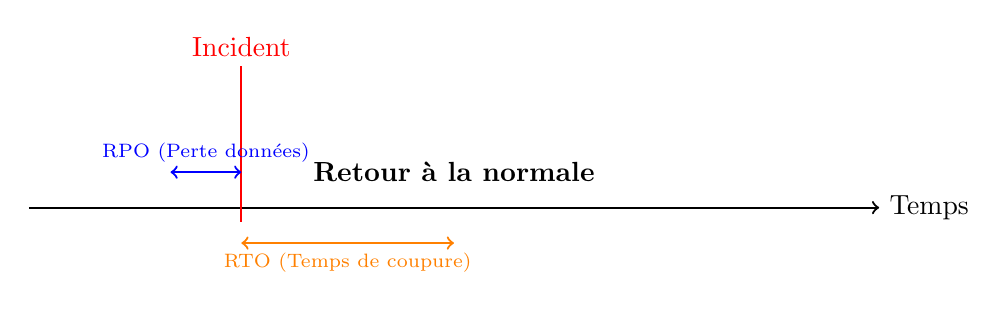
\begin{tikzpicture}[scale=0.9]
    % Axe du temps
    \draw[->, thick] (0,0) -- (12,0) node[right] {Temps};
    
    % Incident
    \draw[thick, red] (3,-0.2) -- (3,2);
    \node[above, red] at (3,2) {Incident};
    
    % RPO
    \draw[<->, thick, blue] (2,0.5) -- (3,0.5);
    \node[above, blue, font=\scriptsize] at (2.5,0.5) {RPO (Perte données)};
    
    % RTO
    \draw[<->, thick, orange] (3,-0.5) -- (6,-0.5);
    \node[below, orange, font=\scriptsize] at (4.5,-0.5) {RTO (Temps de coupure)};

    % Restauration
    \node at (6,0.5) {\textbf{Retour à la normale}};
\end{tikzpicture}
\caption{Schéma RTO vs RPO}
\end{figure}

\begin{boxlizbiz}
\textbf{Exemple LiZbiZ - Serveur ERP :}
\begin{itemize}
    \item \textbf{RTO = 4 heures :} Si l'ERP tombe, LiZbiZ doit le remettre en route en moins de 4h (sinon perturbation de la logistique).
    \item \textbf{RPO = 1 heure :} On ne peut pas perdre plus d'une heure de commandes clients.
    \textbf{Conséquence technique :} Les sauvegardes doivent être faites toutes les heures (RPO), et il faut un serveur de secours capable de démarrer rapidement (RTO).
\end{itemize}
\end{boxlizbiz}

% ------------------------------------------------------------------------------
\section{Les Stratégies de Reprise (PCA et PRA)}
% ------------------------------------------------------------------------------

\subsection{Distinction PCA / PRA}

Il ne faut pas confondre les deux plans :

\begin{itemize}
    \item \textbf{PCA (Plan de Continuité d'Activité) :} C'est le plan \textbf{Métier}. Comment l'entreprise continue de travailler si l'informatique est coupée ? (Ex: Traitement manuel des commandes, travail au papier).
    \item \textbf{PRA (Plan de Reprise d'Activité) :} C'est le plan \textbf{IT}. Comment restaurer les systèmes informatiques ? (Ex: Bascule sur un site de secours, restauration des sauvegardes).
\end{itemize}

Le PRA sert le PCA.

\subsection{Types de Sites de Secours (pour le PRA)}

Pour respecter le RTO, l'entreprise peut disposer de sites de secours :

\begin{enumerate}
    \item \textbf{Site Froid (Cold Site) :} Locaux vides, électricité et climatisation uniquement. Long à activer (semaines). Peu coûteux.
    \item \textbf{Site Tiède (Warm Site) :} Matériel présent mais éteint. Activation en jours.
    \item \textbf{Site Chaud (Hot Site) :} Matériel allumé et synchronisé en temps réel. Activation en heures (ou minutes). Très coûteux.
\end{enumerate}

% ------------------------------------------------------------------------------
\section{Cas LiZbiZ : Atelier BIA et Stratégie}
% ------------------------------------------------------------------------------

\subsection{Atelier : Définition des Besoins}

\begin{boxlizbiz}
\textbf{Scénario :} Un incendie s'est déclaré dans le local serveur principal de LiZbiZ. Toute l'infrastructure (Serveurs, ERP, Web) est détruite. Heureusement, le personnel est sain et sauf.
\end{boxlizbiz}

\textbf{Exercice de groupe :}

Pour les 3 processus suivants, définissez le RTO, le RPO et la stratégie de secours :

\begin{table}[htbp]
\centering
\small
\begin{tabular}{p{3cm}p{2cm}p{2cm}p{5cm}}
    \toprule
    \textbf{Processus} & \textbf{RTO} & \textbf{RPO} & \textbf{Stratégie Proposée} \\
    \midrule
    Site E-commerce (Vente) & 1h & 0 (Temps réel) & \textit{(A vous de jouer)} \\
    ERP (Gestion Stock) & 4h & 1h & \textit{(A vous de jouer)} \\
    Intranet RH & 1 semaine & 24h & \textit{(A vous de jouer)} \\
    \bottomrule
\end{tabular}
\end{table}

\textbf{Pistes de réflexion (Corrigé) :}
\begin{itemize}
    \item \textbf{Site Web (RTO 1h, RPO 0) :} Nécessite un Site Chaud ou une infrastructure Cloud (ex: AWS) avec réplication temps réel (Active-Active). Coût élevé mais vital pour le chiffre d'affaires.
    \item \textbf{ERP (RTO 4h, RPO 1h) :} Nécessite un Site Tiède (Warm Site) avec restauration de sauvegardes horaires. Compromis coût/performance.
    \item \textbf{Intranet RH :} Peut attendre. Site Froid ou simple restauration depuis des sauvegardes externes (tapes/Cloud froid) quand le reste est rétabli.
\end{itemize}

% ==============================================================================
% Fichier : 04_module_incident.tex (Extrait Chapitre 5)
% Description : Application Pratique - Mise en œuvre du PCA
% ==============================================================================
\chapter{Application Pratique : Mise en œuvre du PCA}
\label{chap:apppca}

La théorie de la continuité ne vaut rien sans des tests réguliers. Ce chapitre met les étudiants en situation de crise pour activer et exécuter le Plan de Continuité d'Activité (PCA) de LiZbiZ.

\section{Étape 1 : Structure du Plan (Rédaction)}
% ------------------------------------------------------------------------------

Avant de lancer la simulation, il faut structurer le document de référence.

\subsection{Composition du Document PCA}

Un PCA n'est pas un gros dossier poussiéreux. Il est composé de fiches actions immédiatement utilisables.

\begin{itemize}
    \item \textbf{Fiche de Réflexe :} Actions immédiates (Qui appeler ? Où aller ?).
    \item \textbf{Fiche de Conduite :} Procédures détaillées de basculement (PRA).
    \item \textbf{Annuaire de Crise :} Numéros de téléphone internes/externes (Délégués, Pompiers, CNIL, Assureurs).
\end{itemize}

\subsection{Organisation de la Cellule de Crise}

Le PCA définit qui prend les décisions. L'organisation type comprend :

\begin{itemize}
    \item \textbf{Cellule de Décision (Stratégique) :} PDG, DAF. Décide de la stratégie (arrêter l'activité, basculer, communiquer).
    \item \textbf{Cellule Opérationnelle (Technique) :} DSI, RSSI. Exécute le PRA (reprise informatique).
    \item \textbf{Cellule de Communication :} DRH, Marketing. Gère la communication interne et externe.
\end{itemize}

% ------------------------------------------------------------------------------
\section{Étape 2 : Simulation - Scénario "Ransomware Majeur"}
% ------------------------------------------------------------------------------

\begin{boxlizbiz}
\textbf{Scénario :}
Nous sommes le vendredi 13 à 10h00. L'attaque par Ransomware imaginée au Module 1 vient de se produire.
\begin{itemize}
    \item Tous les serveurs (ERP, Web, BDD) sont chiffrés.
    \item Les sauvegardes locales (sur le NAS du bureau) sont également chiffrées (le ransomware s'est propagé sur le réseau).
    \item Seule sauvegarde saine : Une bande magnétique externe envoyée hier soir chez un tiers-archiveur (Iron Mountain), ou une sauvegarde Cloud déconnectée.
    \item \textbf{Conséquence :} Le SI est totalement indisponible. L'entrepôt est à l'arrêt.
\end{itemize}
\end{boxlizbiz}

% ------------------------------------------------------------------------------
\section{Phase Pratique : Réaction et Bascule}
% ------------------------------------------------------------------------------

Les étudiants, répartis en groupes (Cellule de Crise), doivent accomplir les tâches suivantes.

\subsection{Mission 1 : Activation de la Cellule de Crise (15 min)}

\textbf{Livrable :} Fiche d'activation.
\begin{itemize}
    \item Qui est le Chef de Crise ? (Rôle : PDG).
    \item Qui est le Responsable Technique ? (Rôle : DSI).
    \item Rédiger un message court (SMS) pour convoquer la cellule en salle de crise.
\end{itemize}

\subsection{Mission 2 : Mise en œuvre du PRA (Technique) (45 min)}

Le groupe "Technique" doit travailler sur le rétablissement.

\textbf{Tâches :}
\begin{enumerate}
    \item \textbf{Commande de la sauvegarde :} Appeler le tiers-archiveur (simulé par un étudiant "Acteur") pour demander la restitution de la dernière bande de sauvegarde. Délai annoncé : 4 heures.
    \item \textbf{Préparation de la restauration (Lab GNS3) :}
    \begin{itemize}
        \item Accéder au serveur de backup distant (simulé) via le lab.
        \item Vérifier l'intégrité de la sauvegarde (Calcul Hash).
        \item Identifier la procédure de restauration de la Base de Données PostgreSQL.
    \end{itemize}
    \item \textbf{Estimation du RTO :} Calculer le temps total avant le retour à la normale (Temps de livraison bande + Temps de restauration + Temps de vérification). Comparer avec le RTO défini au chapitre 4.
\end{enumerate}

\subsection{Mission 3 : Mise en œuvre du PCA (Métier) (30 min)}

Le SI étant mort pour plusieurs heures, le business doit continuer (Mode Dégradé).

\textbf{Tâches :}
\begin{enumerate}
    \item \textbf{Procédure de Secours :} Proposer un processus de prise de commande manuelle pour les clients qui appellent par téléphone.
    \begin{itemize}
        \item Outils : Papier, Crayon, Terminal de paiement portable (TPE) autonome.
        \item Données : Fiche "Bon de Commande Manuel" à remplir.
    \end{itemize}
    \item \textbf{Rattrapage :} Comment réintégrer ces commandes manuelles dans l'ERP une fois le système restauré ?
\end{enumerate}

% ------------------------------------------------------------------------------
\section{Étape 3 : Communication de Crise}
% ------------------------------------------------------------------------------

\subsection{Rédaction de Communiqués}

La transparence est obligatoire.

\begin{enumerate}
    \item \textbf{Communiqué Interne :} Rassurer les salariés, dire qu'il ne faut pas utiliser l'informatique, expliquer le mode dégradé.
    \item \textbf{Communiqué Externe (Clients) :} Informer d'une panne technique, s'excuser du retard, assurer que les données sont sécurisées (ne jamais dire "Nous nous sommes fait pirater" sans validation juridique, dire "Incident technique" dans un premier temps).
\end{enumerate}

\begin{boxalert}
\textbf{Interdiction absolue :} Ne jamais communiquer sur le montant d'une rançon demandée ni sur les négociations. C'est illégal et dangereux.
\end{boxalert}

% ------------------------------------------------------------------------------
\section{Étape 4 : Retour à la Normale et RETEX}
% ------------------------------------------------------------------------------

\subsection{Clôture de la Crise}

Une fois la sauvegarde restaurée sur le Lab :
\begin{itemize}
    \item Vérifier la cohérence des données.
    \item Réouvrir l'accès aux utilisateurs progressivement.
    \item Communiquer sur la fin de l'incident.
\end{itemize}

\subsection{Le RETEX (Retour d'Expérience)}

\begin{boxlizbiz}
\textbf{Atelier final :} Organiser une réunion de debriefing (RETEX).
\begin{itemize}
    \item \textbf{Ce qui a marché :} La sauvegarde externe était saine.
    \item \textbf{Ce qui a échoué :} Le NAS local a été chiffré (Délai de restauration trop long).
    \item \textbf{Plan d'Amélioration :} Mettre en place des sauvegardes immuables (WORM - Write Once Read Many) sur le Cloud pour réduire le RTO de 8h à 2h.
\end{itemize}
\end{boxlizbiz}

% ==============================================================================
% Fichier : 04_module_incident.tex (Extrait Chapitre 6)
% Description : Evaluation du Module 3
% ==============================================================================
\chapter{Évaluation du Module 3}
\label{chap:evalmod3}

Cette évaluation valide les compétences liées à la gestion opérationnelle des incidents, l'investigation numérique (Forensics) et la planification de la continuité d'activité.

% ------------------------------------------------------------------------------
\section{Partie A : QCM (25 Questions)}
% ------------------------------------------------------------------------------

\textbf{Consigne :} Cochez la ou les bonnes réponses.

\begin{enumerate}
    \item Un événement qui compromet la sécurité de l'information est appelé :
    \begin{itemize}
        \item[A.] Un accident.
        \item[B.] Un incident.
        \item[C.] Une alerte.
        \item[D.] Un log.
    \end{itemize}

    \item La norme dédiée à la gestion des incidents de sécurité est :
    \begin{itemize}
        \item[A.] ISO 27001.
        \item[B.] ISO 27035.
        \item[C.] ISO 22301.
        \item[D.] ISO 27005.
    \end{itemize}

    \item Quel élément est le plus volatile (se perd le plus vite à l'extinction) ?
    \begin{itemize}
        \item[A.] Le disque dur.
        \item[B.] La mémoire RAM.
        \item[C.] Les sauvegardes sur bande.
        \item[D.] Les logs systèmes.
    \end{itemize}

    \item Le RTO (Recovery Time Objective) mesure :
    \begin{itemize}
        \item[A.] La quantité de données perdues.
        \item[B.] La durée cible pour rétablir le service.
        \item[C.] La fréquence des sauvegardes.
        \item[D.] Le temps de détection de l'incident.
    \end{itemize}

    \item Une "Chaîne de Custodie" (Chain of Custody) sert à :
    \begin{itemize}
        \item[A.] Verrouiller les portes du local serveur.
        \item[B.] Garantir l'intégrité et la traçabilité des preuves numériques.
        \item[C.] Connecter les serveurs entre eux.
        \item[D.] Envoyer des alertes par email.
    \end{itemize}

    \item Le RPO (Recovery Point Objective) mesure :
    \begin{itemize}
        \item[A.] Le temps de restoration.
        \item[B.] La perte de données acceptable (exprimée en temps).
        \item[C.] La distance du site de secours.
        \item[D.] Le coût de l'incident.
    \end{itemize}

    \item Un SIEM est un outil qui permet de :
    \begin{itemize}
        \item[A.] Chiffrer les disques.
        \item[B.] Centraliser les logs et corréler les événements.
        \item[C.] Gérer les mots de passe.
        \item[D.] Simuler des attaques.
    \end{itemize}

    \item La première action lors de la réaction à un incident est généralement :
    \begin{itemize}
        \item[A.] L'éradication.
        \item[B.] Le confinement.
        \item[C.] La communication.
        \item[D.] La réinstallation.
    \end{itemize}

    \item L'analyse d'impact sur l'activité (BIA) permet d'identifier :
    \begin{itemize}
        \item[A.] Les virus présents.
        \item[B.] Les fonctions vitales de l'entreprise.
        \item[C.] Les employés malveillants.
        \item[D.] Les coûts des logiciels.
    \end{itemize}

    \item Un "Faux Positif" est :
    \begin{itemize}
        \item[A.] Une alerte qui signale une menace qui n'existe pas.
        \item[B.] Un virus non détecté.
        \item[C.] Une erreur de l'administrateur.
        \item[D.] Une sauvegarde corrompue.
    \end{itemize}

    \item Le PCA (Plan de Continuité d'Activité) concerne :
    \begin{itemize}
        \item[A.] La réparation des serveurs uniquement.
        \item[B.] Le maintien des activités métier pendant la panne.
        \item[C.] La mise à jour des antivirus.
        \item[D.] Le paiement des rançons.
    \end{itemize}

    \item Un "Site Chaud" (Hot Site) est un site de secours :
    \begin{itemize}
        \item[A.] Sans matériel.
        \item[B.] Avec du matériel éteint.
        \item[C.] Avec du matériel allumé et synchronisé en temps réel.
        \item[D.] Situé dans un pays froid.
    \end{itemize}

    \item En investigation, un "Hash" sert à :
    \begin{itemize}
        \item[A.] Cacher les données.
        \item[B.] Vérifier l'intégrité d'un fichier ou d'une image disque.
        \item[C.] Accélérer le processeur.
        \item[D.] Effacer les preuves.
    \end{itemize}

    \item Le CSIRT est :
    \begin{itemize}
        \item[A.] Un logiciel de bureautique.
        \item[B.] L'équipe de réponse aux incidents de sécurité.
        \item[C.] Un type de pare-feu.
        \item[D.] Une norme juridique.
    \end{itemize}

    \item Le RETEX (Retour d'Expérience) se fait :
    \begin{itemize}
        \item[A.] Avant l'incident.
        \item[B.] Pendant l'incident.
        \item[C.] Après la résolution de l'incident.
        \item[D.] Jamais.
    \end{itemize}

    \item Un "Playbook" est :
    \begin{itemize}
        \item[A.] Un manuel de procédure de réponse à incident.
        \item[B.] Un outil de hacking.
        \item[C.] Un journal intime de l'admin.
        \item[D.] Un contrat d'assurance.
    \end{itemize}

    \item Selon le RGPD, une violation de données doit être notifiée sous :
    \begin{itemize}
        \item[A.] 24 heures.
        \item[B.] 72 heures.
        \item[C.] 1 semaine.
        \item[D.] 1 mois.
    \end{itemize}

    \item L'ordre de volatilité recommande de collecter en premier :
    \begin{itemize}
        \item[A.] Les fichiers sur le disque.
        \item[B.] Le contenu de la RAM.
        \item[C.] Les emails archivés.
        \item[D.] Les sauvegardes externes.
    \end{itemize}

    \item Le PRA (Plan de Reprise d'Activité) est :
    \begin{itemize}
        \item[A.] La version informatique du PCA.
        \item[B.] Un plan de marketing.
        \item[C.] Un plan de recrutement.
        \item[D.] Une procédure de paie.
    \end{itemize}

    \item Le "Confinement" consiste à :
    \begin{itemize}
        \item[A.] Supprimer le virus.
        \item[B.] Limiter la propagation de l'attaque.
        \item[C.] Restaurer les sauvegardes.
        \item[D.] Éteindre la lumière.
    \end{itemize}

    \item Une image disque est :
    \begin{itemize}
        \item[A.] Une photo du serveur.
        \item[B.] Une copie exacte bit-à-bit du support.
        \item[C.] Un raccourci Windows.
        \item[D.] Un fichier .jpg.
    \end{itemize}

    \item Le SOC est :
    \begin{itemize}
        \item[A.] Une équipe de surveillance 24/7.
        \item[B.] Un serveur email.
        \item[C.] Un protocole réseau.
        \item[D.] Un système d'exploitation.
    \end{itemize}

    \item La différence entre PCA et PRA est :
    \begin{itemize}
        \item[A.] PCA = Métier / PRA = Technique.
        \item[B.] PCA = Technique / PRA = Métier.
        \item[C.] Il n'y a pas de différence.
        \item[D.] PCA est pour les PME, PRA pour les grandes entreprises.
    \end{itemize}

    \item Un "Artéfact" en forensique est :
    \begin{itemize}
        \item[A.] Une pièce de musée.
        \item[B.] Une trace laissée par une activité numérique.
        \item[C.] Une erreur de code.
        \item[D.] Un objet physique.
    \end{itemize}

    \item En cas de Ransomware, la première mesure technique recommandée est souvent :
    \begin{itemize}
        \item[A.] Payer la rançon.
        \item[B.] Débrancher la machine du réseau.
        \item[C.] Redémarrer le serveur.
        \item[D.] Appeler la presse.
    \end{itemize}
\end{enumerate}

% ------------------------------------------------------------------------------
\section{Partie B : Questions Ouvertes (10 Questions)}
% ------------------------------------------------------------------------------

\textbf{Consigne :} Répondez de manière synthétique (5-10 lignes par question).

\begin{enumerate}
    \item Expliquez la différence entre un "Événement", un "Incident" et une "Crise".
    \item Pourquoi est-il déconseillé d'éteindre un serveur compromis immédiatement lors d'une investigation forensique ?
    \item Définissez le RTO et le RPO et expliquez leur relation avec le coût de la solution technique.
    \item Quelle est l'utilité d'un "Write Blocker" lors de l'acquisition d'une preuve numérique ?
    \item Expliquez le rôle du BIA dans la mise en place d'un PCA.
    \item Quelle est la différence entre un Site Froid, Tiède et Chaud ?
    \item Que signifie l'acronyme CSIRT et quel est son rôle principal ?
    \item Pourquoi le RETEX est-il une étape indispensable du cycle de vie de l'incident ?
    \item Expliquez la différence entre Correction et Éradication dans le cycle de réponse à incident.
    \item Quelles sont les informations minimales à inclure dans une fiche d'incident ?
\end{enumerate}

% ------------------------------------------------------------------------------
\section{Partie C : Cas Pratique - Mise en Condition (TP)}
% ------------------------------------------------------------------------------

\subsection{Scénario : Panne Critique du Datacenter}

\begin{boxlizbiz}
\textbf{Contexte :}
Un incendie s'est déclaré dans le local serveur principal de LiZbiZ pendant la nuit. Le système d'extinction a fonctionné, mais l'eau a endommagé l'ensemble des serveurs physiques. Le site Web est inaccessible, l'ERP est détruit. Les sauvegardes quotidiennes sont effectuées sur un Cloud externe sécurisé.
\end{boxlizbiz}

\subsection{Travaux à Réaliser (En temps limité)}

\textbf{Livrable 1 : Réaction Immédiate (30 min)}
En tant que DSI, vous coordonnez les premières heures.
\begin{itemize}
    \item Listez les 3 premières actions à réaliser (technique et humain).
    \item Définissez qui compose la Cellule de Crise (Rôles, pas de noms).
\end{itemize}

\textbf{Livrable 2 : Stratégie de Reprise (1h)}
Le PDG vous demande quand le site marchand sera de retour.
\begin{itemize}
    \item En vous basant sur le RTO défini (Chapitre 4), calculez l'impact si la restauration prend 10h.
    \item Proposez la procédure technique de restauration (PRA) depuis le Cloud.
    \item Proposez une solution de "Mode Dégradé" pour les commerciaux qui doivent répondre aux clients par téléphone.
\end{itemize}

\textbf{Livrable 3 : Rapport d'Incident (30 min)}
Rédigez la "Fiche d'Incident" finale (brève) qui servira au RETEX.
\begin{itemize}
    \item Date, Heure, Type d'incident.
    \item Cause racine (Rupture de tuyau ? Défaillance extincteur ?).
    \item Actions menées.
    \item Améliorations proposées (ex: Duplication du site).
\end{itemize}

% ==============================================================================
% Fichier : 05_module_crise.tex (Extrait Chapitre 1)
% Description : Introduction à la Gestion de Crise
% ==============================================================================

\clearpage
% ============================================================
% PARTIE IV — Gestion de Crise et RETEX
% ============================================================
\clearpage
\part{Gestion de Crise et RETEX}

\chapter{Introduction à la Gestion de Crise}
\label{chap:introcrise}

La gestion de crise est l'ultime rempart. Lorsque la prévention a échoué et que l'incident dépasse les capacités de réponse opérationnelle, l'entreprise entre en zone de turbulence. C'est un moment de vérité pour la gouvernance.

\section{Présentation : De l'Incident à la Crise}

\subsection{La Rupture de l'Équilibre}

Une panne informatique ou une attaque peut être un incident gérable. Mais elle devient une \textbf{crise} lorsqu'elle menace la pérennité de l'organisation, sa réputation, ou met en danger des vies humaines.

\begin{boxdef}
\textbf{Crise :} Événement soudain, inattendu et menaçant qui perturbe gravement le fonctionnement normal de l'organisation et nécessite des décisions rapides sous forte pression.
\end{boxdef}

La crise se caractérise souvent par :
\begin{itemize}
    \item \textbf{L'incertitude :} On ne maîtrise pas toute l'information.
    \item \textbf{L'urgence :} Le temps manque pour décider.
    \item \textbf{La pression médiatique :} L'extérieur (presse, réseaux sociaux) regarde et juge.
\end{itemize}

\subsection{Distinction Incident vs Crise}

Il est fondamental de ne pas confondre "Incident Majeur" et "Crise".

\begin{table}[htbp]
\centering
\begin{tabular}{p{4cm}p{4cm}p{4cm}}
    \toprule
    \textbf{Critère} & \textbf{Incident Majeur} & \textbf{Crise} \\
    \midrule
    \textbf{Focus} & Technique & Stratégique / Image \\
    \textbf{Gestion} & DSI / Technique & Direction Générale \\
    \textbf{Communication} & Technique (Interne) & Médiatique / Externe \\
    \textbf{Durée} & Heures à Jours & Semaines à Mois \\
    \textbf{Impact} & Arrêt activité & Survie de l'entreprise \\
    \bottomrule
\end{tabular}
\caption{Comparaison Incident Majeur et Crise}
\end{table}

\begin{boxlizbiz}
\textbf{Le "Big Bang" chez LiZbiZ :}
Jusqu'ici, le Ransomware était un incident technique (Module 3).
Ce matin, un journaliste du "Monde" appelle la direction : "Nous avons en notre possession des preuves que les données de vos clients sont en vente sur le Dark Web. Que faites-vous ?".
\textbf{Bascule :} L'incident technique devient une \textbf{Crise Médiatique et Juridique}.
\end{boxlizbiz}

% ------------------------------------------------------------------------------
\section{Concepts Clés}
% ------------------------------------------------------------------------------

\subsection{Le Seuil de Rupture}

Toute entreprise a une capacité d'absorption des chocs. La crise survient quand ce seuil est dépassé.
Ce seuil dépend de la culture de l'entreprise, de sa trésorerie, et de sa réputation préalable.

\subsection{Les Impacts Multidimensionnels}

Une crise cyber n'est jamais uniquement cyber. Elle a des répercussions en cascade :

\begin{enumerate}
    \item \textbf{Impact Financier :} Perte de CA, coût de la réparation, amendes (CNIL), baisse du cours de bourse.
    \item \textbf{Impact Réputationnel :} Perte de confiance des clients, dégradations de la marque employeur.
    \item \textbf{Impact Juridique :} Mise en cause de la responsabilité des dirigeants (infractions pénales possibles).
    \item \textbf{Impact Humain :} Stress intense, burn-out des équipes techniques, conflits internes.
\end{enumerate}

\subsection{L'Instinct de Survie}

En temps de crise, les processus habituels (comités, validations hiérarchiques longues) sont inopérants. L'entreprise doit adopter un mode de fonctionnement "commando" : centralisation de la décision et exécution rapide.

% ------------------------------------------------------------------------------
\section{Jargon de la Gestion de Crise}
% ------------------------------------------------------------------------------

\subsection{PCA vs PGC}

Il ne faut pas les confondre :

\begin{itemize}
    \item \textbf{PCA (Plan de Continuité d'Activité) :} "Comment on continue à travailler ?" (Focus : Opérations).
    \item \textbf{PGC (Plan de Gestion de Crise) :} "Comment on survit à la tempête ?" (Focus : Décision, Communication, Survie).
\end{itemize}

Le PCA est un outil technique ; le PGC est un outil de gouvernance.

\subsection{Zone de Turbulence}

Période d'intense agitation où l'information est brouillée, contradictoire et où les rumeurs fleurissent. C'est la phase la plus dangereuse.

% ------------------------------------------------------------------------------
\section{Cas LiZbiZ : Scénario "Catastrophe"}
% ------------------------------------------------------------------------------

\subsection{Mise en Situation}

\begin{boxlizbiz}
\textbf{Lundi matin, 08h30.}
Le titre boursier de LiZbiZ s'effondre de 15\% à l'ouverture.

\textbf{La cause :} Un tweet viral d'un hacker célèbre (@CyberGhost) publie un lien vers 10 000 dossiers médicaux de clients LiZbiZ (fuite de données santé).

\textbf{Réactions immédiates :}
\begin{itemize}
    \item Le standard téléphonique est saturé par les appels de clients paniqués.
    \item La boîte mail de la direction reçoit des menaces de recours collectifs.
    \item La DSI est introuvable (en réunion technique sur le Ransomware).
\end{itemize}

\textbf{Question :} Le PDG est au pied du mur. S'il ne réagit pas dans l'heure, la confiance sera définitivement perdue. C'est l'activation du PGC.
\end{boxlizbiz}

\subsection{Travaux Pratiques : Identification des Enjeux}

En groupes, les étudiants doivent lister les 3 priorités absolues pour le PDG dans les 30 prochaines minutes.

\textbf{Pistes de réflexion :}
\begin{enumerate}
    \item \textbf{Protéger les personnes :} Informer les clients concernés (Obligation RGPD).
    \item \textbf{Maîtriser l'information :} Ne pas répondre n'importe quoi aux journalistes. Préparer un "Holding Statement" (Déclaration de maintien).
    \item \textbf{Organiser le commandement :} Réunir la Cellule de Crise immédiatement.
\end{enumerate}

% ==============================================================================
% Fichier : 05_module_crise.tex (Extrait Chapitre 2)
% Description : Organisation de la Cellule de Crise
% ==============================================================================
\chapter{Organisation de la Cellule de Crise}
\label{chap:cellulecrise}

La première victime d'une crise est souvent la structure hiérarchique habituelle. Pour réagir vite, l'entreprise doit se structurer en une organisation temporaire, centralisée et souple : la Cellule de Crise.

\section{Présentation : La Structure de Commandement}
% ------------------------------------------------------------------------------

\subsection{Le Principe de Centralisation}

En temps de crise, on ne peut pas avoir plusieurs centres de décision qui se contredisent. Il faut un commandement unique. L'organisation se divise généralement en trois niveaux.

\begin{figure}[htbp]
\centering
\begin{tikzpicture}[
    node distance=1.5cm,
    box/.style={rectangle, draw, thick, fill=white, minimum width=4cm, minimum height=1cm, align=center}
]
    % Nodes
    \node[box, fill=red!20] (strat) {Cellule Stratégique\\(Direction)};
    \node[box, fill=orange!20, below left=of strat] (com) {Cellule Communication\\(Image)};
    \node[box, fill=blue!20, below right=of strat] (op) {Cellule Opérationnelle\\(Technique)};
    
    % Arrows
    \draw[->, thick] (strat) -- node[left, font=\scriptsize] {Consignes} (com);
    \draw[->, thick] (strat) -- node[right, font=\scriptsize] {Consignes} (op);
    \draw[->, thick, dashed] (op) -- node[below, font=\scriptsize] {Retours terrain} (strat);
    \draw[->, thick, dashed] (com) -- node[below, font=\scriptsize] {Retours médias} (strat);
\end{tikzpicture}
\caption{Organisation type d'une Cellule de Crise}
\end{figure}

\subsection{Les Trois Niveaux}

\begin{enumerate}
    \item \textbf{Cellule Stratégique :} Le cerveau. Elle prend les décisions majeures (Arrêter l'activité ? Payer la rançon ? Demander la mise en liquidation ?). Elle est composée de la Direction Générale.
    \item \textbf{Cellule Opérationnelle :} Les mains. Elle exécute les décisions sur le terrain (Technique, Logistique, Sécurité Physique). Elle remonte l'information factuelle.
    \item \textbf{Cellule Communication :} La voix. Elle gère l'image et la diffusion de l'information (Presse, Clients, Réseaux Sociaux).
\end{enumerate}

% ------------------------------------------------------------------------------
\section{Rôles et Responsabilités (Jargon)}
% ------------------------------------------------------------------------------

\subsection{Le Directeur de Crise}

\begin{boxdef}
\textbf{Directeur de Crise :} La personne qui anime la cellule de crise et tranche les arbitrages. Il a l'autorité ultime sur les ressources de l'entreprise pour la durée de la crise.
\end{boxdef}

C'est généralement le PDG ou le Directeur Général. Il doit être calme, décideur et protecteur de l'intérêt général de l'entreprise.

\subsection{Le Porte-parole (Spokesperson)}

\begin{boxdef}
\textbf{Porte-parole :} Seule personne habilitée à s'exprimer officiellement auprès des médias et des parties prenantes externes.
\end{boxdef}

\begin{boxalert}
\textbf{Règle d'Or :} Une seule voix ! Personne d'autre ne doit s'exprimer. Si un employé parle à la presse sans autorisation, il peut désinformé et aggraver la crise.
\end{boxalert}

\begin{boxlizbiz}
\textbf{Dilemme LiZbiZ :}
Le PDG est très charismatique mais panique facilement. La DSI est très technique mais austère.
\textbf{Choix stratégique :} Le PDG assume le rôle de Porte-parole pour rassurer (Leadership), mais il est briefé en amont par la DSI sur les faits techniques précis.
\end{boxlizbiz}

\subsection{Le Scribe (Secrétaire de Crise)}

Rôle souvent sous-estimé mais vital.

\begin{boxdef}
\textbf{Scribe :} Personne chargée de noter par écrit la chronologie des événements, les décisions prises, les actions lancées et les horaires exacts.
\end{boxdef}

Le cahier du Scribe constitue la preuve de la diligence de l'entreprise ("Nous avons réagi à 09h05"). C'est une pièce maîtresse en cas de procès futur.

\subsection{La Salle de Crise}

Lieu physique sécurisé où se réunit la cellule stratégique.
\begin{itemize}
    \item Doit être équipée (Téléphones, Projecteur, Tableaux, Alimentation électrique de secours).
    \item Doit être isolée (Confidentialité des débats).
    \item Peut être un "PC Mobile" si les locaux sont inaccessibles (ex: incendie).
\end{itemize}

% ------------------------------------------------------------------------------
\section{Cas LiZbiZ : Mise en Place de l'Organigramme}
% ------------------------------------------------------------------------------

\subsection{Scénario : Activation de la Cellule}

\begin{boxlizbiz}
\textbf{Situation :} La fuite de données est confirmée. Le PDG décide d'activer le Plan de Gestion de Crise à 09h00.
\end{boxlizbiz}

\subsection{Travaux Pratiques : Constitution des Équipes}

Les étudiants doivent répartir les rôles suivants au sein de la classe (ou en sous-groupes) :

\begin{table}[htbp]
\centering
\begin{tabular}{p{3cm}p{5cm}p{4cm}}
    \toprule
    \textbf{Rôle} & \textbf{Profil / Compétence} & \textbf{Mission Immédiate} \\
    \midrule
    Directeur de Crise & PDG (Décideur). & Arbitrer la stratégie globale. \\
    Porte-parole & Dir. Com. ou PDG. & Préparer le communiqué initial. \\
    Scribe & Juriste ou Assistant. & Noter l'heure de chaque événement. \\
    Animateur Technique & DSI / RSSI. & Faire le point sur l'étendue de la fuite. \\
    \bottomrule
\end{tabular}
\caption{Tableau de répartition des rôles LiZbiZ}
\end{table}

\subsection{Exercice : La Première Réunion}

\textbf{Consigne :} Simulez les 15 premières minutes de la réunion de crise.

\begin{enumerate}
    \item Le Directeur de Crise ouvre la séance.
    \item La DSI fait un point situation (Ce qu'on sait, ce qu'on ne sait pas).
    \item Le Scribe note : "09h05 - Confirmation fuite données santé. 09h07 - Décision d'appeler l'avocat."
    \item Débat : Faut-il prévenir la CNIL tout de suite ou attendre d'en savoir plus ? (Réponse légale : Oui, délai de 72h).
\end{enumerate}

% ==============================================================================
% Fichier : 05_module_crise.tex (Extrait Chapitre 3)
% Description : Communication de Crise
% ==============================================================================
\chapter{Communication de Crise}
\label{chap:comcrise}

En situation de crise, le temps médiatique est beaucoup plus rapide que le temps technique. Si l'entreprise ne communique pas, d'autres le feront à sa place (rumers, victimes, hackers). La communication est une arme stratégique de défense.

\section{Présentation : L'Art de la Guerre Médiatique}
% ------------------------------------------------------------------------------

\subsection{Le Temps Médiatique vs Temps Technique}

C'est le décalage le plus dangereux pour une entreprise.

\begin{itemize}
    \item \textbf{Temps Technique :} "Il nous faut 48h pour analyser les logs et comprendre l'origine de la faille." (Réalité scientifique).
    \item \textbf{Temps Médiatique :} "Twitter réclame une explication dans les 30 minutes." (Réalité émotionnelle).
\end{itemize}

Si l'entreprise attend 48h pour communiquer, la rumeur aura déjà détruit sa réputation. Il faut communiquer \textbf{avant} d'avoir toutes les réponses techniques.

\subsection{Les Objectifs de la Communication de Crise}

\begin{enumerate}
    \item \textbf{Informer :} Donner les faits connus.
    \item \textbf{Rassurer :} Montrer que l'entreprise maîtrise la situation (ou fait de son mieux).
    \item \textbf{Endiguer :} Stopper les rumeurs et les spéculations.
\end{enumerate}

% ------------------------------------------------------------------------------
\section{Concepts Clés : La Règle des 3 "T"}
% ------------------------------------------------------------------------------

La doctrine de communication de crise repose sur trois piliers :

\subsection{T comme Ténor (Porte-parole)}

Il faut une voix unique. Si le DSI dit une chose, le PDG une autre, et le commercial une troisième, l'entreprise perd toute crédibilité.

\begin{boxalert}
\textbf{Erreur fréquente :} Laisser un expert technique (DSI) s'exprimer avec un jargon incompréhensible ("On a eu une injection SQL sur le port 80..."). Le public entend : "On ne sait pas ce qui se passe".
\end{boxalert}

\subsection{T comme Transparence}

Il ne faut pas mentir. Un mensonge découvert est pire que la crise elle-même. On peut dire "Nous ne savons pas encore", mais on ne doit pas dire "Tout va bien" si ce n'est pas vrai.

\subsection{T comme Temporalité}

Il faut communiquer vite et régulièrement.
\begin{itemize}
    \item \textbf{Holding Statement :} Déclaration initiale très courte (souvent dans l'heure). "Nous avons détecté un incident, nos équipes sont mobilisées."
    \item \textbf{Points de situation (SitRep) :} Mises à jour régulières (ex: toutes les 4 heures) même s'il n'y a rien de nouveau. Cela montre que l'entreprise est active.
\end{itemize}

% ------------------------------------------------------------------------------
\section{Les Cibles de Communication}
% ------------------------------------------------------------------------------

On ne parle pas de la même façon à tout le monde.

\begin{table}[htbp]
\centering
\begin{tabular}{p{3cm}p{4cm}p{5cm}}
    \toprule
    \textbf{Cible} & \textbf{Objectif} & \textbf{Message Type} \\
    \midrule
    \textbf{Interne (Salariés)} & Maintenir le lien, éviter la panique. "On ne parle pas à la presse." & "Voici la situation, voici ce qu'il faut faire (ne rien dire), nous vous tiendrons au courant." \\
    \textbf{Clients / Victimes} & Dédommagement, empathie, fidélité. & "Nous sommes désolés, voici les mesures de protection que nous mettons en place pour vous." \\
    \textbf{Médias / Public} & Préserver l'image, corriger les faits. & "L'incident est maîtrisé. L'entreprise est résiliente." \\
    \textbf{Autorités (CNIL)} & Conformité légale. & "Notification de violation de données selon l'article 33 RGPD." \\
    \bottomrule
\end{tabular}
\caption{Matrice des cibles de communication}
\end{table}

% ------------------------------------------------------------------------------
\section{Les Interdits (Les "Tues")}
% ------------------------------------------------------------------------------

Il y a des choses qu'il ne faut jamais faire en communication de crise :

\begin{enumerate}
    \item \textbf{Minimiser :} "Ce n'est qu'une petite fuite". (Manque de respect pour les victimes).
    \item \textbf{Démentir sans preuve :} "Nos systèmes sont infaillibles". (Démenti souvent contredit par la suite).
    \item \textbf{Culpabiliser la victime :} "Si le client avait utilisé un mot de passe fort...". (Inadmissible).
    \item \textbf{Parler de rançon :} Ne jamais communiquer sur le montant ou le fait de payer une rançon (illégal / dangereux).
\end{enumerate}

% ------------------------------------------------------------------------------
\section{Cas LiZbiZ : Atelier d'Écriture}
% ------------------------------------------------------------------------------

\subsection{Scénario : La Vague de Panique}

\begin{boxlizbiz}
\textbf{10h00 :} L'article du "Monde" est paru. Le titre : "LiZbiZ met en danger vos données de santé".
Le standard explose. Les clients suppriment leurs comptes. Il faut réagir \textbf{maintenant}.
\end{boxlizbiz}

\subsection{Mission : Rédiger le "Holding Statement"}

Les étudiants doivent rédiger un communiqué de 10 lignes maximum pour être posté sur le site web de LiZbiZ et envoyé à la presse. Il doit respecter la structure :

\begin{enumerate}
    \item \textbf{Les Faits :} Reconnaître l'incident (sans donner de détails techniques sensibles).
    \item \textbf{L'Action :} Dire ce qui est fait (mobilisation des experts, notification CNIL).
    \item \textbf{L'Empathie :} S'excuser sincèrement.
    \item \textbf{Le Suivi :} Donner un canal d'information dédié.
\end{enumerate}

\textbf{Exemple de mauvais communiqué (à éviter) :}
\textit{"Suite à une attaque complexe de hackers sophistiqués que personne n'aurait pu prévoir, certains documents ont pu être consultés. Nos équipes informatiques travaillent dur. Nous vous tiendrons au courant."} (Passif, technique, manque d'empathie).

\textbf{Exemple de bon communiqué (à reproduire) :}
\textit{"LiZbiZ confirme avoir été victime d'une cyberattaque affectant la confidentialité de certaines données clients. Nous sommes profondément désolés pour ce préjudice. La sécurité de vos données est notre priorité absolue. Nous avons immédiatement mobilisé nos experts et notifié la CNIL. Une cellule d'écoute est activée au 0800XXXXXX pour répondre à vos questions. Nous vous tiendrons informés toutes les 4 heures."} (Actif, empathique, concret).

% ==============================================================================
% Fichier : 05_module_crise.tex (Extrait Chapitre 4)
% Description : La Simulation de Crise (Exercice Tabletop)
% ==============================================================================
\chapter{La Simulation de Crise (Exercice Tabletop)}
\label{chap:simcrise}

La théorie est utile, mais la gestion de crise s'apprend par la pratique. Ce chapitre est dédié à un exercice de simulation de type \textbf{Tabletop} (exercice sur table). Il ne s'agit pas de tests techniques informatiques, mais de mise en situation des processus de décision et de communication.

\section{Présentation de l'Exercice}
% ------------------------------------------------------------------------------

\subsection{Objectifs Pédagogiques}

\begin{itemize}
    \item Tester la montée en puissance de la Cellule de Crise.
    \item Exercer la prise de décision sous pression et avec une information incomplète.
    \item Pratiquer la coordination entre les cellules (Stratégique, Opérationnel, Communication).
    \item Identifier les failles du Plan de Gestion de Crise (PGC).
\end{itemize}

\subsection{Mécanique du Jeu (Time Compression)}

L'exercice se déroule sur 1h30 en classe, mais simule une journée de crise (24h).
Le formateur joue le rôle du "Maître du Jeu" (Game Master) et injecte des événements (Twists) qui changent la donne.

% ------------------------------------------------------------------------------
\section{Phase 0 : Briefing et Attribution des Rôles (15 min)}
% ------------------------------------------------------------------------------

\subsection{Distribution des Rôles}

Les étudiants sont répartis en sous-groupes ou jouent individuellement les rôles clés définis au Chapitre 2.

\begin{table}[htbp]
\centering
\begin{tabular}{p{4cm}p{8cm}}
    \toprule
    \textbf{Rôle (Étudiant)} & \textbf{Objectif Personnel} \\
    \midrule
    \textbf{PDG (Directeur de Crise)} & Préserver l'entreprise, trancher les arbitrages difficiles. \\
    \textbf{DSI (Resp. Opérationnel)} & Restaurer le SI, fournir des faits techniques fiables. \\
    \textbf{Dir. Com (Porte-parole)} & Protéger l'image, rédiger les communiqués. \\
    \textbf{Juriste (DPO)} & Assurer la conformité (RGPD), protéger les dirigeants pénalement. \\
    \textbf{DRH} & Gérer le stress interne, empêcher les fuites salariés. \\
    \textbf{Scribe} & Noter la timeline exacte. \\
    \bottomrule
\end{tabular}
\caption{Matrice des rôles pour le Tabletop}
\end{table}

\subsection{Contexte Initial}

Le Maître du Jeu lit l'introduction :
\begin{quote}
"Nous sommes vendredi 17h00. LiZbiZ s'apprête à fermer pour le week-end. Soudain, le téléphone du DSI sonne : tous les écrans de l'entrepôt affichent un message rouge 'Your files are encrypted'. Le téléphone du standard commence à sonner : un client tweet qu'il a reçu un email de rançon avec ses données personnelles en pièce jointe."
\end{quote}

% ------------------------------------------------------------------------------
\section{Phase 1 : La Réaction Immédiate (20 min)}
% ------------------------------------------------------------------------------

\textbf{Temps simulé :} Vendredi 17h15.

\subsection{Consignes pour les équipes}
\begin{itemize}
    \item \textbf{Stratégie :} Décidez-vous d'éteindre les serveurs ? Prévenez-vous la police ?
    \item \textbf{Communication :} Que dites-vous aux employés qui rentrent chez eux ?
    \item \textbf{Opérationnel :} Quels sont les premiers diagnostics ?
\end{itemize}

\subsection{Injection d'Événement (Twist 1)}
Le Maître du Jeu annonce :
\begin{quote}
"Un journaliste du 'Figaro' appelle le standard. Il a connaissance de la rançon et demande si LiZbiZ a l'intention de payer. La réponse est attendue dans 10 minutes."
\end{quote}

% ------------------------------------------------------------------------------
\section{Phase 2 : L'Escalade (20 min)}
% ------------------------------------------------------------------------------

\textbf{Temps simulé :} Vendredi 20h00.

\subsection{Injection d'Événement (Twist 2)}
\begin{quote}
"La CNIL appelle la direction. Ils ont été alertés par un collectif de défense des consommateurs. Ils demandent le rapport de violation complet pour lundi matin."
\end{quote}

\subsection{Consignes pour les équipes}
\begin{itemize}
    \item \textbf{Juridique :} Que répondez-vous à la CNIL ? Avez-vous toutes les infos requises (Article 33 RGPD) ?
    \item \textbf{Technique :} L'attaquant a-t-il accédé les données de santé (risque élevé) ou juste les noms ?
\end{itemize}

% ------------------------------------------------------------------------------
\section{Phase 3 : La Tempête Médiatique (20 min)}
% ------------------------------------------------------------------------------

\textbf{Temps simulé :} Samedi 10h00.

\subsection{Injection d'Événement (Twist 3)}
\begin{quote}
"Le hashtag \#LiZbiZDataLeak est en tendance sur Twitter (X). Une fausse rumeur circule : 'La banque de LiZbiZ a fait faillite, tout l'argent est bloqué'. Les clients paniquent et demandent des remboursements massifs."
\end{quote}

\subsection{Consignes pour les équipes}
\begin{itemize}
    \item \textbf{Communication :} Organisez une conférence de presse simulée (Questions/Réponses avec le reste de la classe jouant les journalistes).
    \item \textbf{Stratégie :} Démentez-vous la rumeur bancaire ? Comment séparer le problème cyber du problème financier ?
\end{itemize}

% ------------------------------------------------------------------------------
\section{Phase 4 : Résolution et Debriefing (15 min)}
% ------------------------------------------------------------------------------

\textbf{Temps simulé :} Lundi 09h00. L'ERP est restauré à partir des sauvegardes saines.

\subsection{Fin de l'Exercice}

Le Maître du Jeu arrête le chronomètre. L'exercice s'arrête.

\subsection{Le "Hotwash" (RETEX à chaud)}

C'est le moment le plus important de l'apprentissage. On passe en revue ce qui s'est passé.

\textbf{Questions de debriefing :}
\begin{enumerate}
    \item \textbf{Decision Making :} Les décisions ont-elles été prises rapidement ? Manquait-on d'informations ?
    \item \textbf{Communication :} Le message a-t-il été cohérent ? A-t-on dit des choses contradictoires ?
    \item \textbf{Rôles :} Le PDG a-t-il été débordé par la technique ? Le DSI a-t-il été trop long à diagnostiquer ?
    \item \textbf{Leçons :} Qu'est-ce qu'on ferait différemment la prochaine fois ?
\end{enumerate}

\begin{boxalert}
\textbf{Conclusion typique :} On réalise souvent que la Cellule de Crise a passé trop de temps à chercher des informations techniques précises (Qui ? Comment ?) et pas assez à gérer l'émotion des clients et des employés. La leçon : En crise, l'humain et la communication priment sur la technique pure.
\end{boxalert}

% ==============================================================================
% Fichier : 05_module_crise.tex (Extrait Chapitre 5)
% Description : Le Retour d'Expérience (RETEX)
% ==============================================================================
\chapter{Le Retour d'Expérience (RETEX)}
\label{chap:retex}

La crise est terminée, le système est restauré et la communication s'est apaisée. Pourtant, le travail n'est pas fini. La dernière étape, souvent négligée par fatigue, est la plus importante pour l'avenir : le Retour d'Expérience (RETEX). C'est l'essence même de l'amélioration continue.

\section{Présentation : Boucler la Boucle PDCA}
% ------------------------------------------------------------------------------

\subsection{Définition}

\begin{boxdef}
\textbf{RETEX (Retour d'Expérience) :} Processus structuré visant à analyser un événement passé pour en tirer des enseignements (leçons) et mettre en œuvre des actions correctives afin d'améliorer la sécurité et la résilience de l'organisation.
\end{boxdef}

Sans RETEX, l'entreprise est condamnée à revivre la même crise de la même manière. C'est le moment où l'on transforme l'échec en capital d'expérience.

\subsection{Le but : Passer de l'Identifié à l'Appris}

Il existe une différence majeure entre une leçon identifiée et une leçon apprise.
\begin{itemize}
    \item \textbf{Leçon Identifiée :} "Nous avons vu que le plan de sauvegarde n'était pas testé." (Constat).
    \item \textbf{Leçon Apprise :} "Nous avons mis en place des tests de sauvegarde mensuels obligatoires." (Action).
\end{itemize}

Le RETEX n'est valide que s'il débouche sur des actions concrètes.

% ------------------------------------------------------------------------------
\section{Les Deux Phases du RETEX}
% ------------------------------------------------------------------------------

\subsection{RETEX à Chaud (Hotwash)}

\begin{boxdef}
\textbf{RETEX à Chaud :} Réunion de debriefing organisée très rapidement après la fin de la crise (J+1 à J+3), alors que les souvenirs sont frais.
\end{boxdef}

\textbf{Objectifs :}
\begin{itemize}
    \item Recueillir les faits et les ressenti immédiats.
    \item Féliciter les équipes (reconnaissance du travail fourni).
    \item Identifier les problèmes bloquants évidents.
    \item Clore symboliquement la période de crise pour le personnel.
\end{itemize}

C'est souvent une réunion "débriefing" sans prise de notes formelle excessive, mais avec un compte-rendu rapide.

\subsection{RETEX à Froid (Coldwash)}

\begin{boxdef}
\textbf{RETEX à Froid :} Analyse approfondie réalisée plusieurs semaines après la crise (J+30 à J+60), avec du recul et l'accès à toutes les données techniques (logs, rapports d'audit).
\end{boxdef}

\textbf{Objectifs :}
\begin{itemize}
    \item Analyser les causes racines (Pourquoi ça a commencé ?).
    \item Analyser la gestion de la crise (Pourquoi a-t-on réagi comme ça ?).
    \item Mettre à jour les documents (PCA, PRA, Plans de crise).
    \item Définir le plan d'investissement futur.
\end{itemize}

% ------------------------------------------------------------------------------
\section{Outils d'Analyse : Comprendre le "Pourquoi"}
% ------------------------------------------------------------------------------

Pour éviter que l'incident ne se reproduise, il faut chercher la \textbf{Cause Racine} (Root Cause), et pas seulement la cause immédiate.

\subsection{La Chronologie (Timeline)}

Reconstituer la frise chronologique précise :
\begin{itemize}
    \item Heure de l'intrusion.
    \item Heure de la détection.
    \item Heure de la prise de conscience.
    \item Heure de la communication.
\end{itemize}

L'écart entre l'intrusion et la détection est souvent le point critique à améliorer.

\subsection{La méthode des "5 Pourquois" (5 Whys)}

Technique simple pour descendre en profondeur.

\begin{boxlizbiz}
\textbf{Exemple LiZbiZ :}
\begin{enumerate}
    \item \textbf{Pourquoi} l'ERP a-t-il été chiffré ? \textit{Car le Ransomware s'est propagé.}
    \item \textbf{Pourquoi} s'est-il propagé ? \textit{Car le VLAN IoT n'était pas isolé.}
    \item \textbf{Pourquoi} n'était-il pas isolé ? \textit{Car la règle firewall était en "Allow All".}
    \item \textbf{Pourquoi} "Allow All" ? \textit{Car un technicien avait ouvert le flux pour un test et a oublié de le refermer.}
    \item \textbf{Pourquoi} a-t-il oublié ? \textit{Car il n'y a pas de procédure de validation des règles firewall (Cause Racine).}
\end{enumerate}
\textbf{Action :} Mettre en place une revue mensuelle des règles firewall.
\end{boxlizbiz}

\subsection{Le Diagramme d'Ishikawa (Causes et Effets)}

Outil visuel pour classer les causes par familles (5M : Méthodes, Main d'œuvre, Matériel, Milieu, Matière).

% ------------------------------------------------------------------------------
\section{Cas LiZbiZ : Le Rapport Final}
% ------------------------------------------------------------------------------

\subsection{Mission : Rédiger le Rapport RETEX}

\begin{boxlizbiz}
\textbf{Contexte :} Un mois après la crise du Ransomware et de la fuite de données. L'entreprise tourne à nouveau normalement. Vous êtes chargé par le COMEX de produire le rapport de synthèse.
\end{boxlizbiz}

\textbf{Structure du rapport à produire (Travail de synthèse) :}

\begin{enumerate}
    \item \textbf{Résumé de l'incident :} Faits majeurs et impacts financiers/image.
    \item \textbf{Analyse des Causes Racines :} Résultat de l'enquête technique (Logs, Forensics).
    \item \textbf{Bilan de la Réponse :}
    \begin{itemize}
        \item \textbf{Points Forts :} Ce qui a fonctionné (ex: Synchronisation des sauvegardes externes, mobilisation des équipes).
        \item \textbf{Points Faibles :} Ce qui a échoué (ex: Temps de détection trop long, confusion dans la communication interne, absence de plan spécifique Ransomware).
    \end{itemize}
    \item \textbf{Plan d'Amélioration :}
    \begin{itemize}
        \item \textbf{Court terme (1 mois) :} Isoler les réseaux, changer les mots de passe.
        \item \textbf{Moyen terme (6 mois) :} Déployer un EDR (Endpoint Detection and Response), former le CSIRT.
        \item \textbf{Long terme (1 an) :} Obtenir la certification ISO 27001.
    \end{itemize}
\end{enumerate}

\subsection{Clôture du Cours}

Ce rapport RETEX finalise le cycle de vie de la sécurité vu dans ce cours :
\begin{center}
\textbf{Gouvernance $\rightarrow$ Risque $\rightarrow$ Audit $\rightarrow$ Incident $\rightarrow$ Crise $\rightarrow$ RETEX $\rightarrow$ Gouvernance (Améliorée)}
\end{center}

% ==============================================================================
% Fichier : 05_module_crise.tex (Extrait Chapitre 6)
% Description : Evaluation du Module 4
% ==============================================================================
\chapter{Évaluation du Module 4}
\label{chap:evalmod4}

Cette évaluation finale valide les compétences liées à la gestion stratégique de la crise, la communication sous pression et l'analyse post-incident (RETEX).

% ------------------------------------------------------------------------------
\section{Partie A : QCM (25 Questions)}
% ------------------------------------------------------------------------------

\textbf{Consigne :} Cochez la ou les bonnes réponses.

\begin{enumerate}
    \item Une crise se caractérise principalement par :
    \begin{itemize}
        \item[A.] Une panne technique prolongée.
        \item[B.] Une menace pour la survie ou la réputation de l'entreprise.
        \item[C.] Un besoin de communication externe.
        \item[D.] Un incident mineur.
    \end{itemize}

    \item Le PGC (Plan de Gestion de Crise) est un outil :
    \begin{itemize}
        \item[A.] Technique (informatique).
        \item[B.] Stratégique (organisationnel et humain).
        \item[C.] Financier.
        \item[D.] Commercial.
    \end{itemize}

    \item Le "Holding Statement" est :
    \begin{itemize}
        \item[A.] Un communiqué détaillé post-crise.
        \item[B.] Une déclaration initiale courte pour occuper le terrain médiatique.
        \item[C.] Un rapport technique.
        \item[D.] Une promesse de dédommagement.
    \end{itemize}

    \item La règle des "3 T" en communication de crise signifie :
    \begin{itemize}
        \item[A.] Technique, Travail, Temps.
        \item[B.] Ténor, Transparence, Temporalité.
        \item[C.] Test, Tolérance, Terme.
        \item[D.] Twitter, TikTok, Telegram.
    \end{itemize}

    \item Le rôle du "Scribe" dans une cellule de crise est de :
    \begin{itemize}
        \item[A.] Rédiger les communiqués de presse.
        \item[B.] Noter la chronologie des faits et décisions.
        \item[C.] Réparer les serveurs.
        \item[D.] Répondre au téléphone.
    \end{itemize}

    \item Le RETEX à chaud (Hotwash) se déroule :
    \begin{itemize}
        \item[A.] Avant la crise.
        \item[B.] Juste après la fin de la crise.
        \item[C.] Un an après.
        \item[D.] Pendant la simulation.
    \end{itemize}

    \item Le "Porte-parole" est la personne chargée de :
    \begin{itemize}
        \item[A.] Gérer les budgets.
        \item[B.] S'exprimer officiellement auprès des médias.
        \item[C.] Analyser les logs techniques.
        \item[D.] Déléguer les tâches techniques.
    \end{itemize}

    \item La méthode des "5 Pourquois" sert à :
    \begin{itemize}
        \item[A.] Trouver la cause racine d'un problème.
        \item[B.] Préparer un communiqué.
        \item[C.] Calculer le coût d'une crise.
        \item[D.] Définir le RTO.
    \end{itemize}

    \item Une crise est souvent déclenchée par le "Big Bang informationnel", qui est :
    \begin{itemize}
        \item[A.] L'explosion du serveur.
        \item[B.] Le moment où l'information devient publique.
        \item[C.] La fin de la crise.
        \item[D.] La détection technique.
    \end{itemize}

    \item Il est interdit en communication de crise de :
    \begin{itemize}
        \item[A.] Dire qu'on ne sait pas.
        \item[B.] Minimiser les faits ou mentir.
        \item[C.] Montrer de l'empathie.
        \item[D.] Déléguer la parole.
    \end{itemize}

    \item La Cellule de Crise doit être :
    \begin{itemize}
        \item[A.] Grande (plus de 20 personnes).
        \item[B.] Restreinte et décisionnaire.
        \item[C.] Composée uniquement de techniciens.
        \item[D.] Composée uniquement de juristes.
    \end{itemize}

    \item Le temps médiatique est généralement :
    \begin{itemize}
        \item[A.] Plus lent que le temps technique.
        \item[B.] Plus rapide que le temps technique.
        \item[C.] Égal au temps technique.
        \item[D.] Sans importance.
    \end{itemize}

    \item Un exercice "Tabletop" est :
    \begin{itemize}
        \item[A.] Un test de restauration de sauvegarde.
        \item[B.] Une simulation de gestion de crise autour d'une table.
        \item[C.] Un audit de sécurité.
        \item[D.] Une réunion mensuelle.
    \end{itemize}

    \item En cas de fuite de données, l'entreprise doit notifier la CNIL sous :
    \begin{itemize}
        \item[A.] 72 heures.
        \item[B.] 24 heures.
        \item[C.] 1 semaine.
        \item[D.] Il n'y a pas d'obligation.
    \end{itemize}

    \item La cause racine est :
    \begin{itemize}
        \item[A.] La dernière personne à avoir touché le serveur.
        \item[B.] La raison fondamentale qui a permis l'incident.
        \item[C.] Le symptôme visible.
        \item[D.] La conséquence financière.
    \end{itemize}

    \item Le Directeur de Crise est généralement :
    \begin{itemize}
        \item[A.] Le DSI.
        \item[B.] Le PDG ou un membre du COMEX.
        \item[C.] Le RSSI.
        \item[D.] Le stagiaire.
    \end{itemize}

    \item Une "Leçon Apprise" implique :
    \begin{itemize}
        \item[A.] D'avoir identifié le problème.
        \item[B.] D'avoir mis en place une action corrective effective.
        \item[C.] D'avoir lu le rapport.
        \item[D.] D'avoir oublié l'incident.
    \end{itemize}

    \item Face aux médias, l'attitude recommandée est :
    \begin{itemize}
        \item[A.] "No comment" (Aucun commentaire).
        \item[B.] Fuite ou agressivité.
        \item[C.] Maîtrise et empathie.
        \item[D.] Jargon technique.
    \end{itemize}

    \item La "Zone de Turbulence" est :
    \begin{itemize}
        \item[A.] La période où l'information est confuse et les rumeurs fortes.
        \item[B.] Le local serveur.
        \item[C.] Le site de secours.
        \item[D.] La phase de test.
    \end{itemize}

    \item Le RETEX permet :
    \begin{itemize}
        \item[A.] De chercher des coupables.
        \item[B.] D'améliorer le système pour l'avenir.
        \item[C.] D'archiver les logs.
        \item[D.] De licencier des employés.
    \end{itemize}

    \item La communication interne en temps de crise doit viser à :
    \begin{itemize}
        \item[A.] Cacher la vérité aux employés.
        \item[B.] Mobiliser et rassurer le personnel.
        \item[C.] Demander aux employés de parler à la presse.
        \item[D.] Annuler les congés sans explication.
    \end{itemize}

    \item Un "Twist" dans une simulation est :
    \begin{itemize}
        \item[A.] Un événement inattendu qui change la donne.
        \item[B.] Une danse de victoire.
        \item[C.] Une sauvegarde réussie.
        \item[D.] Un type de ransomware.
    \end{itemize}

    \item Le seuil de rupture est :
    \begin{itemize}
        \item[A.] Le moment où l'entreprise ne peut plus absorber le choc seule.
        \item[B.] La limite de stockage du disque.
        \item[C.] La fin de la journée de travail.
        \item[D.] Le seuil de rentabilité.
    \end{itemize}

    \item Le diagramme d'Ishikawa classe les causes en :
    \begin{itemize}
        \item[A.] 5M (Méthodes, Main d'œuvre, Matériel, Milieu, Matière).
        \item[B.] 5T (Temps, Travail, Technique...).
        \item[C.] 3C (Coût, Crise, Communication).
        \item[D.] A, B, C, D.
    \end{itemize}

    \item Après une crise, le document final qui synthétise tout est :
    \begin{itemize}
        \item[A.] La facture.
        \item[B.] Le rapport RETEX.
        \item[C.] Le PRA.
        \item[D.] L'email de licenciement.
    \end{itemize}
\end{enumerate}

% ------------------------------------------------------------------------------
\section{Partie B : Questions Ouvertes (10 Questions)}
% ------------------------------------------------------------------------------

\textbf{Consigne :} Répondez de manière synthétique (5-10 lignes par question).

\begin{enumerate}
    \item Expliquez la différence fondamentale entre un incident majeur et une crise.
    \item Pourquoi le rôle du Scribe est-il si important pour la protection juridique de l'entreprise ?
    \item Quels sont les risques à laisser un technicien (DSI) jouer le rôle de porte-parole face aux médias ?
    \item Définissez la règle des 3 T en communication de crise.
    \item Quelle est la différence entre le RETEX à chaud et le RETEX à froid ?
    \item Expliquez le concept de "Cause Racine" et son importance pour éviter la récidive.
    \item Pourquoi est-il dangereux de dire "No comment" face à la presse ?
    \item Quelles sont les trois cellules principales d'une organisation de crise et leurs rôles respectifs ?
    \item Comment la méthode des 5 Pourquois aide-t-elle à dépasser les symptômes visibles d'un problème ?
    \item Pourquoi le cycle PDCA est-il la philosophie sous-jacente du RETEX ?
\end{enumerate}

% ------------------------------------------------------------------------------
\section{Partie C : Cas Pratique - Synthèse Finale}
% ------------------------------------------------------------------------------

\subsection{Scénario : L'Après-Crise de LiZbiZ}

\begin{boxlizbiz}
\textbf{Contexte :}
La crise du Ransomware et de la fuite de données est terminée depuis deux semaines. Le PDG de LiZbiZ vous demande de clore le dossier. L'entreprise a subi une perte de chiffre d'affaires de 15\% et une amende de la CNIL, mais a survécu.
\end{boxlizbiz}

\subsection{Travaux à Réaliser (Projet de fin de cours)}

\textbf{Livrable 1 : Rapport RETEX Court (1h)}
Rédigez un document synthétique incluant :
\begin{enumerate}
    \item \textbf{Timeline :} Résumez la séquence (Détection $\rightarrow$ Crise $\rightarrow$ Résolution).
    \item \textbf{5 Pourquois :} Appliquez la méthode sur le fait que "La sauvegarde locale a été chiffrée". (Pourquoi était-elle locale ? Pourquoi connectée ? etc.).
    \item \textbf{Leçons Apprises :} Identifiez 2 points forts et 2 points faibles de la gestion de crise par LiZbiZ.
\end{enumerate}

\textbf{Livrable 2 : Plan d'Amélioration (30 min)}
Proposez 3 actions concrètes (Technique, Organisationnel, Humain) pour que cet incident ne se reproduise jamais.

\textbf{Livrable 3 : Communication de Clôture (30 min)}
Rédigez un email interne à destination de tous les salariés de LiZbiZ pour tourner la page, remercier les équipes et présenter les mesures prises pour l'avenir.

% ==============================================================================
% Fichier : 06_resume.tex
% Description : Résumé et points clés du cours
% ==============================================================================

% --- Résumé et Évaluation Finale ---
\chapter{Résumé du Cours : L'Essentiel à Retenir}
\label{chap:resume}

Ce chapitre synthétise les concepts fondamentaux abordés dans les quatre modules du cours. Il sert de mémo pour les professionnels et de guide de révision pour les examens.

\section{Module 1 : Gouvernance et Analyse de Risque}
\textbf{Concept clé :} Le risque est le produit de la Probabilité par la Gravité. On ne peut pas éliminer tous les risques, on doit les gérer (Accepter, Réduire, Éviter, Transférer).
\begin{itemize}
    \item \textbf{ISO 27005 / EBIOS RM :} Méthodes pour identifier et traiter les risques.
    \item \textbf{RACI :} Outil indispensable pour définir qui fait, qui décide, qui consulte, qui informe.
    \item \textbf{RSSI :} Responsable ultime de la sécurité (Accountable), mais pas seul acteur.
\end{itemize}

\section{Module 2 : Audit et Management de la Qualité}
\textbf{Concept clé :} L'audit mesure l'écart entre ce qui est prévu (référentiel) et ce qui est fait (réalité). Il nécessite indépendance et preuves.
\begin{itemize}
    \item \textbf{ISO 19011 :} La norme "méthode" pour conduire un audit.
    \item \textbf{ISO 27001 :} La norme "exigence" pour le SMSI (certification).
    \item \textbf{Non-Conformité :} Écart constaté. Distinction Majeure (systémique) vs Mineure (isolée).
    \item \textbf{PAC :} Plan d'Actions Correctives (Correction immédiate + Action de fond).
\end{itemize}

\section{Module 3 : Gestion des Incidents et Continuité}
\textbf{Concept clé :} L'incident est inévitable. La résilience se mesure à la capacité de reprise (RTO/RPO).
\begin{itemize}
    \item \textbf{ISO 27035 :} Cycle de vie de l'incident (Détection, Confinement, Éradication, Rétablissement).
    \item \textbf{Forensics :} Investigation numérique. Règle d'or : ne rien altérer (Ordre de volatilité : RAM d'abord).
    \item \textbf{BIA (Business Impact Analysis) :} Analyse pour identifier les fonctions vitales.
    \item \textbf{RTO/RPO :} Objectifs de Temps de Reprise et Perte de Données acceptable.
    \item \textbf{PCA/PRA :} Plan de Continuité (Métier) vs Plan de Reprise (IT).
\end{itemize}

\section{Module 4 : Gestion de Crise et Retex}
\textbf{Concept clé :} La crise est un incident qui menace la survie de l'entreprise. Elle demande une gestion humaine et médiatique, pas seulement technique.
\begin{itemize}
    \item \textbf{Cellule de Crise :} Structure temporaire centralisée (Stratégique, Opérationnel, Communication).
    \item \textbf{Règle des 3 T :} Ténor (Porte-parole unique), Transparence, Temporalité (vitesse).
    \item \textbf{RETEX :} Retour d'expérience. Indispensable pour l'amélioration continue (PDCA). Distinction à chaud (immédiat) et à froid (analyse profonde).
\end{itemize}

% ==============================================================================
% Fichier : 07_evaluation_finale.tex
% Description : Evaluation Finale Globale
% ==============================================================================
\chapter{Évaluation Finale Globale}
\label{chap:evalfinale}

Cette évaluation couvre l'intégralité du programme : Gouvernance, Risque, Audit, Incident, Continuité et Crise.

% ------------------------------------------------------------------------------
% PARTIE A : QCM (Selection représentative)
% ------------------------------------------------------------------------------
\section{Partie A : QCM (Choisir la bonne réponse)}

\subsection*{Module 1 : Gouvernance et Risque}
\begin{enumerate}
    \item Le "Accountable" dans une matrice RACI est :
    \begin{itemize} \item[A.] Celui qui fait le travail. \item[B.] Celui qui rend des comptes. \item[C.] Celui qu'on informe. \end{itemize}
    \item La méthode d'analyse de risque française est :
    \begin{itemize} \item[A.] NIST. \item[B.] EBIOS RM. \item[C.] OCTAVE. \end{itemize}
    \item La criticité se calcule par :
    \begin{itemize} \item[A.] Probabilité + Gravité. \item[B.] Probabilité $\times$ Gravité. \item[C.] Coût $\times$ Temps. \end{itemize}
    \item Une vulnérabilité est :
    \begin{itemize} \item[A.] Une faiblesse. \item[B.] Un pirate. \item[C.] Un impact. \end{itemize}
    \item Souscrire une assurance cyber est une stratégie de :
    \begin{itemize} \item[A.] Réduction. \item[B.] Acceptation. \item[C.] Transfert. \end{itemize}
    \item Le RSSI reporte généralement à :
    \begin{itemize} \item[A.] La DSI. \item[B.] La Direction Générale. \item[C.] Le Service RH. \end{itemize}
    \item Le risque résiduel est :
    \begin{itemize} \item[A.] Le risque avant traitement. \item[B.] Le risque après traitement. \item[C.] Un risque imaginaire. \end{itemize}
    \item L'ISO 31000 concerne :
    \begin{itemize} \item[A.] La qualité. \item[B.] Le management du risque. \item[C.] L'audit. \end{itemize}
    \item L'appétence au risque est définie par :
    \begin{itemize} \item[A.] Le RSSI. \item[B.] La Direction (COMEX). \item[C.] L'auditeur. \end{itemize}
    \item Un actif essentiel est :
    \begin{itemize} \item[A.] Un serveur. \item[B.] Un processus métier critique. \item[C.] Un logiciel office. \end{itemize}
\end{enumerate}

\subsection*{Module 2 : Audit et Qualité}
\begin{enumerate}
    \setcounter{enumi}{10}
    \item L'indépendance de l'auditeur signifie :
    \begin{itemize} \item[A.] Travailler seul. \item[B.] Ne pas être juge et partie. \item[C.] Être externe. \end{itemize}
    \item La norme pour conduire un audit est :
    \begin{itemize} \item[A.] ISO 27001. \item[B.] ISO 19011. \item[C.] ISO 9001. \end{itemize}
    \item Une Non-Conformité Majeure implique :
    \begin{itemize} \item[A.] Un petit retard. \item[B.] Une défaillance systémique. \item[C.] Une suggestion. \end{itemize}
    \item La SOA (Statement of Applicability) est liée à :
    \begin{itemize} \item[A.] ISO 9001. \item[B.] ISO 27001. \item[C.] ISO 22301. \end{itemize}
    \item La correction sert à :
    \begin{itemize} \item[A.] Éliminer la cause. \item[B.] Éliminer le symptôme immédiat. \item[C.] Former le personnel. \end{itemize}
    \item L'audit de certification est réalisé par :
    \begin{itemize} \item[A.] L'entreprise elle-même. \item[B.] Un organisme certificateur. \item[C.] Un client. \end{itemize}
    \item COBIT est un référentiel pour :
    \begin{itemize} \item[A.] La gouvernance IT. \item[B.] La sécurité physique. \item[C.] La comptabilité. \end{itemize}
    \item La réunion d'ouverture sert à :
    \begin{itemize} \item[A.] Présenter les résultats. \item[B.] Confirmer le plan d'audit. \item[C.] Signer le certificat. \end{itemize}
    \item Une preuve d'audit peut être :
    \begin{itemize} \item[A.] Une rumeur. \item[B.] Un log ou un document. \item[C.] Une opinion. \end{itemize}
    \item Le cycle PDCA signifie :
    \begin{itemize} \item[A.] Plan, Do, Check, Act. \item[B.] Plan, Detect, Correct, Audit. \end{itemize}
\end{enumerate}

\subsection*{Module 3 : Incident et Continuité}
\begin{enumerate}
    \setcounter{enumi}{20}
    \item Un incident est :
    \begin{itemize} \item[A.] Un événement normal. \item[B.] Un événement compromettant la sécurité. \item[C.] Une crise médiatique. \end{itemize}
    \item L'ordre de volatilité recommande de collecter d'abord :
    \begin{itemize} \item[A.] Le disque dur. \item[B.] La RAM. \item[C.] Les sauvegardes. \end{itemize}
    \item Le RTO mesure :
    \begin{itemize} \item[A.] La perte de données. \item[B.] Le temps de reprise. \item[C.] Le coût. \end{itemize}
    \item Le RPO mesure :
    \begin{itemize} \item[A.] La perte de données acceptable. \item[B.] Le temps de panne. \item[C.] La gravité. \end{itemize}
    \item Le SIEM sert à :
    \begin{itemize} \item[A.] Surveiller et corréler les logs. \item[B.] Chiffrer les données. \item[C.] Gérer les projets. \end{itemize}
    \item Le confinement consiste à :
    \begin{itemize} \item[A.] Supprimer le virus. \item[B.] Limiter la propagation. \item[C.] Restaurer. \end{itemize}
    \item Un "Hot Site" est un site de secours :
    \begin{itemize} \item[A.] Vide. \item[B.] Allumé et synchronisé. \item[C.] Éteint. \end{itemize}
    \item Le BIA permet d'identifier :
    \begin{itemize} \item[A.] Les virus. \item[B.] Les fonctions vitales. \item[C.] Les failles. \end{itemize}
    \item ISO 27035 traite de :
    \begin{itemize} \item[A.] La qualité. \item[B.] Les incidents de sécurité. \item[C.] La cryptographie. \end{itemize}
    \item Un "Faux Positif" est :
    \begin{itemize} \item[A.] Une alerte injustifiée. \item[B.] Un virus manqué. \item[C.] Une erreur humaine. \end{itemize}
\end{enumerate}

\subsection*{Module 4 : Crise et Retex}
\begin{enumerate}
    \setcounter{enumi}{30}
    \item Une crise se caractérise par :
    \begin{itemize} \item[A.] Une panne. \item[B.] Une menace pour la survie. \item[C.] Un bug. \end{itemize}
    \item Le rôle du Scribe est de :
    \begin{itemize} \item[A.] Parler à la presse. \item[B.] Noter la chronologie. \item[C.] Restaurer le SI. \end{itemize}
    \item La règle des 3T inclut :
    \begin{itemize} \item[A.] Technique, Test, Temps. \item[B.] Ténor, Transparence, Temporalité. \item[C.] Travail, Tâche, Terme. \end{itemize}
    \item Le RETEX à froid se fait :
    \begin{itemize} \item[A.] Immédiatement. \item[B.] Quelques semaines après. \item[C.] Jamais. \end{itemize}
    \item La méthode des 5 Pourquois sert à trouver :
    \begin{itemize} \item[A.] Le coupable. \item[B.] La cause racine. \item[C.] Le coût. \end{itemize}
    \item Le Porte-parole doit être :
    \begin{itemize} \item[A.] Unique. \item[B.] Multiple. \item[C.] Technique. \end{itemize}
    \item Un "Holding Statement" est :
    \begin{itemize} \item[A.] Un rapport final. \item[B.] Une déclaration initiale. \item[C.] Un plan technique. \end{itemize}
    \item La cellule de crise est composée de :
    \begin{itemize} \item[A.] Techniciens uniquement. \item[B.] Décideurs et Communicants. \item[C.] Clients. \end{itemize}
    \item En communication de crise, il faut :
    \begin{itemize} \item[A.] Mentir pour protéger. \item[B.] Être transparent. \item[C.] Ne rien dire. \end{itemize}
    \item Le PGC est :
    \begin{itemize} \item[A.] Plan de Gestion de Crise. \item[B.] Plan de Gestion Commerciale. \end{itemize}
\end{enumerate}

% ------------------------------------------------------------------------------
% PARTIE B : VRAI / FAUX (Selection représentative)
% ------------------------------------------------------------------------------
\section{Partie B : Vrai ou Faux}

\textbf{Module 1 :}
\begin{enumerate}
    \item Le DSI est le seul responsable de la sécurité (Accountable). \textbf{(Faux - C'est le RSSI/PDG)}
    \item Le risque zéro n'existe pas. \textbf{(Vrai)}
    \item EBIOS RM est une méthode américaine. \textbf{(Faux - Française ANSSI)}
    \item Le transfert de risque consiste à accepter la perte. \textbf{(Faux - C'est l'assurance ou externalisation)}
    \item Un actif peut être intangible (réputation). \textbf{(Vrai)}
\end{enumerate}

\textbf{Module 2 :}
\begin{enumerate}
    \setcounter{enumi}{5}
    \item On peut auditer son propre travail. \textbf{(Faux - Interdit)}
    \item ISO 19011 donne les exigences du SMSI. \textbf{(Faux - C'est ISO 27001)}
    \item Une observation est une non-conformité majeure. \textbf{(Faux - C'est une piste d'amélioration)}
    \item L'audit interne prépare souvent la certification. \textbf{(Vrai)}
    \item Le rapport d'audit ne contient que des opinions. \textbf{(Faux - Que des faits/preuves)}
\end{enumerate}

\textbf{Module 3 :}
\begin{enumerate}
    \setcounter{enumi}{10}
    \item Il faut éteindre immédiatement un serveur piraté. \textbf{(Faux - Risque de perte de preuves RAM)}
    \item Le RTO est toujours plus long que le RPO. \textbf{(Vrai généralement, sauf pertes totales)}
    \item Le PCA est un plan purement informatique. \textbf{(Faux - C'est un plan Métier)}
    \item Un site froid est opérationnel immédiatement. \textbf{(Faux - C'est le site chaud)}
    \item Le Hash garantit l'intégrité d'un fichier. \textbf{(Vrai)}
\end{enumerate}

\textbf{Module 4 :}
\begin{enumerate}
    \setcounter{enumi}{15}
    \item Le temps médiatique est plus lent que le temps technique. \textbf{(Faux - Plus rapide)}
    \item Le RETEX sert à chercher les coupables. \textbf{(Faux - A améliorer le système)}
    \item On peut avoir plusieurs porte-paroles en même temps. \textbf{(Faux - Une seule voix)}
    \item La transparence absolue est obligatoire, même sur les négociations de rançon. \textbf{(Faux - Secrét sur les rançons)}
    \item L'exercice Tabletop est une simulation physique. \textbf{(Faux - C'est un exercice sur table/débat)}
\end{enumerate}

% ------------------------------------------------------------------------------
% PARTIE C : Questions Ouvertes (Selection représentative)
% ------------------------------------------------------------------------------
\section{Partie C : Questions Ouvertes}

\begin{enumerate}
    \item \textbf{(Risque)} Expliquez la différence entre "Vulnérabilité" et "Menace" avec un exemple.
    \item \textbf{(Gouvernance)} Pourquoi le RSSI ne doit-il pas être sous la responsabilité hiérarchique directe de la DSI ?
    \item \textbf{(Audit)} Décrivez les 3 sources de preuves possibles lors d'un audit.
    \item \textbf{(Audit)} Quelle est la différence entre une "Correction" et une "Action Corrective" ?
    \item \textbf{(Incident)} Expliquez l'ordre de volatilité des données. Pourquoi est-il important ?
    \item \textbf{(Continuité)} Définissez le RTO et le RPO. Quel lien avec le coût de la solution ?
    \item \textbf{(Crise)} Quels sont les 3 rôles principaux au sein d'une cellule de crise ?
    \item \textbf{(Communication)} Expliquez la règle des "3 T" en communication de crise.
    \item \textbf{(Retex)} Quelle est l'utilité de la méthode des "5 Pourquois" ?
    \item \textbf{(Synthèse)} Comment le cycle PDCA est-il illustré tout au long de ce cours (du risque au RETEX) ?
\end{enumerate}

% --- Conclusion Générale ---
% ==============================================================================
% Fichier     : chapitres/00_Conclusion.tex
% Titre       : Conclusion Générale — Analyse de Risque, Audit et Gestion de Crise
% Auteur      : MINKA MI NGUIDJOÏ Thierry Emmanuel
% ==============================================================================

\chapter*{Conclusion Générale}
\addcontentsline{toc}{chapter}{Conclusion Générale}
\markboth{Conclusion Générale}{Conclusion Générale}

\begin{flushright}
    \itshape
    <<~La sécurité n'est pas un état à atteindre,\\
    c'est un processus à maintenir.~>>\\[0.5ex]
    \small--- Bruce Schneier
\end{flushright}

\vspace{1.5ex}

% ==============================================================================
\section*{Un Cycle Bouclé}
% ==============================================================================

Ce cours s'est ouvert sur une promesse : parcourir l'intégralité du cycle de vie de la sécurité de l'information, de la gouvernance stratégique jusqu'au retour d'expérience post-crise. En suivant l'entreprise LiZbiZ depuis ses premières lacunes organisationnelles jusqu'à la simulation de crise Ransomware et sa reconstruction, vous avez traversé précisément ce cycle — dans toute sa complexité et sa cohérence.

La figure finale du chapitre de clôture résume l'essentiel :

\begin{center}
\large\bfseries\color{CouleurPrimaire}
Gouvernance $\rightarrow$ Risque $\rightarrow$ Audit $\rightarrow$ Incident $\rightarrow$ Crise $\rightarrow$ RETEX $\rightarrow$ Gouvernance (Améliorée)
\end{center}

\medskip
Ce n'est pas une ligne droite mais un \textbf{cycle vertueux}. Chaque crise bien gérée renforce la gouvernance ; chaque audit bien conduit améliore la gestion des risques ; chaque RETEX honnête élève le niveau de maturité de l'organisation. C'est le sens profond du \sigle{PDCA} que nous avons traversé module par module.

% ==============================================================================
\section*{Ce que LiZbiZ Nous a Enseigné}
% ==============================================================================

\begin{boxresume}
Le cas LiZbiZ a illustré six vérités fondamentales de la sécurité organisationnelle :

\begin{enumerate}
    \item \textbf{Une croissance rapide sans gouvernance est un risque en soi.} L'absence de RSSI dédié a créé un vide organisationnel qui a précédé tous les incidents techniques.
    \item \textbf{Le risque zéro n'existe pas.} L'objectif n'est pas d'éliminer le risque mais de le réduire à un niveau acceptable, conscient et documenté.
    \item \textbf{Un audit bien mené n'est pas une punition.} C'est le seul moyen honnête de mesurer l'écart entre ce que l'on croit faire et ce que l'on fait réellement.
    \item \textbf{Les incidents révèlent les failles de la continuité.} Le NAS chiffré par le Ransomware n'était pas une surprise : c'était une conséquence prévisible de l'absence de sauvegarde immuable et isolée.
    \item \textbf{La communication de crise est une compétence technique.} Improviser face aux médias ou aux salariés peut transformer un incident maîtrisé en catastrophe réputationnelle.
    \item \textbf{Le RETEX est la seule vraie mesure de maturité.} Une organisation qui apprend de ses crises est fondamentalement plus résiliente qu'une organisation qui n'en a jamais connu.
\end{enumerate}
\end{boxresume}

% ==============================================================================
\section*{La Dimension Institutionnelle}
% ==============================================================================

Ce cours s'inscrit dans une réflexion plus large sur ce que l'auteur appelle la \termecle{cryptographie institutionnelle} — la tension entre la nécessité de protéger les informations sensibles et celle de préserver leur admissibilité légale. L'audit de sécurité, la chaîne de custode forensique, la notification réglementaire (72h RGPD), la communication de crise — toutes ces dimensions sont des points d'articulation entre le droit, la technique et la gouvernance.

Cette articulation, souvent invisible dans les cursus techniques, est précisément ce qui distingue le professionnel de la sécurité du simple technicien : la capacité à penser simultanément le risque, la preuve, la responsabilité et la résilience.

% ==============================================================================
\section*{Perspectives Professionnelles}
% ==============================================================================

\begin{boxinfo}
\textbf{Certifications et cadres de référence pour aller plus loin :}
\begin{itemize}
    \item \textbf{CISA} (Certified Information Systems Auditor, ISACA) — référence mondiale de l'audit SI.
    \item \textbf{CISM} (Certified Information Security Manager, ISACA) — gouvernance et management de la sécurité.
    \item \textbf{CRISC} (Certified in Risk and Information Systems Control, ISACA) — gestion des risques SI.
    \item \textbf{ISO 27001 Lead Auditor / Lead Implementer} (PECB, BSI) — démarche de certification.
    \item \textbf{ISO 22301 Business Continuity} — planification de la continuité d'activité.
    \item \textbf{CGEIT} (Certified in the Governance of Enterprise IT, ISACA) — gouvernance avancée.
\end{itemize}
\end{boxinfo}

\vspace{2ex}
\begin{center}
    {\color{CouleurAccent}\rule{0.6\linewidth}{1pt}}\\[0.8ex]
    {\small\itshape\color{CouleurPrimaire}
        Ce cours aura atteint son objectif si, face à la prochaine crise\\
        que vous rencontrerez dans votre carrière, vous savez simultanément\\
        comment la contenir, la documenter, la communiquer et en tirer les leçons.}\\[0.5ex]
    {\small\bfseries\color{CouleurPrimaire}\auteurcours}\\
    {\footnotesize\color{CouleurBordInfo}\itshape\institutionprimaire{} --- \anneescolaire}
\end{center}


% ==============================================================================
% MATIÈRE POSTLIMINAIRE
% ==============================================================================
\backmatter

\clearpage
\printbibliography[heading=bibintoc, title={Bibliographie et Références}]

\clearpage
%\input{chapitres/Apropos_Auteur}

\clearpage
\printindex
\addcontentsline{toc}{chapter}{Index}

% ==============================================================================
% 4ÈME DE COUVERTURE
% ==============================================================================
\clearpage\thispagestyle{empty}
\pagecolor{CouleurPrimaire}

\begin{tikzpicture}[remember picture, overlay]
    \fill[CouleurAccent]
        (current page.south west) rectangle ([yshift=1.8cm] current page.south east);
    \fill[CouleurAccent]
        ([yshift=-1.4cm] current page.north west) rectangle ([yshift=-1.7cm] current page.north east);
\end{tikzpicture}

\vspace*{2.5cm}

\begin{center}
    {\color{CouleurAccent}\rule{0.6\linewidth}{1pt}}\\[1.5ex]
    {\color{white}\Large\bfseries À propos de ce cours}\\[1.5ex]
    {\color{CouleurAccent}\rule{0.6\linewidth}{1pt}}
\end{center}

\vspace{1cm}

\begin{center}
\begin{minipage}{0.75\textwidth}
\color{white!85!gray}\setstretch{1.4}

Ce cours propose une formation complète au cycle de vie de la \textbf{sécurité de l'information}, depuis l'analyse des risques jusqu'au retour d'expérience post-crise. Articulé autour du cas de l'entreprise LiZbiZ, il couvre quatre domaines interdépendants : gouvernance et analyse de risque (EBIOS RM, ISO 27005), audit de sécurité (ISO 19011, ISO 27001), gestion des incidents et continuité d'activité (ISO 27035, ISO 22301), et gestion de crise avec simulation Tabletop.

\medskip

Il s'adresse aux futurs ingénieurs cybersécurité, aux managers SI, aux candidats aux certifications CISA, CISM et CRISC, et à tout professionnel souhaitant maîtriser la dimension stratégique et organisationnelle de la sécurité.

\medskip

Les référentiels couverts incluent : EBIOS RM (ANSSI), NIST SP 800-30, ISO 31000, 27001, 27005, 19011, 22301, 27035, et le cadre COBIT 2019.
\end{minipage}
\end{center}

\vfill

\begin{center}
    {\color{CouleurAccent}\rule{0.5\linewidth}{0.8pt}}\\[1ex]
    {\color{white}\bfseries MINKA MI NGUIDJOÏ Thierry Emmanuel}\\[0.3ex]
    {\color{white!75!gray}\footnotesize CISA · CISM · CGEIT · CRISC · CDPSE}\\[0.3ex]
    {\color{white!65!gray}\footnotesize\itshape
        Chercheur — LIMSI, Université de Yaoundé~I · Cameroun}\\[1ex]
    {\color{CouleurAccent}\rule{0.5\linewidth}{0.8pt}}
\end{center}

\vspace{1cm}
\afterpage{\nopagecolor}

\end{document}
% ==============================================================================
% Fin de Cours.tex
% ==============================================================================
